%! TEX TS-program = xelatex

\documentclass[a4paper,10pt]{article}

% Подключение библиотек
\usepackage{geometry}
\usepackage{lipsum}
\usepackage{fancyhdr}
\usepackage{fontspec}
\usepackage{setspace}
\usepackage{ulem}
\usepackage{indentfirst}
\usepackage[english, russian]{babel}
\usepackage[hidelinks]{hyperref}
\usepackage{graphicx}
\usepackage{amsmath}
\usepackage{totcount}
\usepackage{calc}
\usepackage{tabularx}
\usepackage{ifthen}

% Установка пути картинок
\graphicspath{ {./images/} {./images.example/} }

% Установка базового шрифта (Требуется XeLatex)
\setmainfont{Times New Roman}

% Подключение файлов. В них возможны подключения библиотек. Поэтому выше список используемых  библиотек не полон.
% Файл с константами документа
\IfFileExists{./constants.tex}{
    % Константы

% Тема
\newcommand{\topic}{Разработка машины времени}
% Фамилия автора документа
\newcommand{\authorsecondname}{Волков}
% Фамилия с инициалами
\newcommand{\authorwithinitials}{
	\authorsecondname~М.~В.}


% ТПЖА
\newcommand{\tpga}{TПЖА.09.03.01.514~ПЗ}
% Направление
\newcommand{\specialization}{09.03.01 - Информатика и вычислительная техника}
% Профиль
\newcommand{\profile}{Программное и аппаратное обеспечение вычислительной техники}

% Студент. Группа
\newcommand{\studentgroup}{студент гр.ИВТб-4301-04-00}

% Заведующая кафедрой
\newcommand{\headofdepartment}{Долженкова М. Л.}

% Руководитель
\newcommand{\supervisor}{Долженкова М. Л.}

% Звание руководителя
\newcommand{\supervisorrank}{к.т.н., доцент}

% Указание консультанта
\newboolean{consultantexists}
\setboolean{consultantexists}{True}

% Консультант
\newcommand{\consultant}{Кошкин О. В.}

% Звание консультанта
\newcommand{\consultantrank}{преподаватель кафедры ЭВМ}


% Нормоконтролер
\newcommand{\norminspector}{Скворцов А. А.}

% Звание нормоконтролера
\newcommand{\norminspectorrank}{к.т.н., доцент}

% Количество плакатов
\newcommand{\numberofposters}{8}

% Рамки %

% Кафедра и группа
\newcommand{\departmentandgroupinframe}{Кафедра ЭВМ Группа ИВТ-41}

% Разработал
\newcommand{\authorinframe}{Волков}

% Проверяющий
\newcommand{\inspectorinframe}{Долженкова}

% Нормоконтролер
\newcommand{\norminspectorinframe}{Скворцов}

% Утверждающий
\newcommand{\approverinframe}{Долженкова}

}{
    % Константы

% Тема
\newcommand{\topic}{Разработка машины времени}
% Фамилия автора документа
\newcommand{\authorsecondname}{Волков}
% Фамилия с инициалами
\newcommand{\authorwithinitials}{
	\authorsecondname~М.~В.}


% ТПЖА
\newcommand{\tpga}{TПЖА.09.03.01.514~ПЗ}
% Направление
\newcommand{\specialization}{09.03.01 - Информатика и вычислительная техника}
% Профиль
\newcommand{\profile}{Программное и аппаратное обеспечение вычислительной техники}

% Студент. Группа
\newcommand{\studentgroup}{студент гр.ИВТб-4301-04-00}

% Заведующая кафедрой
\newcommand{\headofdepartment}{Долженкова М. Л.}

% Руководитель
\newcommand{\supervisor}{Долженкова М. Л.}

% Звание руководителя
\newcommand{\supervisorrank}{к.т.н., доцент}

% Указание консультанта
\newboolean{consultantexists}
\setboolean{consultantexists}{True}

% Консультант
\newcommand{\consultant}{Кошкин О. В.}

% Звание консультанта
\newcommand{\consultantrank}{преподаватель кафедры ЭВМ}


% Нормоконтролер
\newcommand{\norminspector}{Скворцов А. А.}

% Звание нормоконтролера
\newcommand{\norminspectorrank}{к.т.н., доцент}

% Количество плакатов
\newcommand{\numberofposters}{8}

% Рамки %

% Кафедра и группа
\newcommand{\departmentandgroupinframe}{Кафедра ЭВМ Группа ИВТ-41}

% Разработал
\newcommand{\authorinframe}{Волков}

% Проверяющий
\newcommand{\inspectorinframe}{Долженкова}

% Нормоконтролер
\newcommand{\norminspectorinframe}{Скворцов}

% Утверждающий
\newcommand{\approverinframe}{Долженкова}

}
% Файл с рамками
% Определение рамок
\usepackage{fontspec}
\newcommand{\arial}{\fontspec{Arial}}
\usepackage{tikz}

\usepackage{xkeyval}

\makeatletter

% Определение команды с ключами и значениями
\define@key{mainframe}{creator}[]{\def\mf@creator{#1}}
\define@key{mainframe}{inspector}[]{\def\mf@inspector{#1}}
\define@key{mainframe}{norminspector}[]{\def\mf@norminspector{#1}}
\define@key{mainframe}{approver}[]{\def\mf@approver{#1}}
\define@key{mainframe}{page}[]{\def\mf@page{#1}}
\define@key{mainframe}{total}[]{\def\mf@total{#1}}
\define@key{mainframe}{departmentandgroup}[]{\def\mf@departmentandgroup{#1}}
\define@key{mainframe}{tpga}[]{\def\mf@tpga{#1}}
\define@key{mainframe}{topic}[]{\def\mf@topic{#1}}
\define@key{mainframe}{letter}[]{\def\mf@letter{#1}}
\define@key{mainframe}{topicstyle}[\large]{\def\mf@topicstyle{#1}}

\newcommand{\mainframe}[1][]{
	\setkeys{mainframe}{
		creator,
		inspector,
		norminspector,
		approver,
		page,
		total,
		departmentandgroup,
		tpga,
		topic,
		letter,
		topicstyle
	}
	\setkeys{mainframe}{#1}
	\itshape
	\small
	\arial
	\begin{tikzpicture}[remember picture, overlay]

		\draw[black, ultra thick]

		([shift={(20mm, 5mm)}] current page.south west)
		--
		([shift={(20mm, -5mm)}] current page.north west)
		--
		([shift={(-5mm, -5mm)}] current page.north east)
		--
		([shift={(-5mm, 5mm)}] current page.south east)
		-- cycle;
		\draw[black, ultra thick]
		([shift={(20mm, 45mm)}] current page.south west)
		--
		([shift={(-5mm, 45mm)}] current page.south east)
		([shift={(20mm, 35mm)}] current page.south west)
		--
		++(65mm, 0)
		([shift={(20mm, 30mm)}] current page.south west)
		--
		([shift={(-5mm, 30mm)}] current page.south east)
		++(0, -5mm)
		--
		+(-50mm, 0)
		++(0, -5mm)
		--
		+(-50mm, 0)

		([shift={(20mm, 45mm)}] current page.south west)
		++(7mm, 0)
		--
		+(0mm, -15mm)
		++(10mm, 0)
		--
		+(0, -40mm)
		++(23mm, 0)
		--
		+(0, -40mm)
		++(15mm, 0)
		--
		+(0, -40mm)
		++(10mm, 0)
		--
		+(0, -40mm)

		([shift={(-5mm, 30mm)}] current page.south east)
		++(-20mm, 0)
		--
		+(0, -10mm)
		++(-15mm, 0)
		--
		+(0, -10mm)
		++(-15mm, 0)
		--
		+(0, -25mm);

		\draw[black, thick]
		([shift={(-5mm, 30mm)}] current page.south east)
		++(-40mm, -5mm)
		--
		+(0, -5mm)
		++(-5mm, 0)
		--
		+(0, -5mm);
		\draw[black, thick]
		([shift={(20mm, 5mm)}] current page.south west)
		++(0, 5mm)
		--
		+(65mm, 0)
		++(0, 5mm)
		--
		+(65mm, 0)
		++(0, 5mm)
		--
		+(65mm, 0)
		++(0, 5mm)
		--
		+(65mm, 0)
		++(0, 15mm)
		--
		+(65mm, 0);
		\draw[anchor=mid]
		([shift={(20mm, 35mm)}] current page.south west)
		++(0, -2.7mm)
		+(3.5mm, 0)
		node {Изм.}

		+(12mm, 0)
		node {Лист}

		+(28.5mm, 0)
		node {№ докум.}

		+(47.5mm, 0)
		node {Подп.}

		+(60mm, 0)
		node {Дата}

		+(8.5mm, -5mm)
		node [
				text width = 15mm,
				align = left
			] {Разраб.}

		+(8.5mm, -10mm)
		node [
				text width = 15mm,
				align = left
			]{Пров.}

		+(8.5mm, -15mm)
		node [
				text width = 15mm,
				align = left
			] {Реценз.}

		+(8.5mm, -20mm)
		node [
				text width = 15mm,
				align = left
			] {Н. контр.}

		+(8.5mm, -25mm)
		node [
				text width = 15mm,
				align = left
			] {Утв.}





		([shift={(-5mm, 30mm)}] current page.south east)
		++(0, -2.7mm)
		+(-10mm, 0)
		node {Листов}

		+(-27.5mm, 0)
		node {Лист}

		+(-42.5mm, 0)
		node {Лит.}

		++(0, -5mm)
		+(-10mm, 0)
		node {\mf@total}

		+(-27.5mm, 0)
		node {\mf@page}

		+(-47.5mm, 0)
		node {\mf@letter}
		;


		\draw[anchor=mid]
		([shift={(37mm, 30mm)}] current page.south west)

		+(11.5mm, -2.7mm)
		node [
				text width = 21mm,
				align = left
			] {\mf@creator}

		+(11.5mm, -7.7mm)
		node [
				text width = 21mm,
				align = left
			] {\mf@inspector}

		+(11.5mm, -17.7mm)
		node [
				text width = 21mm,
				align = left
			] {\mf@norminspector}

		+(11.5mm, -22.7mm)
		node [
				text width = 21mm,
				align = left
			] {\mf@approver}
		;

		%\upshape
		\huge
		\draw
		([shift={(-5mm, 30mm)}] current page.south east)
		+(-60mm, 7.5mm)
		node {\mf@tpga}
		;

		\large
		\draw
		([shift={(-5mm, 5mm)}] current page.south east)
		+(-25mm, 7.5mm)
		node [
				anchor = center,
				text width = 50mm,
				align = center
			]{\mf@departmentandgroup}
		;

		\mf@topicstyle
		\draw
		([shift={(-55mm, 5mm)}] current page.south east)
		+(-35mm, 12.5mm)
		node [
				anchor = center,
				text width = 70mm,
				align = center
			]{\mf@topic}
		;

	\end{tikzpicture}
}
\makeatother


\newcommand{\pageframe}[2]{
	\itshape
	\small
	\arial
	\begin{tikzpicture}[remember picture, overlay]

		\draw[black, ultra thick]

		([shift={(20mm, 5mm)}] current page.south west)
		--
		([shift={(20mm, -5mm)}] current page.north west)
		--
		([shift={(-5mm, -5mm)}] current page.north east)
		--
		([shift={(-5mm, 5mm)}] current page.south east)
		-- cycle;
		\draw[black, ultra thick]
		([shift={(20mm, 20mm)}] current page.south west)
		--
		([shift={(-5mm, 20mm)}] current page.south east)

		([shift={(20mm, 10mm)}] current page.south west)
		--
		+(65mm, 0)

		([shift={(-5mm, 5mm)}] current page.south east)
		+(0, 8mm) -- +(-10mm, 8mm)
		+(-10mm, 0) -- +(-10mm, 15mm)

		([shift={(20mm, 5mm)}] current page.south west)
		++(7mm, 0) -- +(0, 15mm)
		++(10mm, 0) -- +(0, 15mm)
		++(23mm, 0) -- +(0, 15mm)
		++(15mm, 0) -- +(0, 15mm)
		++(10mm, 0) -- +(0, 15mm)
		;

		\draw[black, thick]
		([shift={(20mm, 15mm)}] current page.south west)
		-- +(65mm, 0)
		;

		\draw[anchor=mid]
		([shift={(20mm, 5mm)}] current page.south west)
		++(0, 2.3mm)
		+(3.5mm, 0)
		node {Изм.}

		++(7mm, 0)
		+(5mm, 0)
		node {Лист}

		++(10mm, 0)
		+(11.5mm, 0)
		node {№ докум.}

		++(23mm, 0)
		+(7.5mm, 0)
		node {Подп.}

		++(15mm, 0)
		+(5mm, 0)
		node {Дата}

		([shift={(-5mm, 13mm)}] current page.south east)
		+(-5mm, 3.3mm)
		node {Лист}
		;

		\normalsize
		\draw
		([shift={(-10mm, 9mm)}] current page.south east)
		node {#2}
		;

		\huge
		\draw
		([shift={(85mm, 5mm)}] current page.south west)
		+(55mm, +7.5mm)
		node {#1}
		;

	\end{tikzpicture}
}

% Файл, в котором содержаться пользовательские команды
% Пользовательские команды

% Команда определения заголовков разделов, которые без нумерации и по середине страницы
\newcommand{\csection}[1]{
	{
			\titleformat{\section}[block]{\centering}{\thesection}{1em}{}
			\phantomsection
			\section*{#1}
			\addcontentsline{toc}{section}{#1}
		}
}


\newcounter{russianletters}
\renewcommand{\therussianletters}{\ifcase\value{russianletters}\or А\or Б\or В\or Г\or Д\or Е\or Ж\or З\or И\or Й\or К\or Л\or М\or Н\or О\or П\or Р\or С\or Т\or У\or Ф\or Х\or Ц\or Ч\or Ш\or Щ\or Ъ\or Ы\or Ь\or Э\or Ю\or Я\fi}
% Приложение
% 1 необязательный аргумент - характер приложения (По умолчанию - обязательное)
% 2 аргумент - название приложения
\newcommand{\docappendix}[2][обязательное]{
	{
			\newpage
			\stepcounter{russianletters}
			\begin{center}
				\phantomsection
				\addcontentsline{toc}{section}{Приложение \therussianletters. #2}
				Приложение \therussianletters

				(#1)

				#2
			\end{center}
			\vspace{1em}
		}
}

% Общие натройки стилей

% Размер первого отступа абзаца.
\newcommand{\docparindent}{12.5mm}

% Размер верхнего отступа фигуры
\newcommand{\toppaddingoffigure}{1cm}

% Размер нижнего отступа таблицы
\newcommand{\bottompaddingoftable}{0.5cm}


% Файл настроек / стилизации таблицы содержания ("Содержание")
% Изменение стилей таблицы содержимого
\usepackage{tocloft}

\setcounter{tocdepth}{5}

\renewcommand{\cftsecleader}{\cftdotfill{\cftdotsep}}
\renewcommand{\cftdotsep}{1}
\cftsetrmarg{0pt}
\renewcommand{\cfttoctitlefont}{}


\renewcommand{\cftsecpagefont}{}
\renewcommand{\cftsubsecpagefont}{}
\renewcommand{\cftsubsubsecpagefont}{}
\renewcommand{\cftparafont}{}

%\newcommand{\secnumwidth}{1cm}
%\newcommand{\subsecnumwidth}{1.5cm}
%\newcommand{\subsubsecnumwidth}{2cm}
%\newcommand{\paranumwidth}{2cm}


\setlength{\cftsecnumwidth}{2em}
\setlength{\cftsubsecnumwidth}{3em}
\setlength{\cftsubsubsecnumwidth}{4em}
\setlength{\cftparanumwidth}{5em}

\newcommand{\secindent}{0em}
\newcommand{\subsecindent}{1em}
\newcommand{\subsubsecindent}{2em}
\newcommand{\paraindent}{3em}

\setlength{\cftsecindent}{-\cftsecnumwidth}
\setlength{\cftsubsecindent}{-\cftsubsecnumwidth}
\setlength{\cftsubsubsecindent}{-\cftsubsubsecnumwidth}
\setlength{\cftparaindent}{-\cftparanumwidth}

\renewcommand{\cftsecfont}{\hspace{\cftsecnumwidth}\hspace{\secindent}}
\renewcommand{\cftsubsecfont}{\hspace{\cftsubsecnumwidth}\hspace{\subsecindent}}
\renewcommand{\cftsubsubsecfont}{\hspace{\cftsubsubsecnumwidth}\hspace{\subsubsecindent}}
\renewcommand{\cftparafont}{\hspace{\cftparanumwidth}\hspace{\paraindent}}


\setlength{\cftbeforesecskip}{0.5em}
\setlength{\cftbeforesubsecskip}{0.5em}
\setlength{\cftbeforesubsubsecskip}{0.5em}
\setlength{\cftbeforeparaskip}{0.5em}




% Файл стилизации названий разделов
% Изменение стилей названий разделов
\usepackage{titlesec}

\setcounter{secnumdepth}{4}

\titleformat{\section}[block]{\hspace{\parindent}}{\thesection}{1em}{}
\titleformat{\subsection}[block]{\hspace{\parindent}}{\thesubsection}{1em}{}
\titleformat{\subsubsection}[block]{\hspace{\parindent}}{\thesubsubsection}{1em}{}
\titleformat{\paragraph}[block]{\hspace{\parindent}}{\theparagraph}{1em}{}


\titlespacing{\section}{0pt}{2em}{2em}
\titlespacing{\subsection}{0pt}{2em}{2em}
\titlespacing{\subsubsection}{0pt}{2em}{2em}
\titlespacing{\paragraph}{0pt}{2em}{2em}

% Файл стилизации описаний рисунков и таблиц
% Изменение стилей описаний рисунков, таблиц...
\usepackage{caption}

\DeclareCaptionLabelSeparator{custom}{ -- }
\DeclareCaptionLabelFormat{flformat}{Рисунок #2}
\DeclareCaptionLabelFormat{tlformat}{Таблица #2}


\captionsetup[figure]{
	font=Large,
	labelsep=custom,
	labelformat=flformat,
	justification=centering,
	margin=1cm,
	aboveskip=0.5cm,
	belowskip=0.5cm,
}


\captionsetup[table]{
	format=plain,
	font=Large,
	labelsep=custom,
	labelformat=tlformat,
	singlelinecheck=false,
	margin={\docparindent, 0pt},
	aboveskip=1em,
	belowskip=0.5cm,
}

% Файл стилизации списков
% Изменение стилей списков

\usepackage{enumitem}



\newcommand{\labelv}{--}
% Отступ от label у itemize
\newcommand{\ilabelsep}{0.5em}
% Отступ от label y enumerate, level 1
\newcommand{\eilabelsep}{0.5em}
% Отступ от label у enumarate, level 2
\newcommand{\eiilabelsep}{0em}


\setlist[itemize]{
	itemsep=0pt,
	parsep=0pt,
	topsep=0pt,
	labelsep=\ilabelsep,
	label=\labelv,
	itemindent=\parindent+\ilabelsep+\labelwidth,
	leftmargin=0pt,
	align=left,
}


\setlist[enumerate,1]{
	label=\arabic*),
	ref=\arabic*,
	align=left,
	itemsep=0pt,
	parsep=0pt,
	topsep=0pt,
	labelwidth=\widthof{99)},
	labelsep=\eilabelsep,
	leftmargin=\parindent+\labelwidth+\labelsep,
}

\setlist[enumerate,2]{
	label=\theenumi.\arabic*),
	align=left,
	itemsep=0pt,
	parsep=0pt,
	topsep=0pt,
	labelsep=\eiilabelsep,
	labelwidth=\widthof{99.99)},
	leftmargin=\labelwidth+\labelsep,
}




%\renewcommand{\cftchapleader}{\cftdotfill{\cftdotsep}}

% Настройка отступов от краёв страницы до текста
\geometry{top = 15mm, left = 25mm, right = 10mm, bottom = 15mm}

% Убираем линию у верхнего колонтитула
\renewcommand{\headrulewidth}{0pt}

% Определяем стиль главной рамки
\fancypagestyle{mainframe} {
    \fancyhf{}
    \fancyhead[L]{
        \mainframe
        {\tpga}
        {\departmentandgroupinframe}{
        \topic
        }
        {\authorinframe}
        {\inspectorinframe}
        {\norminspectorinframe}
        {\approverinframe}
        {\thepage}
        {\total{page}}
    }

}
% Определяем стиль рамки для страниц
\fancypagestyle{pageframe} {
    \fancyhf{}
    \fancyhead[L]{
        \pageframe
        {\tpga}
        {\thepage}
    }
}


%\setlength{\textfloatsep}{1cm plus 0.5cm minus 0.5cm}

% Межстрочный интервал, равный 1.5
\onehalfspacing

% Устанавливаем отступ абзаца (Значение берется из файла констант)
\setlength{\parindent}{\docparindent}

% Выравнивание по ширине 
% (Если не влезает текст, то увеличивает отступы между словами)
\sloppy

% Регистрация счётчиков для подсчёта разных объектов документа(страниц, формул, таблиц...)
\regtotcounter{page}
\regtotcounter{equation}
\regtotcounter{figure}

% Подключение файла пользовательских стилей, команд и т.д.
\IfFileExists{custom.tex}{
    % Здесь указываются пользовательские стили, команды...
% Также возможно преопределение стилей, команд

% Стилизация кода

\setmonofont{DejaVu Sans Mono}

\lstset{basicstyle=\ttfamily\large,
	breaklines=true,
	keepspaces=true,
	frame=single,
	xleftmargin=.25\textwidth,
	xrightmargin=.25\textwidth
}
}{
    % Здесь указываются пользовательские стили, команды...
% Также возможно преопределение стилей, команд


% Просто новая команда, чтобы показать пример
\newcommand{\examplecommand}{
	\begin{center}
		Выполнена команда тест
	\end{center}
}



% Команда изменения стиля темы в рамке.
% В данном примере размер шрифта - large.
% Если данная команда не будет указана, то по умолчанию 
% для темы в рамке будет указан размер шрифта - \large.
% Если вам не нужно менять стиль темы, то закомментируйте или удалите данную команду.
\newcommand{\topicstyleinframe}{\large}

% Установить рамки.
% По умолчанию рамки и так установлены. Если вы хотите их убрать,
% то установите false. Можно удалить или закомментировать данную 
% строчку - рамки останутся.
% Данная опция полезна, когда нужно конвертировать pdf в docx для отправки на
% антиплагиат, чтобы избавиться от таблиц, в которые превращаются рамки.
\setboolean{setframes}{true} % or false

}


% Начало документа
\begin{document}
% Меняем название заголовка таблицы содержимого
\renewcommand{\contentsname}{\hfill Содержание \hfill}
% Устанавливаем размер шрифта 14pt

\Large
% Устанавливаем стиль пустой, чтобы убрать дефолтную нумерацию страниц
\pagestyle{empty}
% Подключаем титульник
% Титульник не изменяет счётчик страниц, он как бы не участвует в нумерации страниц,
% поэтому нумерация страниц начнётся со страницы "Реферат". 
% В итоге как бы реферат не будет участвовать в нумерации, что нам и нужно
\IfFileExists{./pages/title.tex} {
	
\makeatletter

% Определение команды с ключами и значениями
\define@key{titletable}{creator}[]{\def\tt@creator{#1}}
\define@key{titletable}{inspector}[]{\def\tt@inspector{#1}}
\define@key{titletable}{norminspector}[]{\def\tt@norminspector{#1}}
\define@key{titletable}{approver}[]{\def\tt@approver{#1}}
\define@key{titletable}{page}[]{\def\tt@page{#1}}
\define@key{titletable}{total}[]{\def\tt@total{#1}}
\define@key{titletable}{departmentandgroup}[]{\def\tt@departmentandgroup{#1}}
\define@key{titletable}{tpga}[]{\def\tt@tpga{#1}}
\define@key{titletable}{name}[]{\def\tt@name{#1}}
\define@key{titletable}{namestyle}[]{\def\tt@namestyle{#1}}


% Таблица рамки заглавной страницы
\newcommand{\titletable}[1][]{
	\setkeys{titletable}{
		creator,
		inspector,
		norminspector,
		approver,
		page,
		total,
		departmentandgroup,
		tpga,
		name,
		namestyle
	}
	\setkeys{titletable}{#1}
	\itshape
	\small
	\begin{tikzpicture}[remember picture, overlay]

		\draw[black, ultra thick]
		([shift={(-5mm, 60mm)}] current page.south east)
		--
		+(-185mm, 0)
		++(0, -15mm)
		--
		+(-120mm, 0)
		++(0, -5mm)
		--
		+(-50mm, 0)
		++(0, -15mm)
		--
		+(-50mm, 0)
		++(0, -5mm)
		--
		++(-120mm, 0)
		++(0, 15mm)
		--
		+(-65mm, 0)
		++(0, 5mm)
		--
		++(-65mm, 0)
		++(0, 20mm)
		--
		+(0, -55mm)
		++(7mm, 0)
		--
		+(0, -25mm)
		++(10mm, 0)
		--
		+(0, -55mm)
		++(23mm, 0)
		--
		+(0, -55mm)
		++(15mm, 0)
		--
		+(0, -55mm)
		++(10mm, 0)
		--
		+(0, -55mm)

		++(70mm, -15mm)
		--
		+(0, -40mm)
		++(15mm, 0)
		--
		+(0, -20mm)
		+(5mm, -20mm)
		--
		+(5mm, -25mm)
		++(17mm, 0)
		--
		+(0, -20mm)
		;


		\draw[black, thick]
		([shift={(-190mm, 55mm)}] current page.south east)
		--
		+(65mm, 0)
		++(0, -5mm)
		--
		+(65mm, 0)
		++(0, -5mm)
		--
		+(65mm, 0)
		++(0, -15mm)
		--
		+(65mm, 0)
		++(0, -5mm)
		--
		+(65mm, 0)
		++(0, -5mm)
		--
		+(65mm, 0)
		++(0, -5mm)
		--
		+(65mm, 0)
		++(0, -5mm)
		--
		++(65mm, 0)

		++(75mm, 15mm)
		--
		+(0, 15mm)
		++(5mm, 0)
		--
		+(0, 15mm)
		++(5mm, 0)
		--
		+(0, 15mm)


		;

		\draw[anchor=mid]
		([shift={(-190mm, 40mm)}] current page.south east)
		++(0, -2.7mm)
		+(3.5mm, 0)
		node {Изм.}

		+(12mm, 0)
		node {Лист}

		+(28.5mm, 0)
		node {№ докум.}

		+(47.5mm, 0)
		node {Подп.}

		+(60mm, 0)
		node {Дата}

		+(8.5mm, -5mm)
		node [
				text width = 15mm,
				align = left
			] {Разраб.}

		+(8.5mm, -10mm)
		node [
				text width = 15mm,
				align = left
			]{Пров.}

		+(8.5mm, -15mm)
		node [
				text width = 15mm,
				align = left
			] {Т. контр.}

		+(8.5mm, -25mm)
		node [
				text width = 15mm,
				align = left
			] {Н. контр.}

		+(8.5mm, -30mm)
		node [
				text width = 15mm,
				align = left
			] {Утв.}

		++(28.5mm, -5mm)
		+(0, 0mm)
		node [
				text width = 21mm,
				align = left
			] {\tt@creator}

		+(0, -5mm)
		node [
				text width = 21mm,
				align = left
			] {\tt@inspector}

		+(0, -20mm)
		node [
				text width = 21mm,
				align = left
			] {\tt@norminspector}

		+(0, -25mm)
		node [
				text width = 21mm,
				align = left
			] {\tt@approver}



		([shift={(-5mm, 25mm)}] current page.south east)
		++(0, -2.7mm)
		+(-15mm, 0)
		node {Листов~\tt@total}

		+(-40mm, 0)
		node {Лист~\tt@page}

		++(0, 20mm)
		+(-9mm, 0)
		node {Масштаб}
		+(-26.5mm, 0)
		node {Масса}
		+(-42.5mm, 0)
		node {Лит.}
		;


		%\upshape
		\huge
		\draw
		([shift={(-5mm, 45mm)}] current page.south east)
		+(-60mm, 7.5mm)
		node {\tt@tpga}
		;

		\large
		\draw
		([shift={(-5mm, 5mm)}] current page.south east)
		+(-25mm, 7.5mm)
		node [
				anchor = center,
				text width = 50mm,
				align = center
			]{\tt@departmentandgroup}
		;

		\tt@namestyle
		\draw
		([shift={(-55mm, 20mm)}] current page.south east)
		+(-35mm, 12.5mm)
		node [
				anchor = center,
				text width = 70mm,
				align = center
			]{\tt@name}
		;

	\end{tikzpicture}
}
\makeatother



}{
	\begin{titlepage}

	\newcommand{\verticalspace}{1.5cm}


	\ifthenelse{\boolean{consultantexists}}{
		\renewcommand{\verticalspace}{1.2cm}}{}

	\newpage
	\singlespacing
	\vspace{0.8cm}
	\large
	%\setlength{\ULdepth}{1.8pt}

	\begin{center}
		\large
		%\fontsize{11pt}{13pt}
		\bfseries
		МИНИСТЕРСТВО НАУКИ И ВЫСШЕГО ОБРАЗОВАНИЯ РФ \\
		ФЕДЕРАЛЬНОЕ ГОСУДАРСТВЕННОЕ БЮДЖЕТНОЕ \\
		ОБРАЗОВАТЕЛЬНОЕ УЧРЕЖДЕНИЕ ВЫСШЕГО ОБРАЗОВАНИЯ \\
		«ВЯТСКИЙ ГОСУДАРСТВЕННЫЙ УНИВЕРСИТЕТ» \\
		ИНСТИТУТ МАТЕМАТИКИ И ИНФОРМАЦИОННЫХ СИСТЕМ \\
		ФАКУЛЬТЕТ АВТОМАТИКИ И ВЫЧИСЛИТЕЛЬНОЙ ТЕХНИКИ \\
		КАФЕДРА ЭЛЕКТРОННЫХ ВЫЧИСЛИТЕЛЬНЫХ МАШИН
	\end{center}

	\vspace{0.8cm}
	\begin{center}
		\textbf{Направление}
		\uline{\specialization}

		\small
		\textit{(код и наименование направления)}

		\large
		Профиль – \uline{\profile}
	\end{center}

	\vspace{0.8cm}
	\begin{flushright}
		{
			\onehalfspacing
			Допускаю к защите \\
			Заведующий кафедрой ЭВМ \\
		}
		\vspace{1mm}
		\uline{\hspace{3cm}} / \uline{\headofdepartment} / \\
		\vspace{1mm}
		\small
		\itshape
		(подпись) \hspace{1.8cm} (Ф.И.О.) \hspace{1.4cm}

	\end{flushright}

	\vspace{1.5cm}
	\begin{center}
		\huge
		\bfseries
		\topic
	\end{center}
	\vspace{0pt}
	\begin{center}
		Пояснительная записка выпускной квалификационной работы \\
		\tpga
	\end{center}

	\newcommand{\ulinesize}{2.5cm}
	\newcommand{\namesize}{3.7cm}

	\large
	\vspace{1cm}
	\noindent
	Разработал: \studentgroup
	\hfill
	\uline{\hspace{\ulinesize}}
	/\uline{\makebox[\namesize][l]{ \authorwithinitials}} /
	\uline{\hspace{\ulinesize}}

	\vspace{\verticalspace}
	\noindent
	Руководитель: \supervisorrank
	\hfill
	\uline{\hspace{\ulinesize}}
	/\uline{\makebox[\namesize][l]{ \supervisor}} /
	\uline{\hspace{\ulinesize}}

	\ifthenelse{\boolean{consultantexists}}{
		\vspace{\verticalspace}
		\noindent
		Консультант: \consultantrank
		\hfill
		\uline{\hspace{\ulinesize}}
		/\uline{\makebox[\namesize][l]{ \consultant}} /
		\uline{\hspace{\ulinesize}}}{}

	\vspace{\verticalspace}
	\noindent
	Нормоконтролер: \norminspectorrank
	\hfill
	\uline{\hspace{\ulinesize}}
	/\uline{\makebox[\namesize][l]{ \norminspector}} /
	\uline{\hspace{\ulinesize}}

	{
		\small
		\itshape
		\hfill
		\makebox[\ulinesize][c]{(подпись)}~
		\makebox[\namesize][c]{(Ф.И.О)}~
		\makebox[\ulinesize][c]{(дата)}
	}

	\begin{center}
		\vfill
		Киров \the\year
		\vspace{1cm}
	\end{center}


\end{titlepage}

}

% Меняем размер нижнего отступа до текста, чтобы текст не заезжал на главную рамку. 
% (Отступ текста до рамки 10mm)
% Меняем как бы на странице "Реферат", чтобы изменения были задействованы на странице 
% "Содержание". 
\addtolength{\textheight}{-40mm}

% Подключаем страницу "Реферат"
\IfFileExists{./pages/abstract.tex} {
	
{

\vspace{0.8cm}
\begin{center}
	Реферат
\end{center}

\vspace{1em}

\authorwithinitials\
\topic
:\
\mbox{\tpga}\
ВКР / ВятГУ, каф. ЭВМ; рук.
\supervisor – Киров, \the\year. –
Гр.ч. \numberofposters л. ф.А1;
ПЗ
\total{page} с.,
\total{figure} рис.,
\total{table} табл.,
\ref*{ref:total} источников,
\total{appendix} прил.

\vspace{1.5em}

\IfFileExists{pages/abstract/tags.tex}{
	КОНСТРУКТОР,
ПРЕДМЕТНО-ОРИЕНТИРОВАННЫЙ ЯЗЫК,
ГРАММАТИКА,
ЛЕКСИЧЕСКИЙ АНАЛИЗ,
СИНТАКСИЧЕСКИЙ АНАЛИЗ,
СЕМАНТИЧЕСКИЙ АНАЛИЗ,
ИНТЕРПРЕТАЦИЯ,
Go.

}{
	КОНСТРУКТОР,
ПРЕДМЕТНО-ОРИЕНТИРОВАННЫЙ ЯЗЫК,
ГРАММАТИКА,
ЛЕКСИЧЕСКИЙ АНАЛИЗ,
СИНТАКСИЧЕСКИЙ АНАЛИЗ,
СЕМАНТИЧЕСКИЙ АНАЛИЗ,
ИНТЕРПРЕТАЦИЯ,
Go.

}

\vspace{1.5em}

\IfFileExists{pages/abstract/content.tex}{
	% Пример файла содержимого документа
% Измените подключаемые файлы в зависимости от вашей структуры документа


\csection{Введение}

В современном мире все больше обретают популярность сервисы
визуального конструирования приложений.

Конструктор позволяет широкому кругу пользователей создавать программные продукты с помощью визуального редактора.
Пользователи могут выстраивать логику работы приложения просто перетаскивая визуальные блоки.
Это значительно упрощает разработку и делает её доступной даже для тех, кто не имеет глубоких знаний в программировании.
Однако функциональные возможности такого подхода к построению приложений ограничены и
их зачастую недостаточно для реализации сложных, специфичных программных продуктов.

Расширение возможностей платформы визуального конструктора возможно
за счёт использования предметно-ориентированного языка программирования.
С помощью написания инструкций на данном языке, пользователи  могут гибко задавать логику
работы разрабатываемого приложения.

\pagebreak


\section{Анализ предметной области}

В данном разделе проводится анализ предметной области,
который позволит обосновать актуальность разработки проекта,
приводятся ключевые требования и особенности конструкций,
которые должны быть реализованы в предметно-ориентированном языке визуального конструктора Telegram ботов.

\subsection{Актуальность разработки}

Боты в Telegram являются его популярной особенностью.
С их помощью пользователи могут в интуитивно понятной форме выполнять различные действия, не выходя из мессенджера Telegram.

Боты могут обладать различным функционалом и использоваться в различных сферах, например:
\begin{itemize}
    \item боты для общения с клиентами;
    \item техническая поддержка;
    \item продажа товаров и услуг;
    \item образовательные боты;
    \item боты для знакомств и общения;
    \item развлечения;
    \item утилиты и интрументы.
\end{itemize}

Боты имеют множетство плюсов как для пользователей, так и для их владельцев, например некоторые из них:
\begin{itemize}
    \item замена мобильного приложения;
    \item удобство использования, интерактивное взаимодействие;
    \item интеграция с другими системами;
    \item снижение затрат;
    \item круглосуточный доступ.
\end{itemize}

С ростом популярности ботов на рынке стали появляться визуальные конструкторы Telegram ботов --
решения для разработки и запуска ботов ботов с минимальным написанием программного кода или совсем без него. 

Визуальным конструктором называется NoCode/LowCode инструмент,
предназначенный для быстрого создания приложений без обязательного знания языков программирования общего назначения.
Иными словами, весь процесс разработки -- это взаимодействие с визуальными компонентами платформы,
с помощью которых выстраивается логика работы приложения.
За счет этого конструкторы значительно упрощают и удешевляют разработку и запуск программных продуктов.
Ведь не все обладают знаниями и навыками программирования с использованием языков общего назначения, достаточными для создания даже простых программ.
Кроме того, при наличии конструктора нет необходимости разрабатывать каждый раз отдельное приложение для выполнения типовых задач,
так как конструктор предоставляет необходимый набор инструментов для быстрого создания прототипа \refref{ref:nolowcode}.

Конструкторы имеют некоторые ограничения, например, при их использовании нельзя выйти за рамки возможностей самого конструктора,
а при выходе нового функционала Telegram Bot API,
владельцам платформы визуального конструирования ботов потребуется некоторые время на реализацию поддержки новых методов.

Однако использование только визуальных инструментов накладывает некоторые функциональные ограничения.
Обычно количество предоставляемых конструктором компонентов невелико и каждый из них способен выполнять только некоторую небольшую функцию, например отправить сообщение.
Это значительно ограничивает возможности пользователя в создании уникальных ботов.
Чтобы создание Telegram бота было более гибким, в систему можно интегрировать предметно-ориентированный язык программирования,
направленный на расширение функциональных возможностей визуального конструктора.
В отличие от визуальных блоков – язык позволяет пользователям сервиса гибко описывать логику работы бота.

Предметно-ориентированный язык (domain-specific language, DSL) -- это компьютерный язык, специализированный для конкретной предметной области применения \refref{ref:dsl}.
Противоположностью DSL являются языки общего назначения, такие как C++, Python, Go и т.д.

Примеры предметно-ориентированных языков:
\begin{itemize}
    \item язык запросов SQL -- применяется при работе с базами данных;
    \item shell-скрипты;
    \item HTML -- язык разметки пользовательского веб-интерфейса;
    \item CSS -- каскадные таблицы стилей, описывающие внешний вид веб-страницы.
\end{itemize}

Предметно-ориентированные языка можно разделить на две группы по способу представления конструкций \refref{ref:dsl_classification}:
\begin{enumerate}
    \item текстовые DSL -- текстовая форма, по аналогии с языками общего назначения;
    \item визуальные DSL -- формирование конструкций выполняется в графическом виде.
\end{enumerate}

Визуальные DSL получили большее распространение, поскольку графическое представление информации обладает большей наглядностью.

Также DSL делятся на два типа: внутренние и внешние.

Внутренние языки опираются на язык общего назначения, являются его часть и дополняют его.
Синтаксис такого DSL не может нарушать синтаксис базового языка.

Внешние DSL являются самостоятельными языками, имеют свой синтаксис и семантику.
Для успешного запуска они имеют свой компилятор или интерпретатор.

DSL разрабатываются с учетом особенностей предметной области,
благодаря чему являются менее избыточными по сравнению с языками общего назначения и более понятными для специалистов данной области.
Также предметно-ориентированные языки позволяют работать на более высоком уровне абстракции,
что увеличивает эффективность решения поставленных задач и снижает необходимость в изучении универсальных языков.
DSL языки легче изучать, учитывая их ограниченную область применения.

Помимо приведённых положительных аспектов предметно-ориентированных языков, они имеют некоторые недостатки.
DSL по сравнению с языками общего назначения имеют ограниченные возможности, например, малое разнообразие алгоритмов и структур данных.
Кроме того, разработка и внедрение предметно-ориентированного языка может привести к значительным тратам временных и финансовых ресурсов.

\input{pages/content/techtask.tex}

\section*{Вывод}

В данном разделе был проведен анализ предметной области, в результате чего было определено,
что визуальные конструкторы значительно упрощают процесс создания и запуска Telegram ботов,
однако, они имеет функциональные ограничения, которые препятствуют разработке продукта со сложной логикой работы.
Предметно-ориентированный язык позволяет расширить возможности визуального конструктора и создавать уникальных ботов,
в соответствии с пользовательскими потребностями.

Также было рассмотрено расширенное техническое задание,
в котором были определены цели и задачи разработки и основные требования к разрабатываемому программному продукту.

Основываясь на этом можно приступить к разработке предметно-ориентированного языка для визуального конструктора Telegram ботов,
так как рассмотренная проблема является актуальной.
\newpage

\section{Разработка архитектурно-структурных решений}

Выполнение кода предметно-ориентированного языка осуществляется за счет интерпретатора,
который должен быть спроектирован в виде модуля, подключаемого к серверной части конструктора Telegram ботов.

Обобщенная модульная структура серверной части конструктора представлена на рисунке~\ref{f:modules_server_struct}.

\begin{figure}[ht]
	\centering
	\vspace{\toppaddingoffigure}
	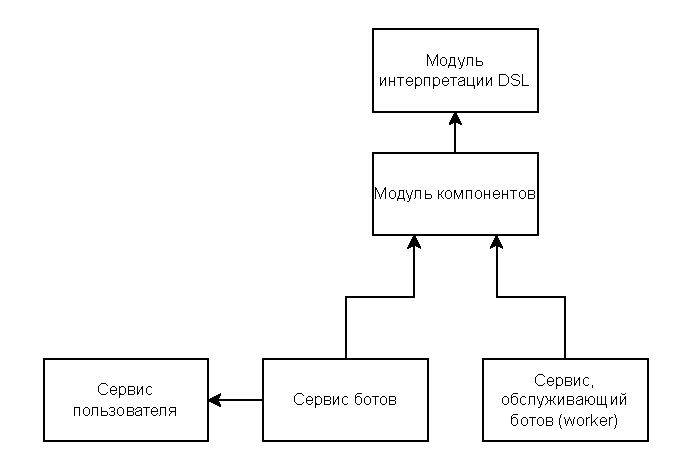
\includegraphics[width=0.7\textwidth]{structures/modules_server_struct.pdf}
	\caption{Модульная структура серверной части конструктора}
	\label{f:modules_server_struct}
\end{figure}

Сервис ботов отвечает за управление состоянием бота и редактирование его компонентной структуры.
Сервис ботов зависит от сервиса пользователей, который предоставляет первому методы для авторизации пользователя.
Также сервис ботов зависит от модуля компонентов, который описывает структуры компонентов и реализует их логику выполнения.

Обслуживающий сервис отвечает за логику работы бота. 
Он выполняет обработку запроса к боту от пользователя Telegram.
В соответствии с разработанной компонентной структурой бота, обслуживающий сервис вызывает методы модуля компонентов для запуска их логики выполнения.

Одним из компонентов является компонент выполнения кода на предметно-ориентированном языке.
Отсюда, модуль компонентов зависит от модуля интерпретации предметно-ориентированного языка.
При запуске компонента выполнения DSL кода, выполняется вызов функции выполнения кода из модуля интерпретации.

Таким образом, в данном проекте для возможности интеграции с серверной частью конструктора Telegram ботов необходимо реализовать программный интерфейс,
который бы предоставлял возможность передачи кода и значений внешних переменных, интерпретатору предметно-ориентированного языка.

Работа интерпретатора состоит из последовательного выполнения следующих этапов:
\begin{enumerate}
	\item лексический анализ;
	\item синтаксический анализ;
	\item семантический анализ;
	\item исполнение команд.
\end{enumerate}

Обобщенная структура интерпретатора представлена на рисунке~\ref{f:full_interpreter_struct}.

\begin{figure}[ht]
	\centering
	\vspace{\toppaddingoffigure}
	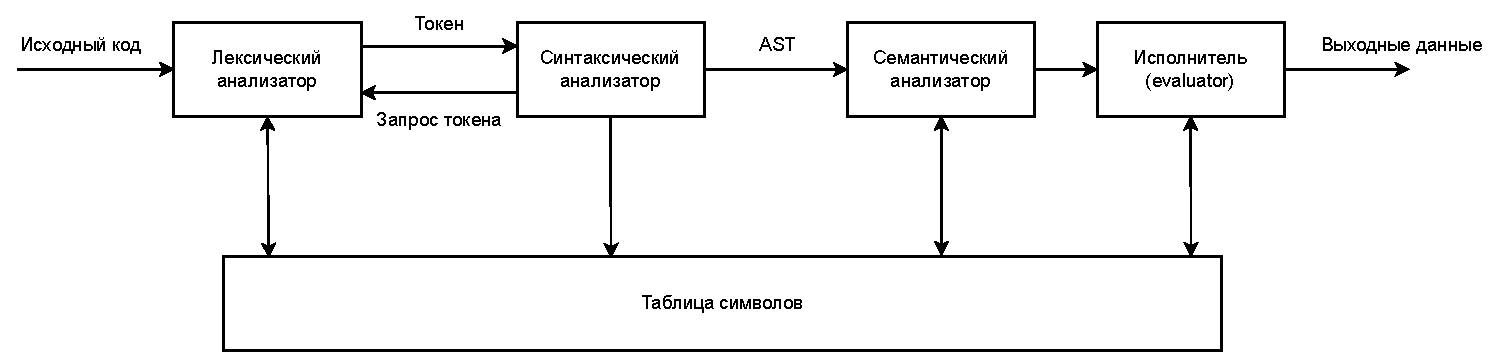
\includegraphics[width=1.0\textwidth]{structures/full_interpreter_struct.pdf}
	\caption{Обобщенная структура интерпретатора}
	\label{f:full_interpreter_struct}
\end{figure}

Для решения поставленной задачи, в первую очередь, необходимо в соответствии с указанными требованиями
разработать грамматику предметно-ориентированного языка и спроектировать обобщенную структуру программы интерпретатора.

\input{pages/content/structures/grammar.tex}
\input{pages/content/structures/lexical_analyzer.tex}
\input{pages/content/structures/parser.tex}
\input{pages/content/structures/semantic_analyzer.tex}
\newpage

\section{Программная реализация}

В данном разделе представлено описание выбранных инструментов разработки для решения поставленной задачи. 
Описана программная реализация модуля интерпретации предметно-ориентированного языка.
Рассмотрены детали реализации его основных структурных частей.
Также выполнено тестирование основных функций программы.

\subsection{Выбор инструментов разработки}

В качестве языка программирования для разработки был выбран Go.

Go (Golang) -- это компилируемый многопоточный язык программирования с открытым исходным кодом, разработанный компанией Google \refref{ref:golang}.

Выбор данного языка обусловлен совместимостью между разрабатываемым модулем и основной системой,
так как для реализации серверной части конструктора Telegram ботов так же был выбран язык Go.
Использование одного языка для всей системы гарантирует,
что модули будут легко интегрироваться друг с другом без необходимости создания сложных интерфейсов или адаптеров.

Язык Go имеет и другие положительные характеристики:
\begin{itemize}
    \item высокая производительность -- Go компилируется в машинный код, что обеспечивает его высокую скорость исполнения;
    \item безопасность типов -- строгая статическая типизация предотвращает множество ошибок на этапе компиляции;
    \item встроенная поддержка параллелизма -- в Go реализованы горутины и каналы -- встроенные механизмы для эффективной работы с параллельными задачами;
    \item расширяемость -- язык имеет встроенную систему управления модулями и широкую экосистему общедоступных библиотек.
\end{itemize}

Выбор языка программирования Go для реализации модуля интерпретации предметно-ориентированного языка конструктора Telegram ботов обоснован тем,
что он позволяет поддерживать единообразие кода, использовать его технические преимущества и соответствовать основным требованиям проекта.

\input{pages/content/implementation/lexer.tex}
\input{pages/content/implementation/parser.tex}
\input{pages/content/implementation/semantic_analyzer.tex}
\input{pages/content/implementation/evaluator.tex}
\input{pages/content/implementation/testing.tex}

\section*{Вывод}

В данном разделе на основании разработанных архитектурно-структурных решениях и алгоритмах функционирования выполнена программная реализация модуля интерпретации предметно-ориентированного языка.
С помощью выбранных инструментов разработки выполнена программная реализация лексического анализатора, синтаксического анализатора, семантического анализатора и исполнителя.

Также на базе встроенной в среду выполнения Go утилиты <<go test>> были реализованы юнит-тесты, охватывающие большинство функций модуля интерпретации.
\newpage

\csection{Заключение}

В ходе выполнения выпускной квалификационной работы выполнена разработка предметно-ориентированного языка для конструктора Telegram ботов и интерпретатора для него.
Основной целью проекта было расширение функциональных возможностей визуального конструктора Telegram ботов.
Благодаря использованию DSL можно более гибко настроить логику работы бота и предоставить пользователю платформы возможность построения сложных, уникальных ботов,
которых было бы невозможно или затруднительно построить с использованием только базового набора компонентов визуального конструктора.

На основе анализа предметной области и определения основных функциональных возможностей предметно-ориентированного языка было сформировано расширенное технического задание,
определяющее требования к разрабатываемому продукту.

Исходя из требований технического задания первоочередной задачей было разработать и описать грамматику предметно-ориентированного языка.
Для описания формальной грамматики была выбрана расширенная форма Бэкуса-Наура.

Была выполнена разработка архитектурно-структурных решений и алгоритмов функционирования каждой составляющей части модуля интерпретации,
а именно лексического, синтаксического, семантического анализаторов и исполнителя инструкций предметно-ориентированного языка.
Также описан программный интерфейс интеграции модуля с серверной частью конструктора.

На этапе программной реализации были выполнено кодирование анализаторов и исполнителя
в соответствии с разработанными алгоритмами функционирования с помощью выбранных инструментов разработки.
Кроме этого было осуществлено модульное тестирование разработанной программы.

Разработанный предметно-ориентированный язык позволяет расширить функциональные возможности конструктора Telegram ботов.
\docappendix{Листинг кода}

\begin{lstlisting}
var a = 1;
var b = 10;
var c = 123;
var d = a + b + c;

some_function(a, b, c);
\end{lstlisting}


\docappendix{Авторская справка}
\input{pages/authornote.example.tex}

\docappendix[справочное]{Какое-то справочное приложение}


Содержимое приложения

% \newpage

\csection{Библиографический список}

\begin{references}
	\item\label{ref:num-methods} Бахвалов Н.С., Жидков Н.П., Кобельников Г.М.
	Численные методы [Текст] – 4-е изд. – М:. БИНОМ. Лаборатория
	знаний, 2006. – 636 с.: ил.
	\item Безрученко Б.П., Смирнов Д.А.
	Статистическое моделирование по временным рядам [Электронный ресурс]
	Cарат. отд-ние Ин-та радиотехники и электроники РАН.
	– Электрон. дан. – Саратов, 2000. – Режим доступа:
	http://www.masters.donntu.edu.ua/2012/fknt/dorosh/library/article4.pdf,
	свободный. - Загл. с экрана.
	\item\label{ref:time-series-analysis} Бокс Дж., Дженкинс Г. Анализ временных рядов.
	Прогноз и управление [Текст]. - М.: Мир, 1974.
\end{references}

} {
	% Пример файла содержимого документа
% Измените подключаемые файлы в зависимости от вашей структуры документа


\csection{Введение}

В современном мире все больше обретают популярность сервисы
визуального конструирования приложений.

Конструктор позволяет широкому кругу пользователей создавать программные продукты с помощью визуального редактора.
Пользователи могут выстраивать логику работы приложения просто перетаскивая визуальные блоки.
Это значительно упрощает разработку и делает её доступной даже для тех, кто не имеет глубоких знаний в программировании.
Однако функциональные возможности такого подхода к построению приложений ограничены и
их зачастую недостаточно для реализации сложных, специфичных программных продуктов.

Расширение возможностей платформы визуального конструктора возможно
за счёт использования предметно-ориентированного языка программирования.
С помощью написания инструкций на данном языке, пользователи  могут гибко задавать логику
работы разрабатываемого приложения.

\pagebreak


\section{Анализ предметной области}

В данном разделе проводится анализ предметной области,
который позволит обосновать актуальность разработки проекта,
приводятся ключевые требования и особенности конструкций,
которые должны быть реализованы в предметно-ориентированном языке визуального конструктора Telegram ботов.

\subsection{Актуальность разработки}

Боты в Telegram являются его популярной особенностью.
С их помощью пользователи могут в интуитивно понятной форме выполнять различные действия, не выходя из мессенджера Telegram.

Боты могут обладать различным функционалом и использоваться в различных сферах, например:
\begin{itemize}
    \item боты для общения с клиентами;
    \item техническая поддержка;
    \item продажа товаров и услуг;
    \item образовательные боты;
    \item боты для знакомств и общения;
    \item развлечения;
    \item утилиты и интрументы.
\end{itemize}

Боты имеют множетство плюсов как для пользователей, так и для их владельцев, например некоторые из них:
\begin{itemize}
    \item замена мобильного приложения;
    \item удобство использования, интерактивное взаимодействие;
    \item интеграция с другими системами;
    \item снижение затрат;
    \item круглосуточный доступ.
\end{itemize}

С ростом популярности ботов на рынке стали появляться визуальные конструкторы Telegram ботов --
решения для разработки и запуска ботов ботов с минимальным написанием программного кода или совсем без него. 

Визуальным конструктором называется NoCode/LowCode инструмент,
предназначенный для быстрого создания приложений без обязательного знания языков программирования общего назначения.
Иными словами, весь процесс разработки -- это взаимодействие с визуальными компонентами платформы,
с помощью которых выстраивается логика работы приложения.
За счет этого конструкторы значительно упрощают и удешевляют разработку и запуск программных продуктов.
Ведь не все обладают знаниями и навыками программирования с использованием языков общего назначения, достаточными для создания даже простых программ.
Кроме того, при наличии конструктора нет необходимости разрабатывать каждый раз отдельное приложение для выполнения типовых задач,
так как конструктор предоставляет необходимый набор инструментов для быстрого создания прототипа \refref{ref:nolowcode}.

Конструкторы имеют некоторые ограничения, например, при их использовании нельзя выйти за рамки возможностей самого конструктора,
а при выходе нового функционала Telegram Bot API,
владельцам платформы визуального конструирования ботов потребуется некоторые время на реализацию поддержки новых методов.

Однако использование только визуальных инструментов накладывает некоторые функциональные ограничения.
Обычно количество предоставляемых конструктором компонентов невелико и каждый из них способен выполнять только некоторую небольшую функцию, например отправить сообщение.
Это значительно ограничивает возможности пользователя в создании уникальных ботов.
Чтобы создание Telegram бота было более гибким, в систему можно интегрировать предметно-ориентированный язык программирования,
направленный на расширение функциональных возможностей визуального конструктора.
В отличие от визуальных блоков – язык позволяет пользователям сервиса гибко описывать логику работы бота.

Предметно-ориентированный язык (domain-specific language, DSL) -- это компьютерный язык, специализированный для конкретной предметной области применения \refref{ref:dsl}.
Противоположностью DSL являются языки общего назначения, такие как C++, Python, Go и т.д.

Примеры предметно-ориентированных языков:
\begin{itemize}
    \item язык запросов SQL -- применяется при работе с базами данных;
    \item shell-скрипты;
    \item HTML -- язык разметки пользовательского веб-интерфейса;
    \item CSS -- каскадные таблицы стилей, описывающие внешний вид веб-страницы.
\end{itemize}

Предметно-ориентированные языка можно разделить на две группы по способу представления конструкций \refref{ref:dsl_classification}:
\begin{enumerate}
    \item текстовые DSL -- текстовая форма, по аналогии с языками общего назначения;
    \item визуальные DSL -- формирование конструкций выполняется в графическом виде.
\end{enumerate}

Визуальные DSL получили большее распространение, поскольку графическое представление информации обладает большей наглядностью.

Также DSL делятся на два типа: внутренние и внешние.

Внутренние языки опираются на язык общего назначения, являются его часть и дополняют его.
Синтаксис такого DSL не может нарушать синтаксис базового языка.

Внешние DSL являются самостоятельными языками, имеют свой синтаксис и семантику.
Для успешного запуска они имеют свой компилятор или интерпретатор.

DSL разрабатываются с учетом особенностей предметной области,
благодаря чему являются менее избыточными по сравнению с языками общего назначения и более понятными для специалистов данной области.
Также предметно-ориентированные языки позволяют работать на более высоком уровне абстракции,
что увеличивает эффективность решения поставленных задач и снижает необходимость в изучении универсальных языков.
DSL языки легче изучать, учитывая их ограниченную область применения.

Помимо приведённых положительных аспектов предметно-ориентированных языков, они имеют некоторые недостатки.
DSL по сравнению с языками общего назначения имеют ограниченные возможности, например, малое разнообразие алгоритмов и структур данных.
Кроме того, разработка и внедрение предметно-ориентированного языка может привести к значительным тратам временных и финансовых ресурсов.

\input{pages/content/techtask.tex}

\section*{Вывод}

В данном разделе был проведен анализ предметной области, в результате чего было определено,
что визуальные конструкторы значительно упрощают процесс создания и запуска Telegram ботов,
однако, они имеет функциональные ограничения, которые препятствуют разработке продукта со сложной логикой работы.
Предметно-ориентированный язык позволяет расширить возможности визуального конструктора и создавать уникальных ботов,
в соответствии с пользовательскими потребностями.

Также было рассмотрено расширенное техническое задание,
в котором были определены цели и задачи разработки и основные требования к разрабатываемому программному продукту.

Основываясь на этом можно приступить к разработке предметно-ориентированного языка для визуального конструктора Telegram ботов,
так как рассмотренная проблема является актуальной.
\newpage

\section{Разработка архитектурно-структурных решений}

Выполнение кода предметно-ориентированного языка осуществляется за счет интерпретатора,
который должен быть спроектирован в виде модуля, подключаемого к серверной части конструктора Telegram ботов.

Обобщенная модульная структура серверной части конструктора представлена на рисунке~\ref{f:modules_server_struct}.

\begin{figure}[ht]
	\centering
	\vspace{\toppaddingoffigure}
	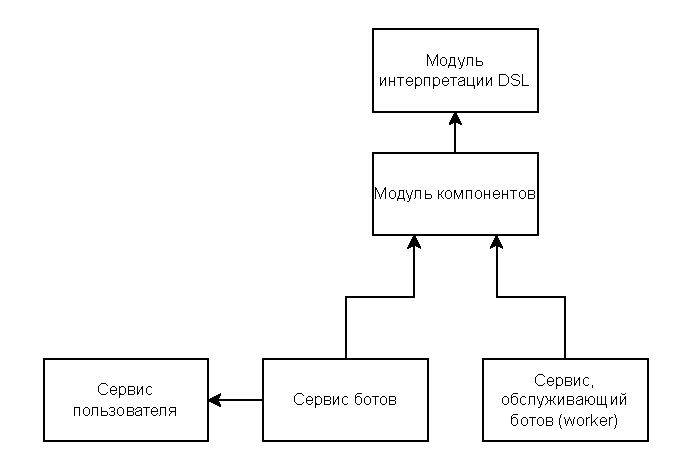
\includegraphics[width=0.7\textwidth]{structures/modules_server_struct.pdf}
	\caption{Модульная структура серверной части конструктора}
	\label{f:modules_server_struct}
\end{figure}

Сервис ботов отвечает за управление состоянием бота и редактирование его компонентной структуры.
Сервис ботов зависит от сервиса пользователей, который предоставляет первому методы для авторизации пользователя.
Также сервис ботов зависит от модуля компонентов, который описывает структуры компонентов и реализует их логику выполнения.

Обслуживающий сервис отвечает за логику работы бота. 
Он выполняет обработку запроса к боту от пользователя Telegram.
В соответствии с разработанной компонентной структурой бота, обслуживающий сервис вызывает методы модуля компонентов для запуска их логики выполнения.

Одним из компонентов является компонент выполнения кода на предметно-ориентированном языке.
Отсюда, модуль компонентов зависит от модуля интерпретации предметно-ориентированного языка.
При запуске компонента выполнения DSL кода, выполняется вызов функции выполнения кода из модуля интерпретации.

Таким образом, в данном проекте для возможности интеграции с серверной частью конструктора Telegram ботов необходимо реализовать программный интерфейс,
который бы предоставлял возможность передачи кода и значений внешних переменных, интерпретатору предметно-ориентированного языка.

Работа интерпретатора состоит из последовательного выполнения следующих этапов:
\begin{enumerate}
	\item лексический анализ;
	\item синтаксический анализ;
	\item семантический анализ;
	\item исполнение команд.
\end{enumerate}

Обобщенная структура интерпретатора представлена на рисунке~\ref{f:full_interpreter_struct}.

\begin{figure}[ht]
	\centering
	\vspace{\toppaddingoffigure}
	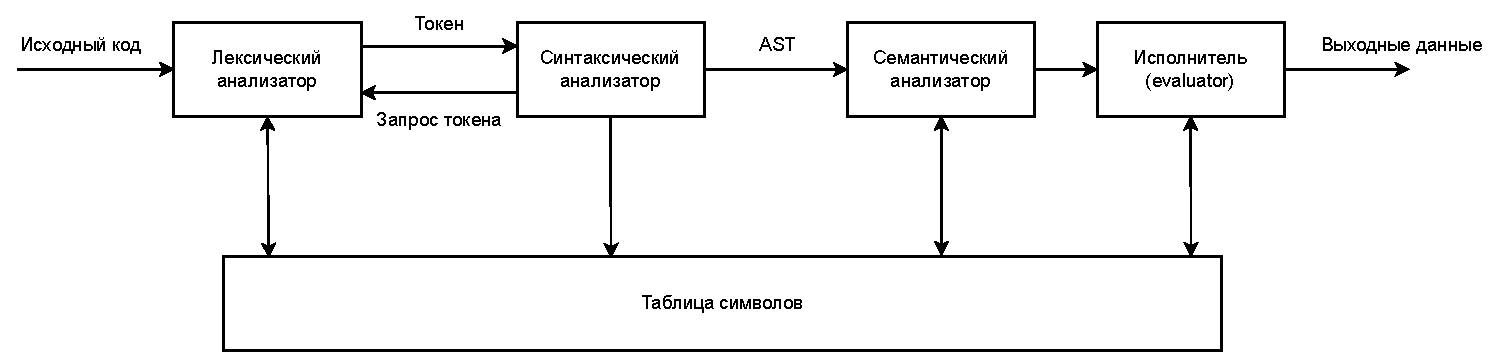
\includegraphics[width=1.0\textwidth]{structures/full_interpreter_struct.pdf}
	\caption{Обобщенная структура интерпретатора}
	\label{f:full_interpreter_struct}
\end{figure}

Для решения поставленной задачи, в первую очередь, необходимо в соответствии с указанными требованиями
разработать грамматику предметно-ориентированного языка и спроектировать обобщенную структуру программы интерпретатора.

\input{pages/content/structures/grammar.tex}
\input{pages/content/structures/lexical_analyzer.tex}
\input{pages/content/structures/parser.tex}
\input{pages/content/structures/semantic_analyzer.tex}
\newpage

\section{Программная реализация}

В данном разделе представлено описание выбранных инструментов разработки для решения поставленной задачи. 
Описана программная реализация модуля интерпретации предметно-ориентированного языка.
Рассмотрены детали реализации его основных структурных частей.
Также выполнено тестирование основных функций программы.

\subsection{Выбор инструментов разработки}

В качестве языка программирования для разработки был выбран Go.

Go (Golang) -- это компилируемый многопоточный язык программирования с открытым исходным кодом, разработанный компанией Google \refref{ref:golang}.

Выбор данного языка обусловлен совместимостью между разрабатываемым модулем и основной системой,
так как для реализации серверной части конструктора Telegram ботов так же был выбран язык Go.
Использование одного языка для всей системы гарантирует,
что модули будут легко интегрироваться друг с другом без необходимости создания сложных интерфейсов или адаптеров.

Язык Go имеет и другие положительные характеристики:
\begin{itemize}
    \item высокая производительность -- Go компилируется в машинный код, что обеспечивает его высокую скорость исполнения;
    \item безопасность типов -- строгая статическая типизация предотвращает множество ошибок на этапе компиляции;
    \item встроенная поддержка параллелизма -- в Go реализованы горутины и каналы -- встроенные механизмы для эффективной работы с параллельными задачами;
    \item расширяемость -- язык имеет встроенную систему управления модулями и широкую экосистему общедоступных библиотек.
\end{itemize}

Выбор языка программирования Go для реализации модуля интерпретации предметно-ориентированного языка конструктора Telegram ботов обоснован тем,
что он позволяет поддерживать единообразие кода, использовать его технические преимущества и соответствовать основным требованиям проекта.

\input{pages/content/implementation/lexer.tex}
\input{pages/content/implementation/parser.tex}
\input{pages/content/implementation/semantic_analyzer.tex}
\input{pages/content/implementation/evaluator.tex}
\input{pages/content/implementation/testing.tex}

\section*{Вывод}

В данном разделе на основании разработанных архитектурно-структурных решениях и алгоритмах функционирования выполнена программная реализация модуля интерпретации предметно-ориентированного языка.
С помощью выбранных инструментов разработки выполнена программная реализация лексического анализатора, синтаксического анализатора, семантического анализатора и исполнителя.

Также на базе встроенной в среду выполнения Go утилиты <<go test>> были реализованы юнит-тесты, охватывающие большинство функций модуля интерпретации.
\newpage

\csection{Заключение}

В ходе выполнения выпускной квалификационной работы выполнена разработка предметно-ориентированного языка для конструктора Telegram ботов и интерпретатора для него.
Основной целью проекта было расширение функциональных возможностей визуального конструктора Telegram ботов.
Благодаря использованию DSL можно более гибко настроить логику работы бота и предоставить пользователю платформы возможность построения сложных, уникальных ботов,
которых было бы невозможно или затруднительно построить с использованием только базового набора компонентов визуального конструктора.

На основе анализа предметной области и определения основных функциональных возможностей предметно-ориентированного языка было сформировано расширенное технического задание,
определяющее требования к разрабатываемому продукту.

Исходя из требований технического задания первоочередной задачей было разработать и описать грамматику предметно-ориентированного языка.
Для описания формальной грамматики была выбрана расширенная форма Бэкуса-Наура.

Была выполнена разработка архитектурно-структурных решений и алгоритмов функционирования каждой составляющей части модуля интерпретации,
а именно лексического, синтаксического, семантического анализаторов и исполнителя инструкций предметно-ориентированного языка.
Также описан программный интерфейс интеграции модуля с серверной частью конструктора.

На этапе программной реализации были выполнено кодирование анализаторов и исполнителя
в соответствии с разработанными алгоритмами функционирования с помощью выбранных инструментов разработки.
Кроме этого было осуществлено модульное тестирование разработанной программы.

Разработанный предметно-ориентированный язык позволяет расширить функциональные возможности конструктора Telegram ботов.
\docappendix{Листинг кода}

\begin{lstlisting}
var a = 1;
var b = 10;
var c = 123;
var d = a + b + c;

some_function(a, b, c);
\end{lstlisting}


\docappendix{Авторская справка}
\input{pages/authornote.example.tex}

\docappendix[справочное]{Какое-то справочное приложение}


Содержимое приложения

% \newpage

\csection{Библиографический список}

\begin{references}
	\item\label{ref:num-methods} Бахвалов Н.С., Жидков Н.П., Кобельников Г.М.
	Численные методы [Текст] – 4-е изд. – М:. БИНОМ. Лаборатория
	знаний, 2006. – 636 с.: ил.
	\item Безрученко Б.П., Смирнов Д.А.
	Статистическое моделирование по временным рядам [Электронный ресурс]
	Cарат. отд-ние Ин-та радиотехники и электроники РАН.
	– Электрон. дан. – Саратов, 2000. – Режим доступа:
	http://www.masters.donntu.edu.ua/2012/fknt/dorosh/library/article4.pdf,
	свободный. - Загл. с экрана.
	\item\label{ref:time-series-analysis} Бокс Дж., Дженкинс Г. Анализ временных рядов.
	Прогноз и управление [Текст]. - М.: Мир, 1974.
\end{references}

}

}

}{
	
{

\vspace{0.8cm}
\begin{center}
	Реферат
\end{center}

\vspace{1em}

\authorwithinitials\
\topic
:\
\mbox{\tpga}\
ВКР / ВятГУ, каф. ЭВМ; рук.
\supervisor – Киров, \the\year. –
Гр.ч. \numberofposters л. ф.А1;
ПЗ
\total{page} с.,
\total{figure} рис.,
\total{table} табл.,
\total{equation} форм.,
\ref*{ref:total} источников,
\total{appendix} прил.

\vspace{1.5em}

\IfFileExists{pages/abstract/tags.tex}{
	КОНСТРУКТОР,
ПРЕДМЕТНО-ОРИЕНТИРОВАННЫЙ ЯЗЫК,
ГРАММАТИКА,
ЛЕКСИЧЕСКИЙ АНАЛИЗ,
СИНТАКСИЧЕСКИЙ АНАЛИЗ,
СЕМАНТИЧЕСКИЙ АНАЛИЗ,
ИНТЕРПРЕТАЦИЯ,
Go.

}{
	КОНСТРУКТОР,
ПРЕДМЕТНО-ОРИЕНТИРОВАННЫЙ ЯЗЫК,
ГРАММАТИКА,
ЛЕКСИЧЕСКИЙ АНАЛИЗ,
СИНТАКСИЧЕСКИЙ АНАЛИЗ,
СЕМАНТИЧЕСКИЙ АНАЛИЗ,
ИНТЕРПРЕТАЦИЯ,
Go.

}

\vspace{1.5em}

\IfFileExists{pages/abstract/content.tex}{
	% Пример файла содержимого документа
% Измените подключаемые файлы в зависимости от вашей структуры документа


\csection{Введение}

В современном мире все больше обретают популярность сервисы
визуального конструирования приложений.

Конструктор позволяет широкому кругу пользователей создавать программные продукты с помощью визуального редактора.
Пользователи могут выстраивать логику работы приложения просто перетаскивая визуальные блоки.
Это значительно упрощает разработку и делает её доступной даже для тех, кто не имеет глубоких знаний в программировании.
Однако функциональные возможности такого подхода к построению приложений ограничены и
их зачастую недостаточно для реализации сложных, специфичных программных продуктов.

Расширение возможностей платформы визуального конструктора возможно
за счёт использования предметно-ориентированного языка программирования.
С помощью написания инструкций на данном языке, пользователи  могут гибко задавать логику
работы разрабатываемого приложения.

\pagebreak


\section{Анализ предметной области}

В данном разделе проводится анализ предметной области,
который позволит обосновать актуальность разработки проекта,
приводятся ключевые требования и особенности конструкций,
которые должны быть реализованы в предметно-ориентированном языке визуального конструктора Telegram ботов.

\subsection{Актуальность разработки}

Боты в Telegram являются его популярной особенностью.
С их помощью пользователи могут в интуитивно понятной форме выполнять различные действия, не выходя из мессенджера Telegram.

Боты могут обладать различным функционалом и использоваться в различных сферах, например:
\begin{itemize}
    \item боты для общения с клиентами;
    \item техническая поддержка;
    \item продажа товаров и услуг;
    \item образовательные боты;
    \item боты для знакомств и общения;
    \item развлечения;
    \item утилиты и интрументы.
\end{itemize}

Боты имеют множетство плюсов как для пользователей, так и для их владельцев, например некоторые из них:
\begin{itemize}
    \item замена мобильного приложения;
    \item удобство использования, интерактивное взаимодействие;
    \item интеграция с другими системами;
    \item снижение затрат;
    \item круглосуточный доступ.
\end{itemize}

С ростом популярности ботов на рынке стали появляться визуальные конструкторы Telegram ботов --
решения для разработки и запуска ботов ботов с минимальным написанием программного кода или совсем без него. 

Визуальным конструктором называется NoCode/LowCode инструмент,
предназначенный для быстрого создания приложений без обязательного знания языков программирования общего назначения.
Иными словами, весь процесс разработки -- это взаимодействие с визуальными компонентами платформы,
с помощью которых выстраивается логика работы приложения.
За счет этого конструкторы значительно упрощают и удешевляют разработку и запуск программных продуктов.
Ведь не все обладают знаниями и навыками программирования с использованием языков общего назначения, достаточными для создания даже простых программ.
Кроме того, при наличии конструктора нет необходимости разрабатывать каждый раз отдельное приложение для выполнения типовых задач,
так как конструктор предоставляет необходимый набор инструментов для быстрого создания прототипа \refref{ref:nolowcode}.

Конструкторы имеют некоторые ограничения, например, при их использовании нельзя выйти за рамки возможностей самого конструктора,
а при выходе нового функционала Telegram Bot API,
владельцам платформы визуального конструирования ботов потребуется некоторые время на реализацию поддержки новых методов.

Однако использование только визуальных инструментов накладывает некоторые функциональные ограничения.
Обычно количество предоставляемых конструктором компонентов невелико и каждый из них способен выполнять только некоторую небольшую функцию, например отправить сообщение.
Это значительно ограничивает возможности пользователя в создании уникальных ботов.
Чтобы создание Telegram бота было более гибким, в систему можно интегрировать предметно-ориентированный язык программирования,
направленный на расширение функциональных возможностей визуального конструктора.
В отличие от визуальных блоков – язык позволяет пользователям сервиса гибко описывать логику работы бота.

Предметно-ориентированный язык (domain-specific language, DSL) -- это компьютерный язык, специализированный для конкретной предметной области применения \refref{ref:dsl}.
Противоположностью DSL являются языки общего назначения, такие как C++, Python, Go и т.д.

Примеры предметно-ориентированных языков:
\begin{itemize}
    \item язык запросов SQL -- применяется при работе с базами данных;
    \item shell-скрипты;
    \item HTML -- язык разметки пользовательского веб-интерфейса;
    \item CSS -- каскадные таблицы стилей, описывающие внешний вид веб-страницы.
\end{itemize}

Предметно-ориентированные языка можно разделить на две группы по способу представления конструкций \refref{ref:dsl_classification}:
\begin{enumerate}
    \item текстовые DSL -- текстовая форма, по аналогии с языками общего назначения;
    \item визуальные DSL -- формирование конструкций выполняется в графическом виде.
\end{enumerate}

Визуальные DSL получили большее распространение, поскольку графическое представление информации обладает большей наглядностью.

Также DSL делятся на два типа: внутренние и внешние.

Внутренние языки опираются на язык общего назначения, являются его часть и дополняют его.
Синтаксис такого DSL не может нарушать синтаксис базового языка.

Внешние DSL являются самостоятельными языками, имеют свой синтаксис и семантику.
Для успешного запуска они имеют свой компилятор или интерпретатор.

DSL разрабатываются с учетом особенностей предметной области,
благодаря чему являются менее избыточными по сравнению с языками общего назначения и более понятными для специалистов данной области.
Также предметно-ориентированные языки позволяют работать на более высоком уровне абстракции,
что увеличивает эффективность решения поставленных задач и снижает необходимость в изучении универсальных языков.
DSL языки легче изучать, учитывая их ограниченную область применения.

Помимо приведённых положительных аспектов предметно-ориентированных языков, они имеют некоторые недостатки.
DSL по сравнению с языками общего назначения имеют ограниченные возможности, например, малое разнообразие алгоритмов и структур данных.
Кроме того, разработка и внедрение предметно-ориентированного языка может привести к значительным тратам временных и финансовых ресурсов.

\input{pages/content/techtask.tex}

\section*{Вывод}

В данном разделе был проведен анализ предметной области, в результате чего было определено,
что визуальные конструкторы значительно упрощают процесс создания и запуска Telegram ботов,
однако, они имеет функциональные ограничения, которые препятствуют разработке продукта со сложной логикой работы.
Предметно-ориентированный язык позволяет расширить возможности визуального конструктора и создавать уникальных ботов,
в соответствии с пользовательскими потребностями.

Также было рассмотрено расширенное техническое задание,
в котором были определены цели и задачи разработки и основные требования к разрабатываемому программному продукту.

Основываясь на этом можно приступить к разработке предметно-ориентированного языка для визуального конструктора Telegram ботов,
так как рассмотренная проблема является актуальной.
\newpage

\section{Разработка архитектурно-структурных решений}

Выполнение кода предметно-ориентированного языка осуществляется за счет интерпретатора,
который должен быть спроектирован в виде модуля, подключаемого к серверной части конструктора Telegram ботов.

Обобщенная модульная структура серверной части конструктора представлена на рисунке~\ref{f:modules_server_struct}.

\begin{figure}[ht]
	\centering
	\vspace{\toppaddingoffigure}
	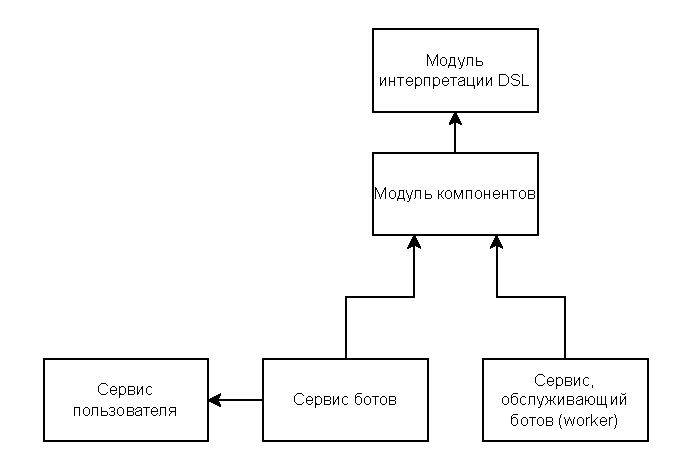
\includegraphics[width=0.7\textwidth]{structures/modules_server_struct.pdf}
	\caption{Модульная структура серверной части конструктора}
	\label{f:modules_server_struct}
\end{figure}

Сервис ботов отвечает за управление состоянием бота и редактирование его компонентной структуры.
Сервис ботов зависит от сервиса пользователей, который предоставляет первому методы для авторизации пользователя.
Также сервис ботов зависит от модуля компонентов, который описывает структуры компонентов и реализует их логику выполнения.

Обслуживающий сервис отвечает за логику работы бота. 
Он выполняет обработку запроса к боту от пользователя Telegram.
В соответствии с разработанной компонентной структурой бота, обслуживающий сервис вызывает методы модуля компонентов для запуска их логики выполнения.

Одним из компонентов является компонент выполнения кода на предметно-ориентированном языке.
Отсюда, модуль компонентов зависит от модуля интерпретации предметно-ориентированного языка.
При запуске компонента выполнения DSL кода, выполняется вызов функции выполнения кода из модуля интерпретации.

Таким образом, в данном проекте для возможности интеграции с серверной частью конструктора Telegram ботов необходимо реализовать программный интерфейс,
который бы предоставлял возможность передачи кода и значений внешних переменных, интерпретатору предметно-ориентированного языка.

Работа интерпретатора состоит из последовательного выполнения следующих этапов:
\begin{enumerate}
	\item лексический анализ;
	\item синтаксический анализ;
	\item семантический анализ;
	\item исполнение команд.
\end{enumerate}

Обобщенная структура интерпретатора представлена на рисунке~\ref{f:full_interpreter_struct}.

\begin{figure}[ht]
	\centering
	\vspace{\toppaddingoffigure}
	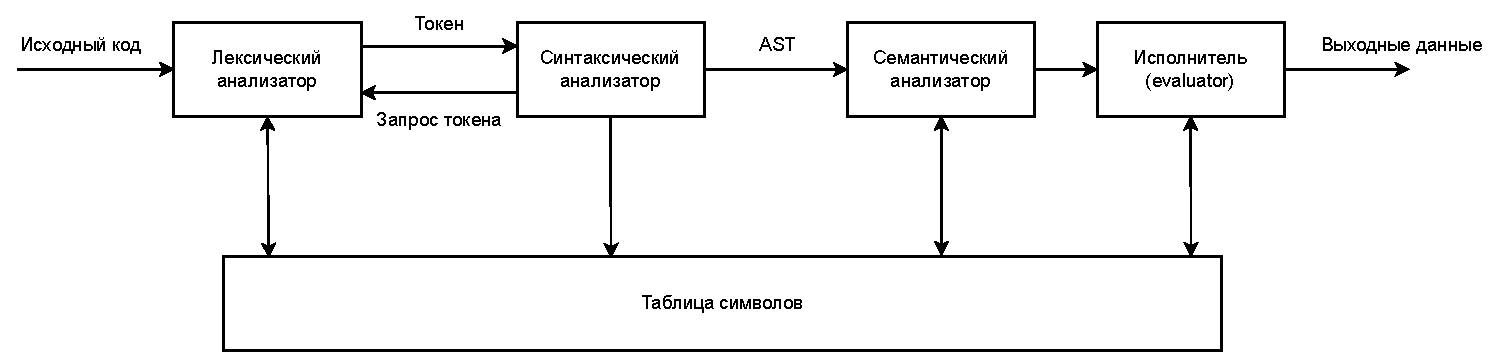
\includegraphics[width=1.0\textwidth]{structures/full_interpreter_struct.pdf}
	\caption{Обобщенная структура интерпретатора}
	\label{f:full_interpreter_struct}
\end{figure}

Для решения поставленной задачи, в первую очередь, необходимо в соответствии с указанными требованиями
разработать грамматику предметно-ориентированного языка и спроектировать обобщенную структуру программы интерпретатора.

\input{pages/content/structures/grammar.tex}
\input{pages/content/structures/lexical_analyzer.tex}
\input{pages/content/structures/parser.tex}
\input{pages/content/structures/semantic_analyzer.tex}
\newpage

\section{Программная реализация}

В данном разделе представлено описание выбранных инструментов разработки для решения поставленной задачи. 
Описана программная реализация модуля интерпретации предметно-ориентированного языка.
Рассмотрены детали реализации его основных структурных частей.
Также выполнено тестирование основных функций программы.

\subsection{Выбор инструментов разработки}

В качестве языка программирования для разработки был выбран Go.

Go (Golang) -- это компилируемый многопоточный язык программирования с открытым исходным кодом, разработанный компанией Google \refref{ref:golang}.

Выбор данного языка обусловлен совместимостью между разрабатываемым модулем и основной системой,
так как для реализации серверной части конструктора Telegram ботов так же был выбран язык Go.
Использование одного языка для всей системы гарантирует,
что модули будут легко интегрироваться друг с другом без необходимости создания сложных интерфейсов или адаптеров.

Язык Go имеет и другие положительные характеристики:
\begin{itemize}
    \item высокая производительность -- Go компилируется в машинный код, что обеспечивает его высокую скорость исполнения;
    \item безопасность типов -- строгая статическая типизация предотвращает множество ошибок на этапе компиляции;
    \item встроенная поддержка параллелизма -- в Go реализованы горутины и каналы -- встроенные механизмы для эффективной работы с параллельными задачами;
    \item расширяемость -- язык имеет встроенную систему управления модулями и широкую экосистему общедоступных библиотек.
\end{itemize}

Выбор языка программирования Go для реализации модуля интерпретации предметно-ориентированного языка конструктора Telegram ботов обоснован тем,
что он позволяет поддерживать единообразие кода, использовать его технические преимущества и соответствовать основным требованиям проекта.

\input{pages/content/implementation/lexer.tex}
\input{pages/content/implementation/parser.tex}
\input{pages/content/implementation/semantic_analyzer.tex}
\input{pages/content/implementation/evaluator.tex}
\input{pages/content/implementation/testing.tex}

\section*{Вывод}

В данном разделе на основании разработанных архитектурно-структурных решениях и алгоритмах функционирования выполнена программная реализация модуля интерпретации предметно-ориентированного языка.
С помощью выбранных инструментов разработки выполнена программная реализация лексического анализатора, синтаксического анализатора, семантического анализатора и исполнителя.

Также на базе встроенной в среду выполнения Go утилиты <<go test>> были реализованы юнит-тесты, охватывающие большинство функций модуля интерпретации.
\newpage

\csection{Заключение}

В ходе выполнения выпускной квалификационной работы выполнена разработка предметно-ориентированного языка для конструктора Telegram ботов и интерпретатора для него.
Основной целью проекта было расширение функциональных возможностей визуального конструктора Telegram ботов.
Благодаря использованию DSL можно более гибко настроить логику работы бота и предоставить пользователю платформы возможность построения сложных, уникальных ботов,
которых было бы невозможно или затруднительно построить с использованием только базового набора компонентов визуального конструктора.

На основе анализа предметной области и определения основных функциональных возможностей предметно-ориентированного языка было сформировано расширенное технического задание,
определяющее требования к разрабатываемому продукту.

Исходя из требований технического задания первоочередной задачей было разработать и описать грамматику предметно-ориентированного языка.
Для описания формальной грамматики была выбрана расширенная форма Бэкуса-Наура.

Была выполнена разработка архитектурно-структурных решений и алгоритмов функционирования каждой составляющей части модуля интерпретации,
а именно лексического, синтаксического, семантического анализаторов и исполнителя инструкций предметно-ориентированного языка.
Также описан программный интерфейс интеграции модуля с серверной частью конструктора.

На этапе программной реализации были выполнено кодирование анализаторов и исполнителя
в соответствии с разработанными алгоритмами функционирования с помощью выбранных инструментов разработки.
Кроме этого было осуществлено модульное тестирование разработанной программы.

Разработанный предметно-ориентированный язык позволяет расширить функциональные возможности конструктора Telegram ботов.
\docappendix{Листинг кода}

\begin{lstlisting}
var a = 1;
var b = 10;
var c = 123;
var d = a + b + c;

some_function(a, b, c);
\end{lstlisting}


\docappendix{Авторская справка}
\input{pages/authornote.example.tex}

\docappendix[справочное]{Какое-то справочное приложение}


Содержимое приложения

% \newpage

\csection{Библиографический список}

\begin{references}
	\item\label{ref:num-methods} Бахвалов Н.С., Жидков Н.П., Кобельников Г.М.
	Численные методы [Текст] – 4-е изд. – М:. БИНОМ. Лаборатория
	знаний, 2006. – 636 с.: ил.
	\item Безрученко Б.П., Смирнов Д.А.
	Статистическое моделирование по временным рядам [Электронный ресурс]
	Cарат. отд-ние Ин-та радиотехники и электроники РАН.
	– Электрон. дан. – Саратов, 2000. – Режим доступа:
	http://www.masters.donntu.edu.ua/2012/fknt/dorosh/library/article4.pdf,
	свободный. - Загл. с экрана.
	\item\label{ref:time-series-analysis} Бокс Дж., Дженкинс Г. Анализ временных рядов.
	Прогноз и управление [Текст]. - М.: Мир, 1974.
\end{references}

} {
	% Пример файла содержимого документа
% Измените подключаемые файлы в зависимости от вашей структуры документа


\csection{Введение}

В современном мире все больше обретают популярность сервисы
визуального конструирования приложений.

Конструктор позволяет широкому кругу пользователей создавать программные продукты с помощью визуального редактора.
Пользователи могут выстраивать логику работы приложения просто перетаскивая визуальные блоки.
Это значительно упрощает разработку и делает её доступной даже для тех, кто не имеет глубоких знаний в программировании.
Однако функциональные возможности такого подхода к построению приложений ограничены и
их зачастую недостаточно для реализации сложных, специфичных программных продуктов.

Расширение возможностей платформы визуального конструктора возможно
за счёт использования предметно-ориентированного языка программирования.
С помощью написания инструкций на данном языке, пользователи  могут гибко задавать логику
работы разрабатываемого приложения.

\pagebreak


\section{Анализ предметной области}

В данном разделе проводится анализ предметной области,
который позволит обосновать актуальность разработки проекта,
приводятся ключевые требования и особенности конструкций,
которые должны быть реализованы в предметно-ориентированном языке визуального конструктора Telegram ботов.

\subsection{Актуальность разработки}

Боты в Telegram являются его популярной особенностью.
С их помощью пользователи могут в интуитивно понятной форме выполнять различные действия, не выходя из мессенджера Telegram.

Боты могут обладать различным функционалом и использоваться в различных сферах, например:
\begin{itemize}
    \item боты для общения с клиентами;
    \item техническая поддержка;
    \item продажа товаров и услуг;
    \item образовательные боты;
    \item боты для знакомств и общения;
    \item развлечения;
    \item утилиты и интрументы.
\end{itemize}

Боты имеют множетство плюсов как для пользователей, так и для их владельцев, например некоторые из них:
\begin{itemize}
    \item замена мобильного приложения;
    \item удобство использования, интерактивное взаимодействие;
    \item интеграция с другими системами;
    \item снижение затрат;
    \item круглосуточный доступ.
\end{itemize}

С ростом популярности ботов на рынке стали появляться визуальные конструкторы Telegram ботов --
решения для разработки и запуска ботов ботов с минимальным написанием программного кода или совсем без него. 

Визуальным конструктором называется NoCode/LowCode инструмент,
предназначенный для быстрого создания приложений без обязательного знания языков программирования общего назначения.
Иными словами, весь процесс разработки -- это взаимодействие с визуальными компонентами платформы,
с помощью которых выстраивается логика работы приложения.
За счет этого конструкторы значительно упрощают и удешевляют разработку и запуск программных продуктов.
Ведь не все обладают знаниями и навыками программирования с использованием языков общего назначения, достаточными для создания даже простых программ.
Кроме того, при наличии конструктора нет необходимости разрабатывать каждый раз отдельное приложение для выполнения типовых задач,
так как конструктор предоставляет необходимый набор инструментов для быстрого создания прототипа \refref{ref:nolowcode}.

Конструкторы имеют некоторые ограничения, например, при их использовании нельзя выйти за рамки возможностей самого конструктора,
а при выходе нового функционала Telegram Bot API,
владельцам платформы визуального конструирования ботов потребуется некоторые время на реализацию поддержки новых методов.

Однако использование только визуальных инструментов накладывает некоторые функциональные ограничения.
Обычно количество предоставляемых конструктором компонентов невелико и каждый из них способен выполнять только некоторую небольшую функцию, например отправить сообщение.
Это значительно ограничивает возможности пользователя в создании уникальных ботов.
Чтобы создание Telegram бота было более гибким, в систему можно интегрировать предметно-ориентированный язык программирования,
направленный на расширение функциональных возможностей визуального конструктора.
В отличие от визуальных блоков – язык позволяет пользователям сервиса гибко описывать логику работы бота.

Предметно-ориентированный язык (domain-specific language, DSL) -- это компьютерный язык, специализированный для конкретной предметной области применения \refref{ref:dsl}.
Противоположностью DSL являются языки общего назначения, такие как C++, Python, Go и т.д.

Примеры предметно-ориентированных языков:
\begin{itemize}
    \item язык запросов SQL -- применяется при работе с базами данных;
    \item shell-скрипты;
    \item HTML -- язык разметки пользовательского веб-интерфейса;
    \item CSS -- каскадные таблицы стилей, описывающие внешний вид веб-страницы.
\end{itemize}

Предметно-ориентированные языка можно разделить на две группы по способу представления конструкций \refref{ref:dsl_classification}:
\begin{enumerate}
    \item текстовые DSL -- текстовая форма, по аналогии с языками общего назначения;
    \item визуальные DSL -- формирование конструкций выполняется в графическом виде.
\end{enumerate}

Визуальные DSL получили большее распространение, поскольку графическое представление информации обладает большей наглядностью.

Также DSL делятся на два типа: внутренние и внешние.

Внутренние языки опираются на язык общего назначения, являются его часть и дополняют его.
Синтаксис такого DSL не может нарушать синтаксис базового языка.

Внешние DSL являются самостоятельными языками, имеют свой синтаксис и семантику.
Для успешного запуска они имеют свой компилятор или интерпретатор.

DSL разрабатываются с учетом особенностей предметной области,
благодаря чему являются менее избыточными по сравнению с языками общего назначения и более понятными для специалистов данной области.
Также предметно-ориентированные языки позволяют работать на более высоком уровне абстракции,
что увеличивает эффективность решения поставленных задач и снижает необходимость в изучении универсальных языков.
DSL языки легче изучать, учитывая их ограниченную область применения.

Помимо приведённых положительных аспектов предметно-ориентированных языков, они имеют некоторые недостатки.
DSL по сравнению с языками общего назначения имеют ограниченные возможности, например, малое разнообразие алгоритмов и структур данных.
Кроме того, разработка и внедрение предметно-ориентированного языка может привести к значительным тратам временных и финансовых ресурсов.

\input{pages/content/techtask.tex}

\section*{Вывод}

В данном разделе был проведен анализ предметной области, в результате чего было определено,
что визуальные конструкторы значительно упрощают процесс создания и запуска Telegram ботов,
однако, они имеет функциональные ограничения, которые препятствуют разработке продукта со сложной логикой работы.
Предметно-ориентированный язык позволяет расширить возможности визуального конструктора и создавать уникальных ботов,
в соответствии с пользовательскими потребностями.

Также было рассмотрено расширенное техническое задание,
в котором были определены цели и задачи разработки и основные требования к разрабатываемому программному продукту.

Основываясь на этом можно приступить к разработке предметно-ориентированного языка для визуального конструктора Telegram ботов,
так как рассмотренная проблема является актуальной.
\newpage

\section{Разработка архитектурно-структурных решений}

Выполнение кода предметно-ориентированного языка осуществляется за счет интерпретатора,
который должен быть спроектирован в виде модуля, подключаемого к серверной части конструктора Telegram ботов.

Обобщенная модульная структура серверной части конструктора представлена на рисунке~\ref{f:modules_server_struct}.

\begin{figure}[ht]
	\centering
	\vspace{\toppaddingoffigure}
	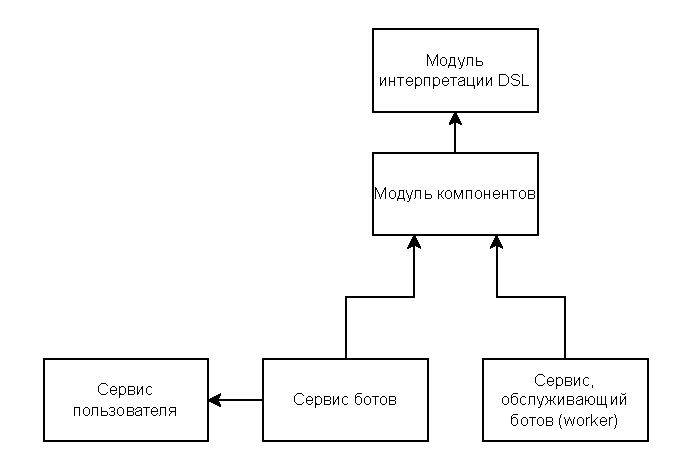
\includegraphics[width=0.7\textwidth]{structures/modules_server_struct.pdf}
	\caption{Модульная структура серверной части конструктора}
	\label{f:modules_server_struct}
\end{figure}

Сервис ботов отвечает за управление состоянием бота и редактирование его компонентной структуры.
Сервис ботов зависит от сервиса пользователей, который предоставляет первому методы для авторизации пользователя.
Также сервис ботов зависит от модуля компонентов, который описывает структуры компонентов и реализует их логику выполнения.

Обслуживающий сервис отвечает за логику работы бота. 
Он выполняет обработку запроса к боту от пользователя Telegram.
В соответствии с разработанной компонентной структурой бота, обслуживающий сервис вызывает методы модуля компонентов для запуска их логики выполнения.

Одним из компонентов является компонент выполнения кода на предметно-ориентированном языке.
Отсюда, модуль компонентов зависит от модуля интерпретации предметно-ориентированного языка.
При запуске компонента выполнения DSL кода, выполняется вызов функции выполнения кода из модуля интерпретации.

Таким образом, в данном проекте для возможности интеграции с серверной частью конструктора Telegram ботов необходимо реализовать программный интерфейс,
который бы предоставлял возможность передачи кода и значений внешних переменных, интерпретатору предметно-ориентированного языка.

Работа интерпретатора состоит из последовательного выполнения следующих этапов:
\begin{enumerate}
	\item лексический анализ;
	\item синтаксический анализ;
	\item семантический анализ;
	\item исполнение команд.
\end{enumerate}

Обобщенная структура интерпретатора представлена на рисунке~\ref{f:full_interpreter_struct}.

\begin{figure}[ht]
	\centering
	\vspace{\toppaddingoffigure}
	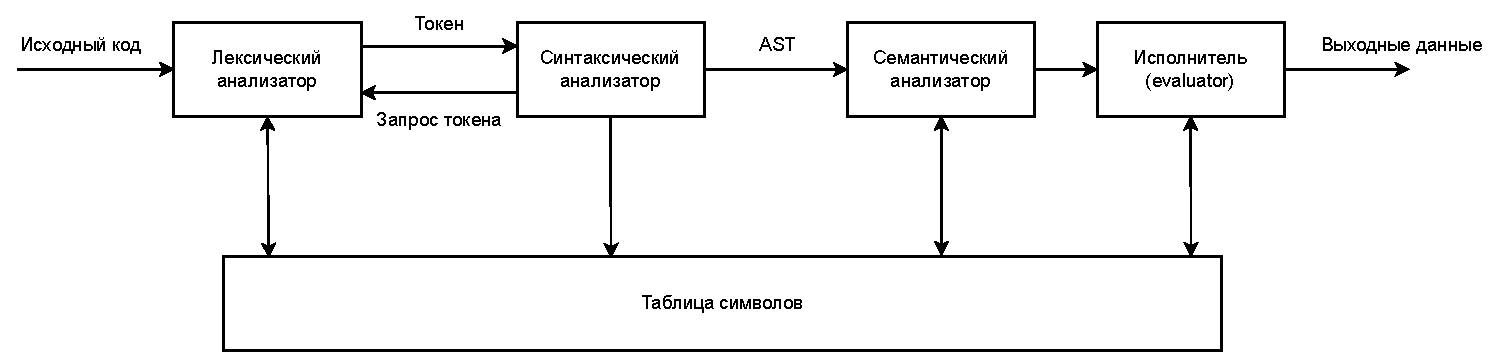
\includegraphics[width=1.0\textwidth]{structures/full_interpreter_struct.pdf}
	\caption{Обобщенная структура интерпретатора}
	\label{f:full_interpreter_struct}
\end{figure}

Для решения поставленной задачи, в первую очередь, необходимо в соответствии с указанными требованиями
разработать грамматику предметно-ориентированного языка и спроектировать обобщенную структуру программы интерпретатора.

\input{pages/content/structures/grammar.tex}
\input{pages/content/structures/lexical_analyzer.tex}
\input{pages/content/structures/parser.tex}
\input{pages/content/structures/semantic_analyzer.tex}
\newpage

\section{Программная реализация}

В данном разделе представлено описание выбранных инструментов разработки для решения поставленной задачи. 
Описана программная реализация модуля интерпретации предметно-ориентированного языка.
Рассмотрены детали реализации его основных структурных частей.
Также выполнено тестирование основных функций программы.

\subsection{Выбор инструментов разработки}

В качестве языка программирования для разработки был выбран Go.

Go (Golang) -- это компилируемый многопоточный язык программирования с открытым исходным кодом, разработанный компанией Google \refref{ref:golang}.

Выбор данного языка обусловлен совместимостью между разрабатываемым модулем и основной системой,
так как для реализации серверной части конструктора Telegram ботов так же был выбран язык Go.
Использование одного языка для всей системы гарантирует,
что модули будут легко интегрироваться друг с другом без необходимости создания сложных интерфейсов или адаптеров.

Язык Go имеет и другие положительные характеристики:
\begin{itemize}
    \item высокая производительность -- Go компилируется в машинный код, что обеспечивает его высокую скорость исполнения;
    \item безопасность типов -- строгая статическая типизация предотвращает множество ошибок на этапе компиляции;
    \item встроенная поддержка параллелизма -- в Go реализованы горутины и каналы -- встроенные механизмы для эффективной работы с параллельными задачами;
    \item расширяемость -- язык имеет встроенную систему управления модулями и широкую экосистему общедоступных библиотек.
\end{itemize}

Выбор языка программирования Go для реализации модуля интерпретации предметно-ориентированного языка конструктора Telegram ботов обоснован тем,
что он позволяет поддерживать единообразие кода, использовать его технические преимущества и соответствовать основным требованиям проекта.

\input{pages/content/implementation/lexer.tex}
\input{pages/content/implementation/parser.tex}
\input{pages/content/implementation/semantic_analyzer.tex}
\input{pages/content/implementation/evaluator.tex}
\input{pages/content/implementation/testing.tex}

\section*{Вывод}

В данном разделе на основании разработанных архитектурно-структурных решениях и алгоритмах функционирования выполнена программная реализация модуля интерпретации предметно-ориентированного языка.
С помощью выбранных инструментов разработки выполнена программная реализация лексического анализатора, синтаксического анализатора, семантического анализатора и исполнителя.

Также на базе встроенной в среду выполнения Go утилиты <<go test>> были реализованы юнит-тесты, охватывающие большинство функций модуля интерпретации.
\newpage

\csection{Заключение}

В ходе выполнения выпускной квалификационной работы выполнена разработка предметно-ориентированного языка для конструктора Telegram ботов и интерпретатора для него.
Основной целью проекта было расширение функциональных возможностей визуального конструктора Telegram ботов.
Благодаря использованию DSL можно более гибко настроить логику работы бота и предоставить пользователю платформы возможность построения сложных, уникальных ботов,
которых было бы невозможно или затруднительно построить с использованием только базового набора компонентов визуального конструктора.

На основе анализа предметной области и определения основных функциональных возможностей предметно-ориентированного языка было сформировано расширенное технического задание,
определяющее требования к разрабатываемому продукту.

Исходя из требований технического задания первоочередной задачей было разработать и описать грамматику предметно-ориентированного языка.
Для описания формальной грамматики была выбрана расширенная форма Бэкуса-Наура.

Была выполнена разработка архитектурно-структурных решений и алгоритмов функционирования каждой составляющей части модуля интерпретации,
а именно лексического, синтаксического, семантического анализаторов и исполнителя инструкций предметно-ориентированного языка.
Также описан программный интерфейс интеграции модуля с серверной частью конструктора.

На этапе программной реализации были выполнено кодирование анализаторов и исполнителя
в соответствии с разработанными алгоритмами функционирования с помощью выбранных инструментов разработки.
Кроме этого было осуществлено модульное тестирование разработанной программы.

Разработанный предметно-ориентированный язык позволяет расширить функциональные возможности конструктора Telegram ботов.
\docappendix{Листинг кода}

\begin{lstlisting}
var a = 1;
var b = 10;
var c = 123;
var d = a + b + c;

some_function(a, b, c);
\end{lstlisting}


\docappendix{Авторская справка}
\input{pages/authornote.example.tex}

\docappendix[справочное]{Какое-то справочное приложение}


Содержимое приложения

% \newpage

\csection{Библиографический список}

\begin{references}
	\item\label{ref:num-methods} Бахвалов Н.С., Жидков Н.П., Кобельников Г.М.
	Численные методы [Текст] – 4-е изд. – М:. БИНОМ. Лаборатория
	знаний, 2006. – 636 с.: ил.
	\item Безрученко Б.П., Смирнов Д.А.
	Статистическое моделирование по временным рядам [Электронный ресурс]
	Cарат. отд-ние Ин-та радиотехники и электроники РАН.
	– Электрон. дан. – Саратов, 2000. – Режим доступа:
	http://www.masters.donntu.edu.ua/2012/fknt/dorosh/library/article4.pdf,
	свободный. - Загл. с экрана.
	\item\label{ref:time-series-analysis} Бокс Дж., Дженкинс Г. Анализ временных рядов.
	Прогноз и управление [Текст]. - М.: Мир, 1974.
\end{references}

}

}

}

% Устанавливаем главную рамку для одной страницы
\tocloftpagestyle{mainframe}

% Устанавливаем рамку страниц, которая будет отрисовываться после главной
\pagestyle{pageframe}

% Меняем размер нижнего отступа до текста, чтобы текст до рамки страниц был 10mm.
% Рамка страниц имеет меньшую высоту содержимого нижней таблицы.
\addtolength{\textheight}{+25mm}
% Устанавливаем "Содержание", включающее в себя описание разделов документа
\tableofcontents\newpage

% Подключаем содержимое документа
\IfFileExists{./pages/content.tex} {
	% Пример файла содержимого документа
% Измените подключаемые файлы в зависимости от вашей структуры документа


\csection{Введение}

В современном мире все больше обретают популярность сервисы
визуального конструирования приложений.

Конструктор позволяет широкому кругу пользователей создавать программные продукты с помощью визуального редактора.
Пользователи могут выстраивать логику работы приложения просто перетаскивая визуальные блоки.
Это значительно упрощает разработку и делает её доступной даже для тех, кто не имеет глубоких знаний в программировании.
Однако функциональные возможности такого подхода к построению приложений ограничены и
их зачастую недостаточно для реализации сложных, специфичных программных продуктов.

Расширение возможностей платформы визуального конструктора возможно
за счёт использования предметно-ориентированного языка программирования.
С помощью написания инструкций на данном языке, пользователи  могут гибко задавать логику
работы разрабатываемого приложения.

\pagebreak


\section{Анализ предметной области}

В данном разделе проводится анализ предметной области,
который позволит обосновать актуальность разработки проекта,
приводятся ключевые требования и особенности конструкций,
которые должны быть реализованы в предметно-ориентированном языке визуального конструктора Telegram ботов.

\subsection{Актуальность разработки}

Боты в Telegram являются его популярной особенностью.
С их помощью пользователи могут в интуитивно понятной форме выполнять различные действия, не выходя из мессенджера Telegram.

Боты могут обладать различным функционалом и использоваться в различных сферах, например:
\begin{itemize}
    \item боты для общения с клиентами;
    \item техническая поддержка;
    \item продажа товаров и услуг;
    \item образовательные боты;
    \item боты для знакомств и общения;
    \item развлечения;
    \item утилиты и интрументы.
\end{itemize}

Боты имеют множетство плюсов как для пользователей, так и для их владельцев, например некоторые из них:
\begin{itemize}
    \item замена мобильного приложения;
    \item удобство использования, интерактивное взаимодействие;
    \item интеграция с другими системами;
    \item снижение затрат;
    \item круглосуточный доступ.
\end{itemize}

С ростом популярности ботов на рынке стали появляться визуальные конструкторы Telegram ботов --
решения для разработки и запуска ботов ботов с минимальным написанием программного кода или совсем без него. 

Визуальным конструктором называется NoCode/LowCode инструмент,
предназначенный для быстрого создания приложений без обязательного знания языков программирования общего назначения.
Иными словами, весь процесс разработки -- это взаимодействие с визуальными компонентами платформы,
с помощью которых выстраивается логика работы приложения.
За счет этого конструкторы значительно упрощают и удешевляют разработку и запуск программных продуктов.
Ведь не все обладают знаниями и навыками программирования с использованием языков общего назначения, достаточными для создания даже простых программ.
Кроме того, при наличии конструктора нет необходимости разрабатывать каждый раз отдельное приложение для выполнения типовых задач,
так как конструктор предоставляет необходимый набор инструментов для быстрого создания прототипа \refref{ref:nolowcode}.

Конструкторы имеют некоторые ограничения, например, при их использовании нельзя выйти за рамки возможностей самого конструктора,
а при выходе нового функционала Telegram Bot API,
владельцам платформы визуального конструирования ботов потребуется некоторые время на реализацию поддержки новых методов.

Однако использование только визуальных инструментов накладывает некоторые функциональные ограничения.
Обычно количество предоставляемых конструктором компонентов невелико и каждый из них способен выполнять только некоторую небольшую функцию, например отправить сообщение.
Это значительно ограничивает возможности пользователя в создании уникальных ботов.
Чтобы создание Telegram бота было более гибким, в систему можно интегрировать предметно-ориентированный язык программирования,
направленный на расширение функциональных возможностей визуального конструктора.
В отличие от визуальных блоков – язык позволяет пользователям сервиса гибко описывать логику работы бота.

Предметно-ориентированный язык (domain-specific language, DSL) -- это компьютерный язык, специализированный для конкретной предметной области применения \refref{ref:dsl}.
Противоположностью DSL являются языки общего назначения, такие как C++, Python, Go и т.д.

Примеры предметно-ориентированных языков:
\begin{itemize}
    \item язык запросов SQL -- применяется при работе с базами данных;
    \item shell-скрипты;
    \item HTML -- язык разметки пользовательского веб-интерфейса;
    \item CSS -- каскадные таблицы стилей, описывающие внешний вид веб-страницы.
\end{itemize}

Предметно-ориентированные языка можно разделить на две группы по способу представления конструкций \refref{ref:dsl_classification}:
\begin{enumerate}
    \item текстовые DSL -- текстовая форма, по аналогии с языками общего назначения;
    \item визуальные DSL -- формирование конструкций выполняется в графическом виде.
\end{enumerate}

Визуальные DSL получили большее распространение, поскольку графическое представление информации обладает большей наглядностью.

Также DSL делятся на два типа: внутренние и внешние.

Внутренние языки опираются на язык общего назначения, являются его часть и дополняют его.
Синтаксис такого DSL не может нарушать синтаксис базового языка.

Внешние DSL являются самостоятельными языками, имеют свой синтаксис и семантику.
Для успешного запуска они имеют свой компилятор или интерпретатор.

DSL разрабатываются с учетом особенностей предметной области,
благодаря чему являются менее избыточными по сравнению с языками общего назначения и более понятными для специалистов данной области.
Также предметно-ориентированные языки позволяют работать на более высоком уровне абстракции,
что увеличивает эффективность решения поставленных задач и снижает необходимость в изучении универсальных языков.
DSL языки легче изучать, учитывая их ограниченную область применения.

Помимо приведённых положительных аспектов предметно-ориентированных языков, они имеют некоторые недостатки.
DSL по сравнению с языками общего назначения имеют ограниченные возможности, например, малое разнообразие алгоритмов и структур данных.
Кроме того, разработка и внедрение предметно-ориентированного языка может привести к значительным тратам временных и финансовых ресурсов.

\subsection{Расширенное техническое задание}

В данном разделе представлено техническое задание на разработку предметно-ориентированного языка для конструктора Telegram ботов.

\subsubsection{Основание для разработки}

Программа разрабатывается на основе учебного плана кафедры
<<Электронные вычислительные машины>> по направлению 09.03.01.



\subsubsection{Цель и задача разработки}

Целью разработки является создание языка для расширения
функциональных возможностей визуального конструктора.

Задача разработки -- проектирование и разработки программного продукта по расширению функциональных возможностей визуального конструктора
на базе предметно-ориентированного языка. 



\subsubsection{Краткая характеристика области применения}

Программный продукт предоставляет пользователям возможность более гибкого создания приложений в среде визуального построения Telegram ботов.



\subsubsection{Назначение разработки}

Функциональным назначением является интерпретация кода предметно-ориентированного языка, написанного пользователем визуального конструктора.

Программа-интерпретатор является модулем визуального конструктора и эксплуатируется как его составная часть.
Особые требования к конечному пользователю не предъявляются.



\subsubsection{Требования к программному продукту}

Конструктор ботов делится на клиентскую и серверную части.
Серверная часть реализует основной функционал конструктора и логику его работы,
а так же предоставляет API интерфейс для клиентской части.
Клиентская часть предоставляет собой тонкий клиент в виде пользовательский веб-интерфейса.

Предметно-оринетированный язык должен быть выполнен в виде подключаемого модуля к серверной части платформы.
Модуль должен иметь программный интерфейс для запуска интерпретации кода предметно-оринетированного языка и возврата результата.
Помимо передачи кода на интерпретацию необходимо предусмотреть возможность передачи значений внешних переменных, используемых в передаваемом коде.

На клиентской части платформы должен быть реализован визуальный компонент,
позволяющий пользователю конструктора писать и редактировать код на предметно-оринтированном языке
и указывать внешние переменные, необходимые для успешного запуска кода.

Предметно-оринетированный язык конструктора должен обладать обозначенными ниже характеристиками.

Ключевые конструкции языка: переменные, ветвления, функции.

Поддерживаемые простые типы данных: строки, числа, булевы значения, <<Null>>.

Поддерживаемые составные типы данных: массив, хэш-карта.

Набор возможных операций языка:
\begin{itemize}
	\item арифметические операции: сложение, вычитание, умножение, деление, операция нахождение остатка от деления;
	\item логические операции: конъюнкция, дизъюнкция, отрицание;
	\item операции сравнения: равно, не равно, больше, меньше, больше или равно, меньше или равно;
	\item управляющие операции;
	\item вызов функций.
\end{itemize}

Интерпретатор предметно-ориентированного языка должен поддерживать все вышеперечисленные конструкции.

В задачи интерпретатора входит выполнение следующих этапов:
\begin{itemize}
	\item лексический анализ;
	\item синтаксический анализ;
	\item семантический анализ;
	\item исполнение операций;
\end{itemize}

Исходными данными является код программы на предметно-ориентированном языке.

Выходными данными является значение, полученное в результате успешного исполнения кода.

В случае возникновения ошибки на каком-либо из этапов интерпретации программа должна возвращать человекочитаемую ошибку.



\subsubsection{Требования к надежности}

Программа должна функционировать в соответствии с заданными требованиями при отсутствии сбоев технических средств.


\section*{Вывод}

В данном разделе был проведен анализ предметной области, в результате чего было определено,
что визуальные конструкторы значительно упрощают процесс создания и запуска Telegram ботов,
однако, они имеет функциональные ограничения, которые препятствуют разработке продукта со сложной логикой работы.
Предметно-ориентированный язык позволяет расширить возможности визуального конструктора и создавать уникальных ботов,
в соответствии с пользовательскими потребностями.

Также было рассмотрено расширенное техническое задание,
в котором были определены цели и задачи разработки и основные требования к разрабатываемому программному продукту.

Основываясь на этом можно приступить к разработке предметно-ориентированного языка для визуального конструктора Telegram ботов,
так как рассмотренная проблема является актуальной.
\newpage

\section{Разработка архитектурно-структурных решений}

Выполнение кода предметно-ориентированного языка осуществляется за счет интерпретатора,
который должен быть спроектирован в виде модуля, подключаемого к серверной части конструктора Telegram ботов.

Обобщенная модульная структура серверной части конструктора представлена на рисунке~\ref{f:modules_server_struct}.

\begin{figure}[ht]
	\centering
	\vspace{\toppaddingoffigure}
	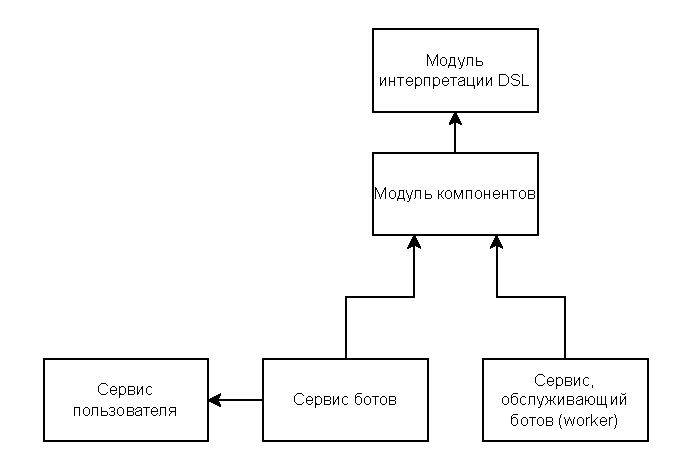
\includegraphics[width=0.7\textwidth]{structures/modules_server_struct.pdf}
	\caption{Модульная структура серверной части конструктора}
	\label{f:modules_server_struct}
\end{figure}

Сервис ботов отвечает за управление состоянием бота и редактирование его компонентной структуры.
Сервис ботов зависит от сервиса пользователей, который предоставляет первому методы для авторизации пользователя.
Также сервис ботов зависит от модуля компонентов, который описывает структуры компонентов и реализует их логику выполнения.

Обслуживающий сервис отвечает за логику работы бота. 
Он выполняет обработку запроса к боту от пользователя Telegram.
В соответствии с разработанной компонентной структурой бота, обслуживающий сервис вызывает методы модуля компонентов для запуска их логики выполнения.

Одним из компонентов является компонент выполнения кода на предметно-ориентированном языке.
Отсюда, модуль компонентов зависит от модуля интерпретации предметно-ориентированного языка.
При запуске компонента выполнения DSL кода, выполняется вызов функции выполнения кода из модуля интерпретации.

Таким образом, в данном проекте для возможности интеграции с серверной частью конструктора Telegram ботов необходимо реализовать программный интерфейс,
который бы предоставлял возможность передачи кода и значений внешних переменных, интерпретатору предметно-ориентированного языка.

Работа интерпретатора состоит из последовательного выполнения следующих этапов:
\begin{enumerate}
	\item лексический анализ;
	\item синтаксический анализ;
	\item семантический анализ;
	\item исполнение команд.
\end{enumerate}

Обобщенная структура интерпретатора представлена на рисунке~\ref{f:full_interpreter_struct}.

\begin{figure}[ht]
	\centering
	\vspace{\toppaddingoffigure}
	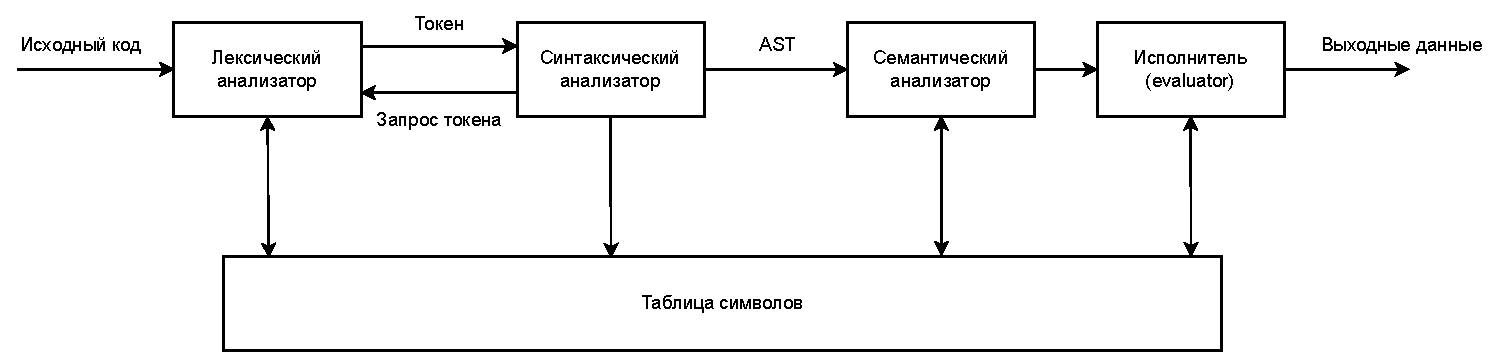
\includegraphics[width=1.0\textwidth]{structures/full_interpreter_struct.pdf}
	\caption{Обобщенная структура интерпретатора}
	\label{f:full_interpreter_struct}
\end{figure}

Для решения поставленной задачи, в первую очередь, необходимо в соответствии с указанными требованиями
разработать грамматику предметно-ориентированного языка и спроектировать обобщенную структуру программы интерпретатора.

\subsection{Разработка грамматики языка}

Описание языка программирования основывается на теории формальных языков.
В данном разделе проводится разработка формальной грамматики языка и её описание.


\subsubsection{Способы задания языков}

Для задания языка можно воспользоваться следующими методами:

\begin{enumerate}
    \item перечислить все цепочки языка;
    \item указать способ порождения цепочек;
    \item определить метод распознавания допустимых цепочек.
\end{enumerate}

Перечисление всех цепочек языка возможно в исключительных случаях, например,
когда для управления некоторой системой достаточно двух-трех команд.

Механизм порождения цепочек предполагает использование формальной порождающей грамматики.

Формальная порождающая грамматика -- это математическая система, описывающая правила построения цепочек некоторого (формального) языка \refref{ref:grammar}.

Распознавание допустимых цепочек осуществляется с помощью некоторого логического устройства -- распознавателя.
На вход распознавателя подается цепочка, а на выходе образуется логическое значение <<истина>> в случае принадлежности цепочки языку
и <<ложь>>, если цепочка языку не принадлежит.
Распознаватели строятся на основе теорий конечных автоматов и автоматов с магазинной памятью.

Методы порождения и распознавания тесно связаны.
Механизм порождения обычно используется при описании языка, а распознаватель при его реализации, т.е. в трансляторе.

Описать синтаксис языков программирования можно несколькими способами, например, такими как формы Бэкуса-Наура, диаграммы Вирта и другими.
Это методы задают правила вывода, определяющие возможные конструкции цепочек языка.
В данном проекте для описания грамматики языка используется расширенная форма Бэкуса-Наура (РБНФ).



\subsubsection{Применение расширенной формы Бэкуса-Наура для описания формальной грамматики языка}

Расширенная форма Бэкуса-Наура – формальная система определения синтаксиса,
в которой одни синтаксические категории последовательно определяются через другие.
Используется для описания контекстно-свободных грамматик \refref{ref:rbnf}.

Формальная грамматика задаётся четвёркой вида:

\(G = (V_T, V_N, P, S)\),

где \(V_T\) -- множество терминальных символов грамматики – конечные
элементы языка, не разбирающиеся на более мелкие составляющие в рамках
синтаксического анализа, например ключевые слова, цифры, буквы
латинского алфавита.

\(V_N\) -- конечное множество нетерминальных символов – элементов грамматики, имеющих собственные имена и структуру.
Каждый нетерминальный символ состоит из одного или более терминальных и/или нетерминальных символов.

\(P\) -- множество правил вывода грамматики.

\(S\) -- начальный символ грамматики, \(S \in V_N\) \refref{ref:grammar}.

РБНФ является одним из способов представления формальных грамматик.
РБНФ состоит из множества правил вывода, каждое из которых определяет синтаксис некоторой конструкции языка.

Некоторые основные конструкции РБНФ:

\begin{itemize}
    \item A, B -- конкатенация элементов;
    \item A | B -- выбор (A или B);
    \item {[A]} -- элемент в квадратных скобках может отсутствовать (аналог - <<?>>);
    \item \{A\} -- повторение элемента 0 или более раз (аналог - <<*>>);
    \item (A B) -- группировка элементов;
    \item (* … *) – комментарий;
    \item <<;>> – отмечает окончание правила (аналог - <<.>>).
\end{itemize}

Кроме того, в качестве синтаксического сахара могут использоваться следующие символы:

\begin{itemize}
    \item <<*>> - предыдущий элемент может встречаться 0 или более раз;
    \item <<?>> - предыдущий элемент является необязательным (присутствует 0 или 1 раз);
    \item <<+>> - предыдущий элемент встречается 1 или более раз.
\end{itemize}

В соответствии с данными правилами описание синтаксиса предметно-ориентированного языка будет выглядеть следующим образом:

(* Точка входа *)

Program = Statement+ \\


(* Основные конструкции *)

Statement = AssignStmt | FunctionDecl | ExpressionStmt | ReturnStmt | BlockStmt | IfStmt .

ExpressionStmt = Expression . \\

AssignStmt = Identifier assign\_op Expression .

ReturnStmt = "{}return"{} [Expression] .

BlockStmt = "{}\{"{} StatementList "{}\}" .

StatementList = \{ Statement "{};"{} \} .

IfStmt = "{}if("{} [Expression] "{})"{} BlockStmt ["{}else"{} BlockStmt] . \\


(* Выражения *)

Expression = UnaryExpr | Expression binary\_op Expression . 

UnaryExpr = PrimaryExpr | unary\_op UnaryExpr . \\

PrimaryExpr = Operand | PrimaryExpr Index | CallExpr .

Index = "{}["{} Expression "{}]"{} .

ExpressionList = Expression \{ "{},"{} Expression \} . \\


(* Определение структуры функции *)

FunctionDecl = "{}fn("{} [ParameterList] "{})"{} BlockStmt .

ParameterList = Identifier \{ "{},"{} Identifier \} .

Arguments = "{}("{} [ ExpressionList ] "{})"{} .

CallExpr = Identifier Arguments . \\


(* Массив *)

Array = "{}["{} [ ExpressionList ] "{}]"{} . \\


(* Хэш-карта *)

Key = stringLiteral | intLiteral | Identifier | Expression .

KeyedElement  = [ Key "{}:"{} Expression ] .

Map = "{}\{"{} KeyedElement \{ "{},"{} KeyedElement \} "{}\}"{} . \\


Identifier = (letter | "{}\_"{}) { letter | "{}\_"{} | digit } .

Operand = Literal | "{}("{} Expression "{})"{} .

Literal = intLiteral | stringLiteral | Array | Map .

intLiteral = digit \{ digit \} .

stringLiteral = << "{} >> \{ ascii\_char \} << "{} >> . \\


(* Операторы *)

binary\_op = "{}||"{} | "{}\&\&"{} | rel\_op | add\_op | mul\_op .

rel\_op = "{}=="{} | "{}!="{} | \"{}<\"{} | "{}<="{} | "{}>"{} | "{}>="{} .

add\_op = "{}+"{} | "{}-"{} .

mul\_op = "{}*"{} | "{}/"{} | "{}\%"{} .

assign\_op = "{}="{} .

unary\_op = "{}-"{} | "{}!"{} . \\


(* Примитивы (цифры, буквы) *)

digit = "{}0"{} ... "{}9"{} .

letter = "{}A"{} ... "{}Z"{} | "{}a"{} ... "{}z"{} .

ascii\_char = ascii character . \\

Начальное состояние, с которого начинается разбор -- Program.

% В данном разделе была разработана и описана с помощью расширенной формы Бэкуса-Наура формальная грамматика предметно-ориентированного языка.
\subsection{Разработка лексического анализатора}

% В данном разделе необходимо выполнить разработку алгоритмов функционирования лексического анализатора.

Лексический анализ – процесс разбора входной последовательности символов на распознанные группы – лексемы.

Лексемой является структурная (минимальная значимая) единица языка, состоящая из элементарных символов языка и не содержащая в своём составе других структурных единиц языка.

В ходе выполнения лексического анализатора каждая лексема идентифицируется и преобразуется в токен.

Токен – экземпляр лексемы, представляющий собой пару «тип лексемы» и «значение».
«Тип» указывает на принадлежность лексемы к определенной категории, например, идентификатор, число и т.д., а «значение» содержит конкретные данные, соответствующие этой лексеме.

Категории токенов, которые используются в разрабатываемом предметно-ориентированном языке:
\begin{itemize}
    \item идентификаторы;
    \item числа;
    \item строки;
    \item разделители;
    \item операторы (арифметические, сравнения и т.д);
    \item скобки;
    \item специальные (конец входной последовательности и т.п)
    \item ключевые слова.
\end{itemize}

Полный список токенов с указанием категории и примерами лексем приведен в таблице~\ref{t:tokens}.

Процесс лексического анализа является первым шагов в трансляции исходного кода программы и формирует основу для следующих этапов,
таких как синтаксический анализ и построение абстрактного синтаксического дерева.

\clearpage

\begin{table}[h!]
    \Large
    \centering
    \begin{threeparttable}
        \caption{Токены с примерами}
        \label{t:tokens}
        \begin{tabularx}{\textwidth}{|X|c|c|}
            \hline
            Токен         & Категория      & Пример лексемы  \\
            \hline
            IDENT         & Идентификатор  & qwe             \\
            \hline
            INT           & Число          & 123             \\
            \hline
            STRING        & Строка         & «привет, hello» \\
            \hline
            ASSIGN        & Оператор       & =               \\
            \hline
            PLUS          & Оператор       & +               \\
            \hline
            MINUS         & Оператор       & -               \\
            \hline
            STAR          & Оператор       & *               \\
            \hline
            SLASH         & Оператор       & /               \\
            \hline
            EXCLAMINATION & Оператор       & !               \\
            \hline
            PERCENT       & Оператор       & \%              \\
            \hline
            EQ            & Оператор       & ==              \\
            \hline
            NEQ           & Оператор       & !=              \\
            \hline
            LEQ           & Оператор       & <=              \\
            \hline
            GEQ           & Оператор       & =>              \\
            \hline
            LT            & Оператор       & <               \\
            \hline
            GT            & Оператор       & >               \\
            \hline
            LAND          & Оператор       & \&\&            \\
            \hline
            LOR           & Оператор       & ||              \\
            \hline
            COMMA         & Разделитель    & ,               \\
            \hline
            SEMICOLON     & Разделитель    & ;               \\
            \hline
            LPAR          & Скобка         & (               \\
            \hline
            RPAR          & Скобка         & )               \\
            \hline
            LBRACE        & Скобка         & \{              \\
            \hline
            RBRACE        & Скобка         & \}              \\
            \hline
            LBRACKET      & Скобка         & [               \\
            \hline
            RBRACKET      & Скобка         & ]               \\
            \hline
            IF            & Ключевое слово & if              \\
            \hline
            ELSE          & Ключевое слово & else            \\
            \hline
            TRUE          & Ключевое слово & true            \\
            \hline
            FALSE         & Ключевое слово & false           \\
            \hline
            FUNC          & Ключевое слово & fn              \\
            \hline
            RETURN        & Ключевое слово & return          \\
            \hline
            ILLEGAL       & Специальный    & @               \\
            \hline
            EOF           & Специальный    & Конец файла     \\
            \hline
        \end{tabularx}
    \end{threeparttable}
    \vspace{\bottompaddingoftable}
\end{table}

Схема взаимодействия лексического и синтаксического анализаторов показана на рисунке~\ref{f:la_sa_struct}.

\begin{figure}[ht]
	\centering
	\vspace{\toppaddingoffigure}
	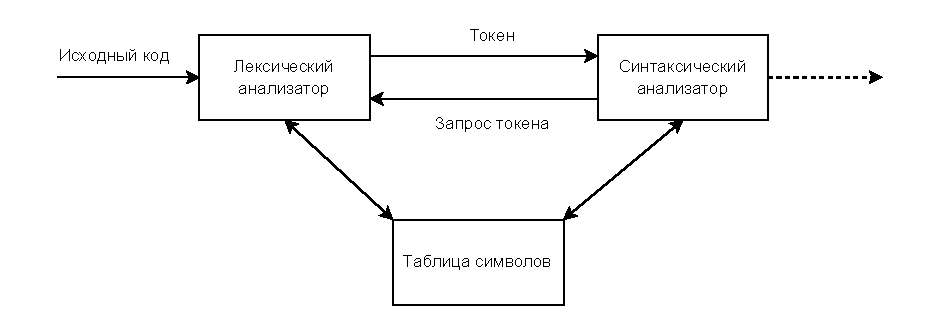
\includegraphics[width=0.9\textwidth]{structures/lexical_analyzer/la_sa_struct.pdf}
	\caption{Схема взаимодействия лексического и синтаксического анализаторов}
	\label{f:la_sa_struct}
\end{figure}

При запросе нового токена лексический анализатор считывает входной поток символов до точной идентификации следующего токена.

Процесс распознавания токенов из входного потока символов языка можно показать с помощью диаграмм переходов состояний.

На рисунке~\ref{f:dps_eq_assign} показана диаграмма для определения токенов «=» и «==».

\begin{figure}[ht]
	\centering
	\vspace{\toppaddingoffigure}
	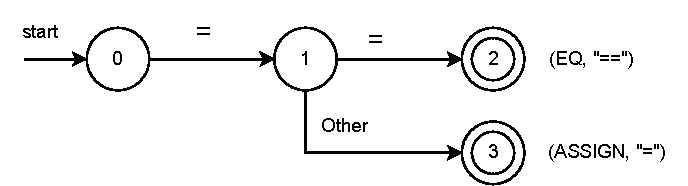
\includegraphics[width=0.9\textwidth]{structures/lexical_analyzer/dps_eq_assign.pdf}
	\caption{Диаграмма переходов для определения «=» и «==»}
	\label{f:dps_eq_assign}
\end{figure}

Работа начинается с состояния 0, в котором считывается следующий символ из входного потока.
Если полученный символ «=», то по дуге, помеченной «=» выполняется переход в состояние 1.
В состоянии 1 выполняется считывание следующего символа.
Если этот символ «=», выполняется переход в состояние 2 – заключительное состояние,
в котором найден токен «EQ», в том случае, если был получен символ отличный от «=»,
происходит переход по дуге «other» в состояние 3 с токеном «ASSIGN».

Диаграмма для распознавания целого числа представлена на рисунке~\ref{f:dps_int}.

\begin{figure}[ht]
	\centering
	\vspace{\toppaddingoffigure}
	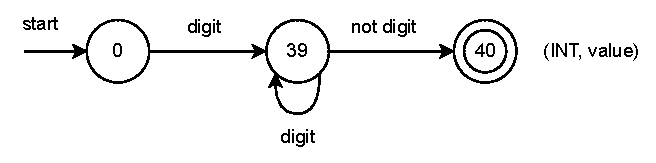
\includegraphics[width=0.9\textwidth]{structures/lexical_analyzer/dps_int.pdf}
	\caption{Диаграмма переходов для определения целого числа}
	\label{f:dps_int}
\end{figure}

При получении в начальном состоянии цифры, выполняется переход в состояние 39, в котором автомат находится до тех пор,
пока не получит на вход символ, отличный от цифры, при получении такого символа выполняется переход в конечное состояние 40.
По мере определения очередной цифры, она заносится в буфер.
В состоянии 40 возвращается токен INT и значение числа из буфера.

Считывание ключевых слов и идентификаторов показано с помощью диаграммы передов на рисунке~\ref{f:dps_ident_kw}.

Из начального состояния происходит переход в состояние 35, если была получена буква.
По аналогии с состоянием 39 выполняется циклическое считывание букв с занесением в буфер.
Если была получена не буква, выполняется переход в состояние 36, в котором проверяется принадлежность считанной строки к списку ключевых слов.
В случае, если считанная строка является ключевым словом, автомат переходит в завершающее состояние 37 в котором указывается тип токена для полученного ключевого слова и значение.
Если в состоянии 36 проверка показала, что строка на является ключевым словом, то выполняется переход в состояние 38 – определен идентификатор.

\begin{figure}[ht]
	\centering
	\vspace{\toppaddingoffigure}
	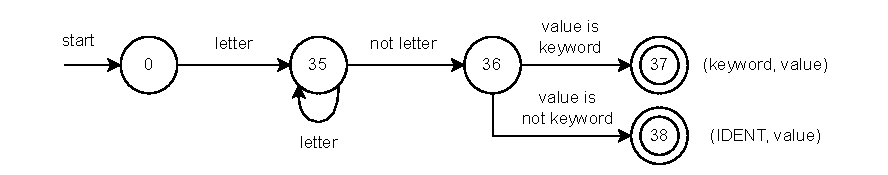
\includegraphics[width=0.9\textwidth]{structures/lexical_analyzer/dps_ident_kw.pdf}
	\caption{Диаграмма переходов для определения идентификаторов и ключевых слов}
	\label{f:dps_ident_kw}
\end{figure}

Полная диаграмма переходов состояний представлена на рисунке~\ref{f:full_dps}

Процесс распознавания токена начинается с начального состояния 0.
В зависимости от полученного символа выполняется переход в конкретное состояние.
Однако, если в начальном состоянии был получен символ, для которого нет дуги,
по которой он бы мог перейти в определенное для него состояние, выполняется переход по дуге «other» в состояние 42 с определением токена ILLEGAL.
После определения очередного токена в конечном состоянии, автомат начинает работу заново с начального состояния.
Считывание входного потока символов прекращается при поступлении нулевого символа (null character) с определением токена EOF.
Вместе с токеном, лексический анализатор возвращает его позицию в входном коде.

% В данном разделе была выполнена разработка структурных решений и алгоритмов функционирования лексического анализатора предметно-ориентированного языка.

\clearpage

\begin{figure}[h!]
	\centering
	\vspace{\toppaddingoffigure}
	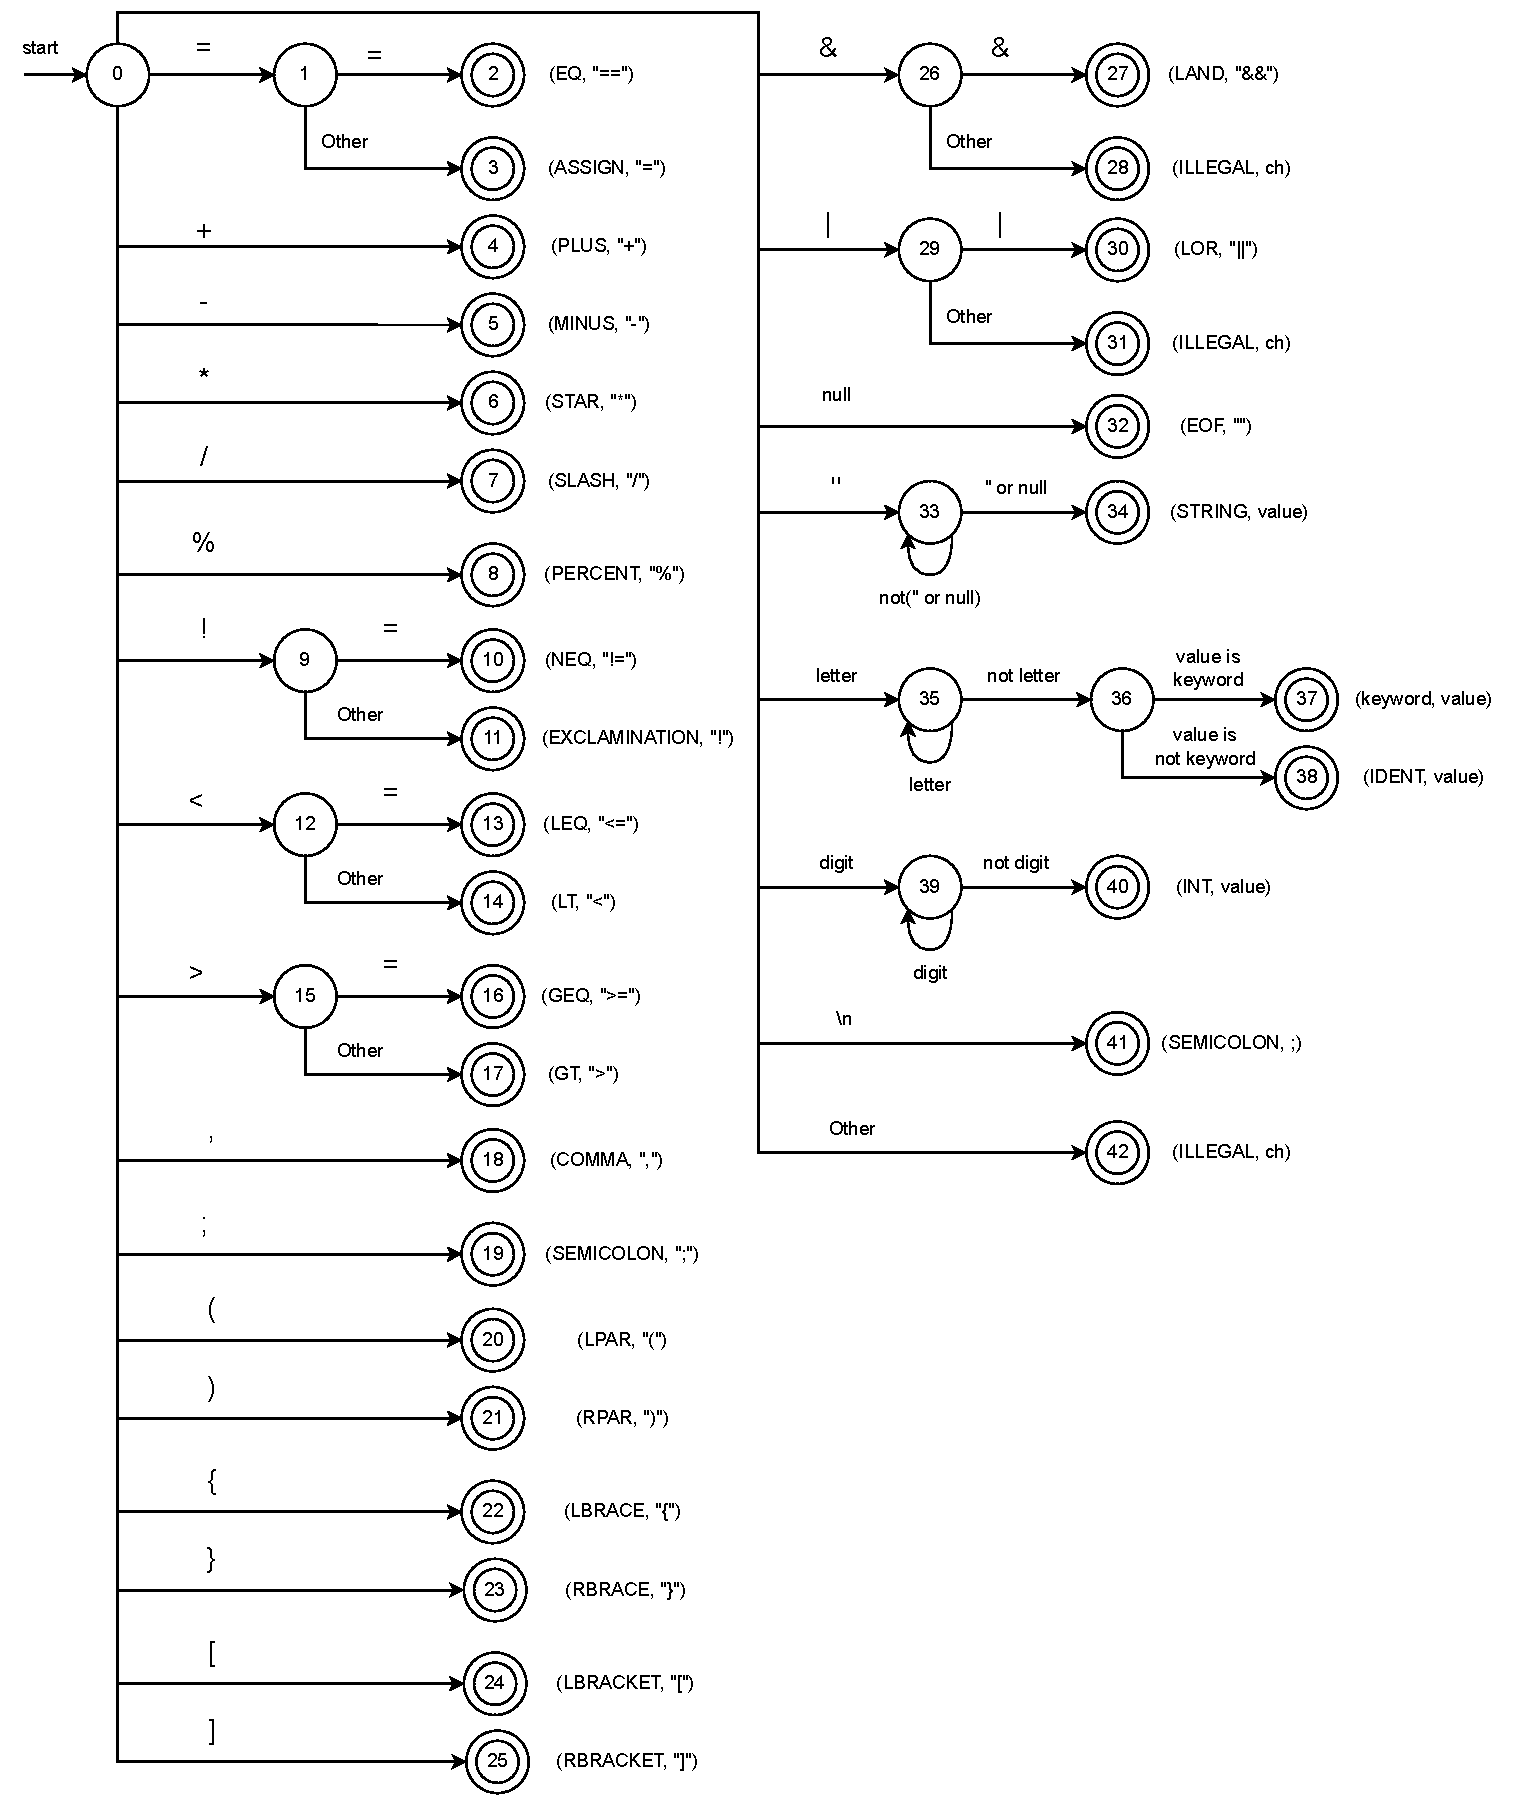
\includegraphics[width=1.0\textwidth]{structures/lexical_analyzer/full_dps.pdf}
	\caption{Полная диаграмма переходов состояний}
	\label{f:full_dps}
\end{figure}

\clearpage
\subsection{Разработка синтаксического анализатора}

% В данном разделе необходимо выполнить разработку алгоритмов функционирования синтаксического анализатора.

Синтаксический анализ – процесс сопоставления последовательности токенов с формальной грамматикой языка.
Результатом работы синтаксического анализатора является абстрактное синтаксическое дерево (AST),
которое отражает синтаксическую структуру входной последовательности и содержит всю необходимую информацию для дальнейших этапов работы транслятора.

В задачу синтаксического анализа входит поиск и выделение основных синтаксических конструкций текста входной программы,
установление типа и проверка правильности каждой синтаксической конструкции, а так же представление их в виде AST.

Существует два основных метода синтаксического анализа:

\begin{itemize}
    \item нисходящий;
    \item восходящий.
\end{itemize}

В данном проекте реализован нисходящий анализатор, работающий по методу рекурсивного спуска,
известный как парсер Пратта, который впервые описал Вон Пратт в статье «Нисходящий парсер с операторным предшествованием».

Этот метод основан на идее приоритета операторов и обработке различных уровней приоритета в выражениях.
В парсере Пратта каждый оператор имеет свой уровень приоритета.
Операторы с более высоким приоритетом связываются с операндами сильнее, чем операторы с более низким приоритетом.
Значения приоритетов для каждого оператора разрабатываемого предметно-ориентированного языка показаны в таблице~\ref{t:operator_priority}.

\clearpage

\begin{table}[h!]
    \Large
    \caption{Приоритеты операторов}
    \label{t:operator_priority}
    \centering
    \begin{tabularx}{\textwidth}{|c|X|}
        \hline
        Приоритет & Операторы             \\
        \hline
        0         & Минимальный приоритет \\
        \hline
        1         & =                     \\
        \hline
        2         & | |                   \\
        \hline
        3         & \&\&                  \\
        \hline
        4         & == !=                 \\
        \hline
        5         & < > <= >=             \\
        \hline
        6         & + -                   \\
        \hline
        7         & * / \%                \\
        \hline
        8         & -x or !x              \\
        \hline
        9         & (                     \\
        \hline
        10        & [                     \\
        \hline
    \end{tabularx}
    \vspace{\bottompaddingoftable}
\end{table}

Для примера работы приоритета операторов рассмотрим пример построения AST для арифметического выражения: $3 + 1 * 4 * 6 + 8$.
Диаграмма, показывающая рекурсивные вызовы для формирования выражений к приведенному примеру изображена на рисунке~\ref{f:priorities}.

\begin{figure}[ht]
	\centering
	\vspace{\toppaddingoffigure}
	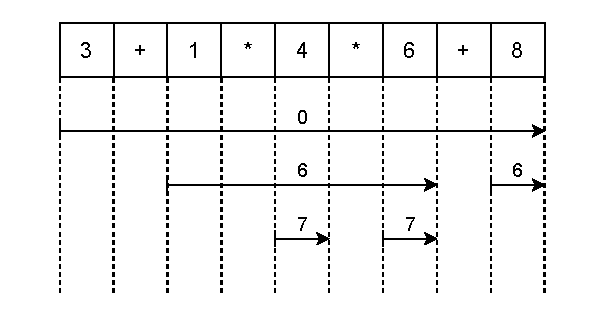
\includegraphics[width=0.7\textwidth]{structures/parser/priorities.pdf}
	\caption{Диаграмма рекурсивных вызовов}
	\label{f:priorities}
\end{figure}

Над стрелками обозначены приоритеты операторов, к которым относится эта стрелка.
В самом начале распознавания выражения значение приоритета равняется 0.
По мере обнаружения оператора, приоритет которого выше текущего алгоритм переходит на следующий уровень рекурсии.
По диаграмме видно, что справа от первого оператора «+» длинная стрелка с приоритетом 6, группирует члены умножения, так как операция умножения имеет больший приоритет, чем сложение.
Эта стрелка заканчивается перед последним «+», так как приоритет оператора, относящегося к этой стрелке не ниже приоритета последнего «+».
Другими словами, экземпляр выражения с более низким приоритетом ожидает результата формирования выражения с более высоким приоритетом.

Абстрактное синтаксическое дерево для данного примера приведено на рисунке~\ref{f:ast_example}.

\begin{figure}[ht]
	\centering
	\vspace{\toppaddingoffigure}
	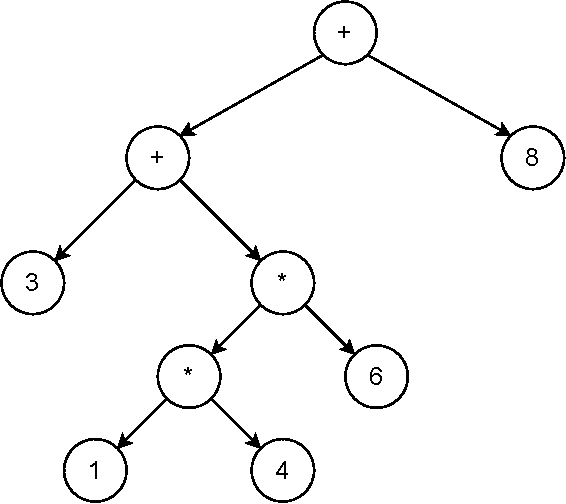
\includegraphics[width=0.7\textwidth]{structures/parser/ast_example.pdf}
	\caption{Абстрактное синтаксическое дерево}
	\label{f:ast_example}
\end{figure}

Некоторые схемы алгоритма построения абстрактного синтаксического дерева представлены на рисунках~\ref{f:parse_program}~-~\ref{f:parse_Expression}.

% В данном разделе была выполнена разработка структурных решений и алгоритмов функционирования синтаксического анализатора.

\clearpage

\begin{figure}[!htp]
	\centering
	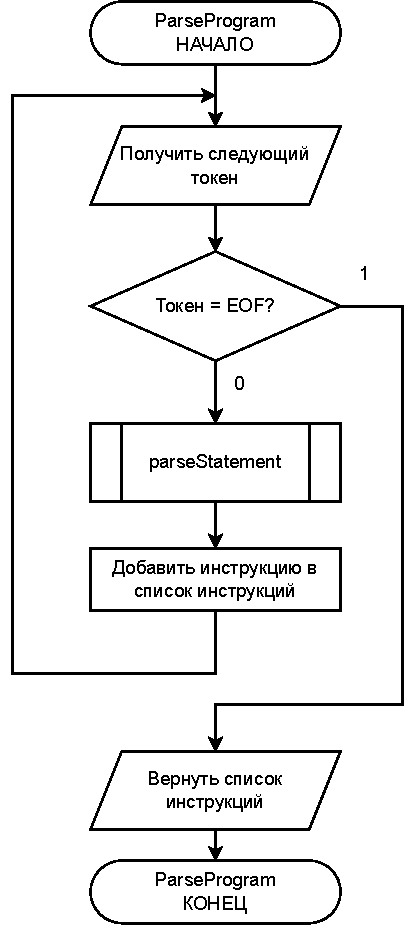
\includegraphics[width=0.5\textwidth]{structures/parser/parse_program.pdf}
	\caption{Схема алгоритма «ParseProgram»}
	\label{f:parse_program}
\end{figure}

\clearpage

\begin{figure}[!htp]
	\centering
	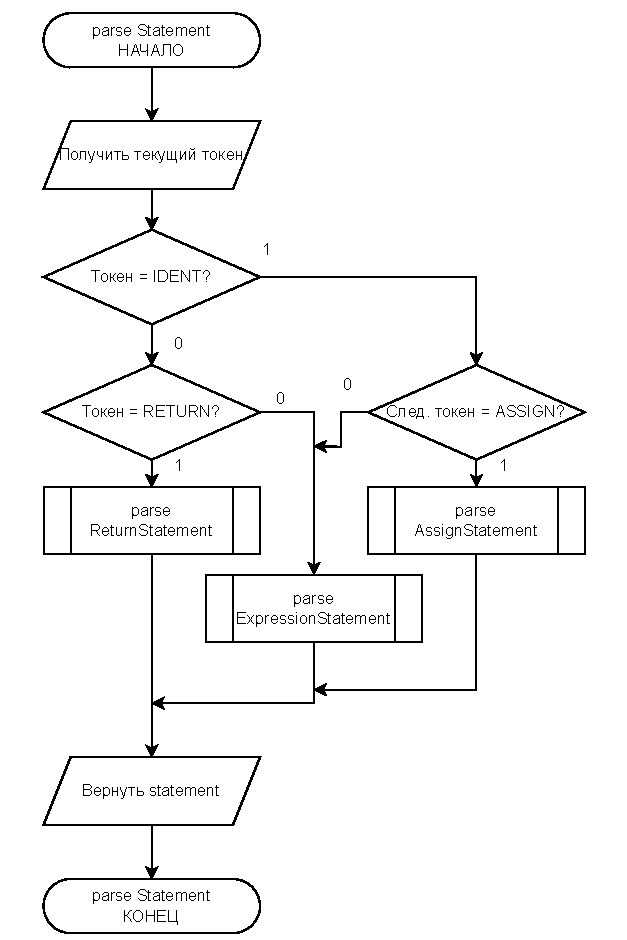
\includegraphics[width=0.7\textwidth]{structures/parser/parse_statement.pdf}
	\caption{Схема алгоритма «parseStatement»}
	\label{f:parse_statement}
\end{figure}

\clearpage

\begin{figure}[!htp]
	\centering
	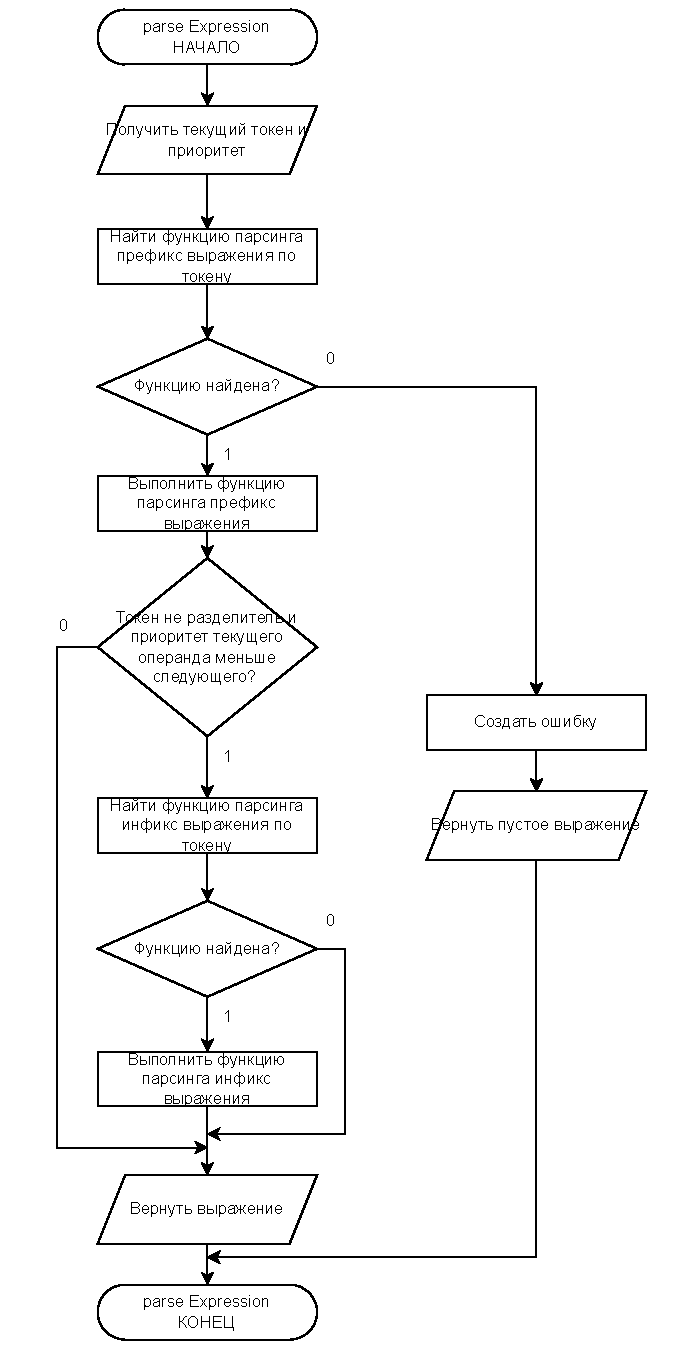
\includegraphics[width=0.60\textwidth]{structures/parser/parse_Expression.pdf}
	\caption{Схема алгоритма «parseExpression»}
	\label{f:parse_Expression}
\end{figure}

\clearpage


\subsection{Разработка семантического анализатора}

% В данном разделе необходимо выполнить разработку алгоритмов функционирования семантического анализатора.

Семантический анализ – это этап работы транслятора, вот время которого выполняется проверка текста исходной программы с точки зрения семантики языка.
В ходе семантического анализа выполняется такие операции, как проверка типов данных, правильность использования переменных, функций, выражений, а также обнаружение смысловых ошибок в коде.

Обобщенная модульная структура серверной части конструктора представлена на рисунке~\ref{f:modules_server_struct}.

Процесс семантического анализа выполняется после построения абстрактного синтаксического дерева синтаксическим анализатором.
Семантический анализ сгруппирован с этапом исполнения выражений.
Таким образом при одном проходе AST алгоритм выполняет проверку узла дерева на семантическую корректность и переход к его исполнению,
если не было обнаружено ошибок при семантическим анализе. В случае обнаружения семантической ошибки возвращается информация о ней,
а процесс интерпретации переход к следующему выражению.

На этапе проектирования семантического анализатора закладываются решения, которые лягут в основу принципов написания кода на разрабатываемом языке.
Например, на этапе построения семантического анализатора, нужно решить, как будет обрабатываться значение в условном выражении, не имеющее тип boolean.
Есть несколько вариантов обработки таких значений.
Один из них - всегда принимать данное значение за «false» и идти в соответствующую ветвь.
В ином случае, при обнаружении значения с типом, отличным от boolean необходимо вернуть ошибку и прекратить выполнение данного выражения.
В этом проекте будет использован второй вариант с возвратом ошибки.

Семантический анализатор принимает на вход элементы абстрактного синтаксического дерева.
После проверки семантической корректности выражения AST, следует его вычисление.
Результаты вычислений выражений, как промежуточные, так и окончательные необходимо каким-то образом представить в памяти.
Это необходимо в первую очередь для получения ранее вычисленных выражений и работы с ними.
В качестве примера можно рассмотреть код, представленный на рисунке~\ref{f:code_example_var}.

\begin{figure}[ht]
	\centering
	\vspace{\toppaddingoffigure}
	\begin{lstlisting}
X = 5;
X + 3
\end{lstlisting}
	\caption{Пример кода использования объявленной переменной}
	\label{f:code_example_var}
\end{figure}

В первой строке присваивается значение 5 переменной «X».
Затем выполняется выражение «X + 3».
Чтобы получить значение данного выражения нужно получить ранее вычисленное значение 5.
Для этого необходимо как-то сохранить его в памяти.

Решение данной задачи состоит в введении внутреннего представления вычисленных значений на время семантического анализа и этапа исполнения.
Примем некоторую объектную систему, состоящую из набора объектов, каждый из которых будет содержать информацию о представляемом им типе данных в предметно-ориентированном языке.

Каждый объект должен содержать информацию о значении представляемого им типа данных предметно-ориентированного языка.
Кроме этого, необходимо реализовать возможность определения того, какой тип данных предметно-ориентированного языка представляет объект, а также функционал получения строкового значения объекта.
Кроме этого, типы данных: целое число, строка и булево значение могут использоваться в виде ключей в хэш-карте.
Для этого необходимо специально для объектов, представляющих эти типы предусмотреть функцию вычисления хэш строки от их значения. 

Объектная система должна представлять все типы данных предметно-ориентированного языка, а именно:
целые числа, строки, булевы значения, массивы, хэш-карты.
Также необходимо ввести дополнительные объекты, представляющие семантические ошибки, значение «null», функции, операцию возврата значения из функции.

Объектная система может быть представлена в виде диаграммы классов.
Диаграмма классов представлена на рисунке~\ref{f:class_diagram}.

\clearpage

\begin{figure}[!htp]
	\centering
    \vspace{\toppaddingoffigure}
	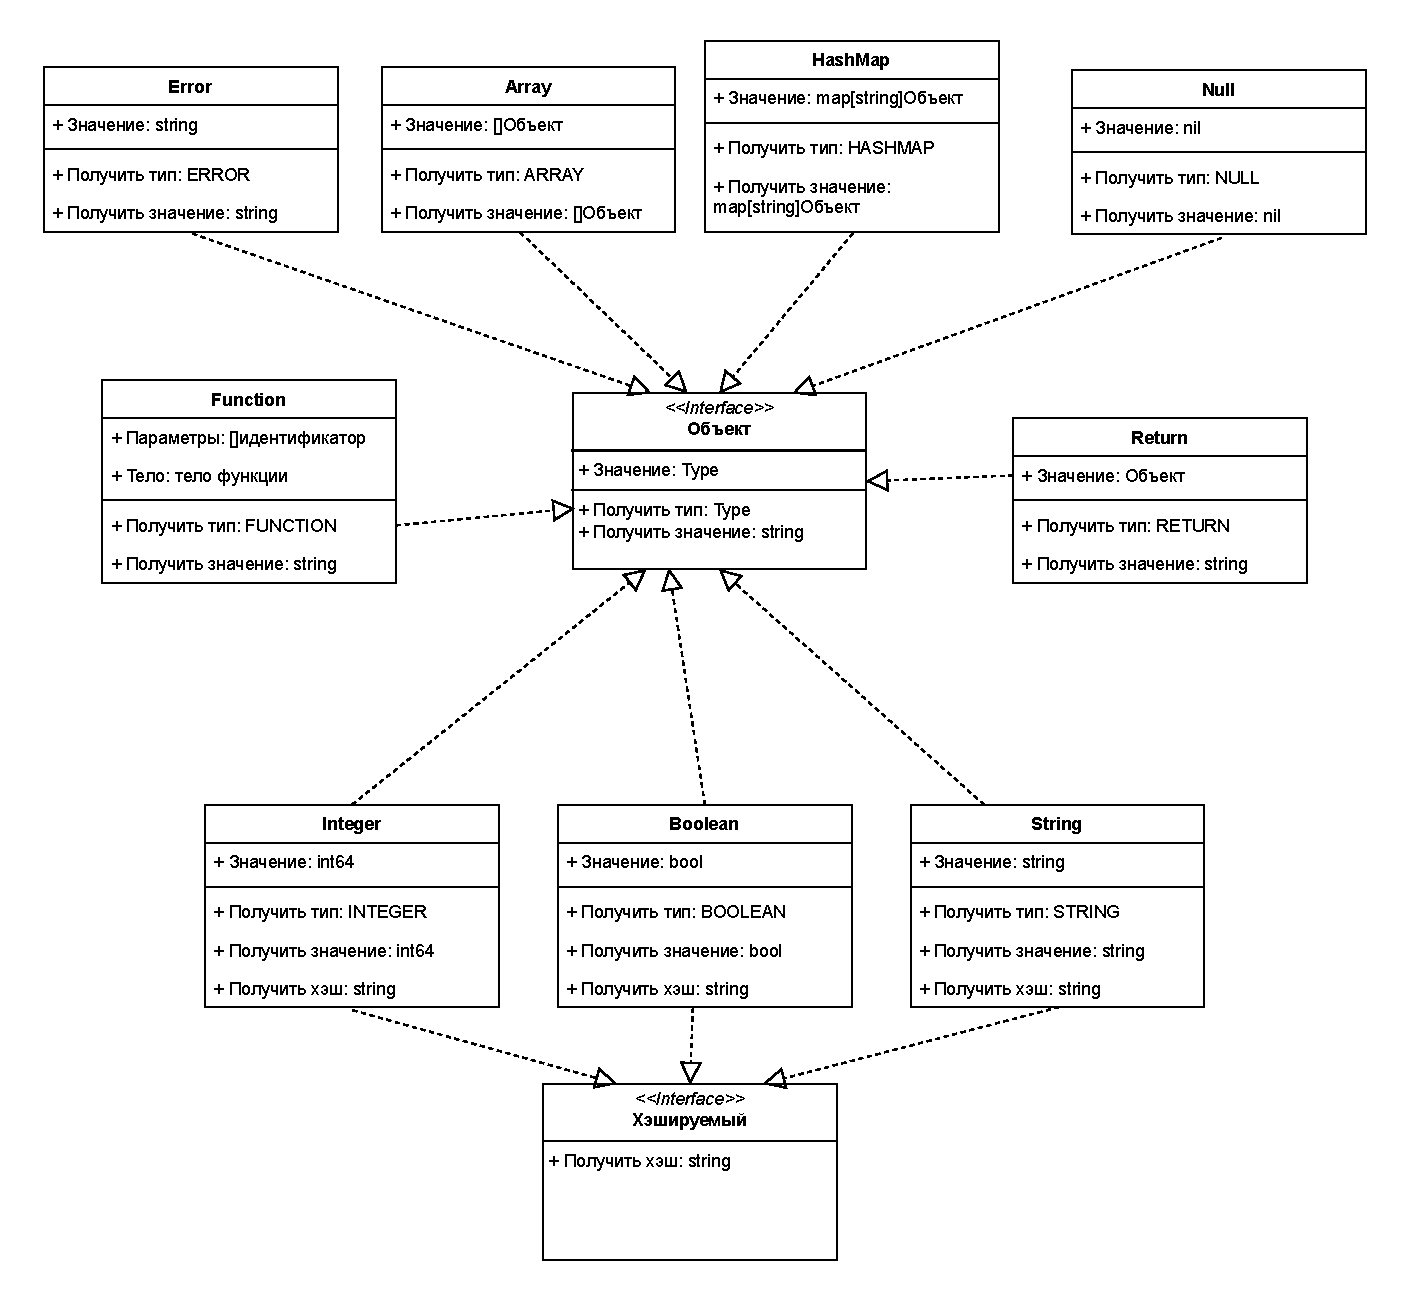
\includegraphics[width=1.0\textwidth]{structures/semantic_analyzer/class_diagram.pdf}
	\caption{Диаграмма классов}
	\label{f:class_diagram}
\end{figure}

В качестве примера работы алгоритма на рисунках~\ref{f:evalProgram}~-~\ref{f:semantic_index_expr} приведены схемы алгоритмов семантического анализа некоторых выражений.

% В данном разделе была выполнена разработка структурных решений и алгоритмов функционирования семантического анализатора.

\begin{figure}[!htp]
	\centering
	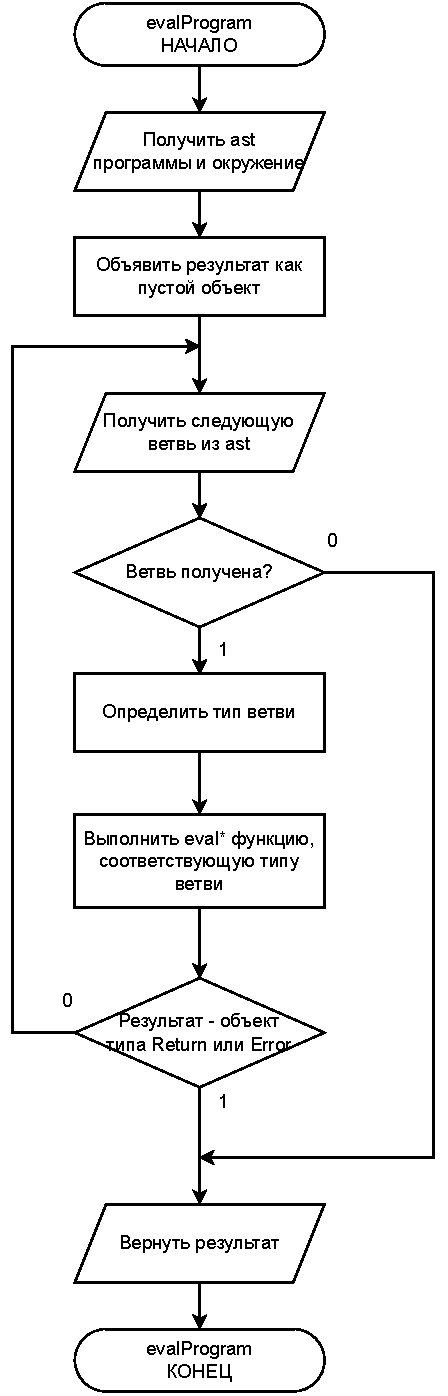
\includegraphics[width=0.4\textwidth]{structures/semantic_analyzer/semantic_Program.pdf}
	\caption{Схема алгоритма «evalProgram»}
	\label{f:evalProgram}
\end{figure}

\clearpage

\begin{figure}[!htp]
	\centering
	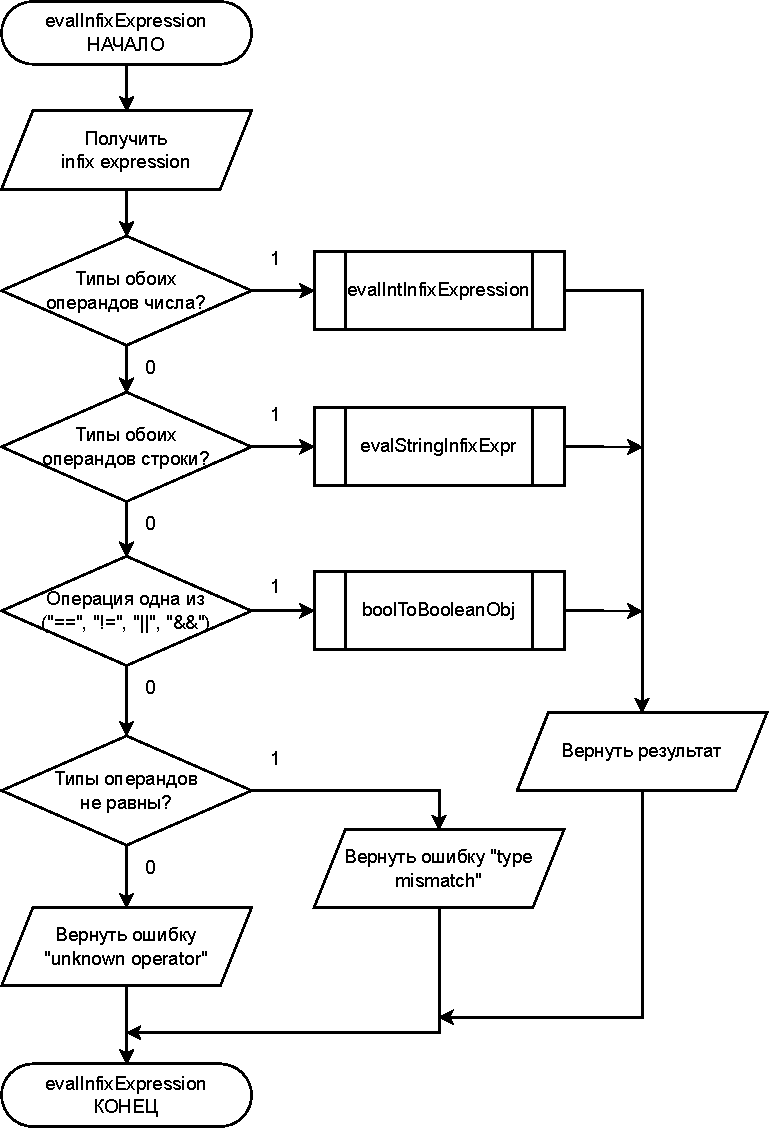
\includegraphics[width=0.9\textwidth]{structures/semantic_analyzer/semantic_infix_expr.pdf}
	\caption{Схема алгоритма «evalInfixExpression»}
	\label{f:semantic_infix_expr}
\end{figure}

\clearpage

\begin{figure}[!htp]
	\centering
	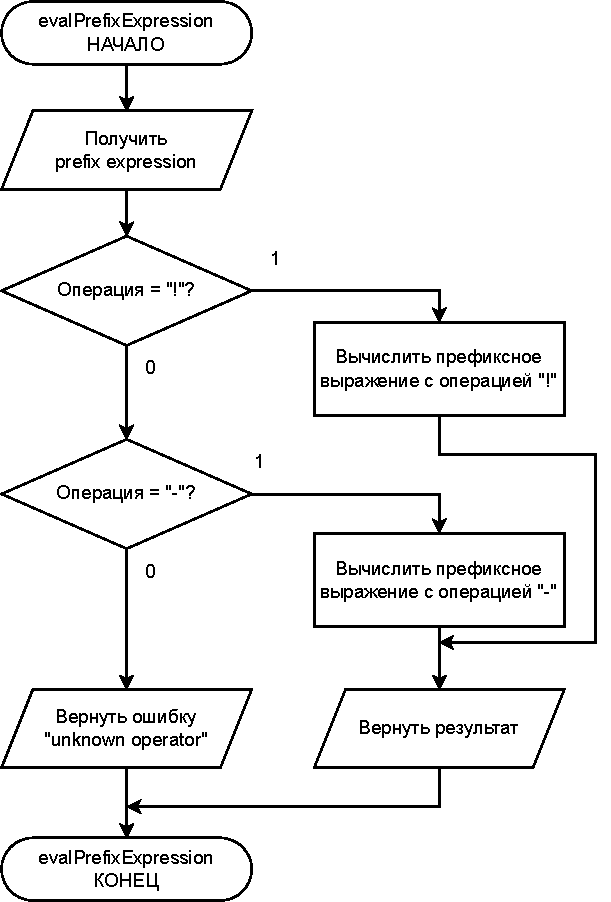
\includegraphics[width=0.9\textwidth]{structures/semantic_analyzer/semantic_prefix_expr.pdf}
	\caption{Схема алгоритма «evalPrefixExpression»}
	\label{f:semantic_prefix_expr}
\end{figure}

\clearpage

\begin{figure}[!htp]
	\centering
	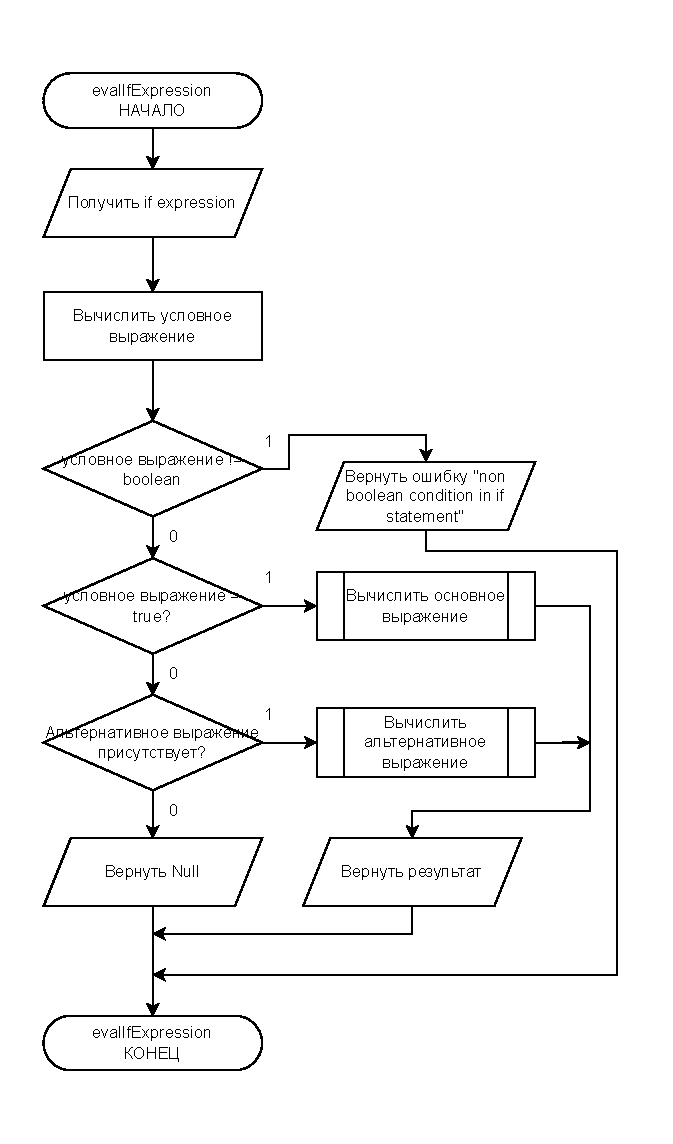
\includegraphics[width=0.7\textwidth]{structures/semantic_analyzer/semantic_if_expr.pdf}
	\caption{Схема алгоритма «evalIfExpression»}
	\label{f:semantic_if_expr}
\end{figure}

\clearpage

\begin{figure}[!htp]
	\centering
	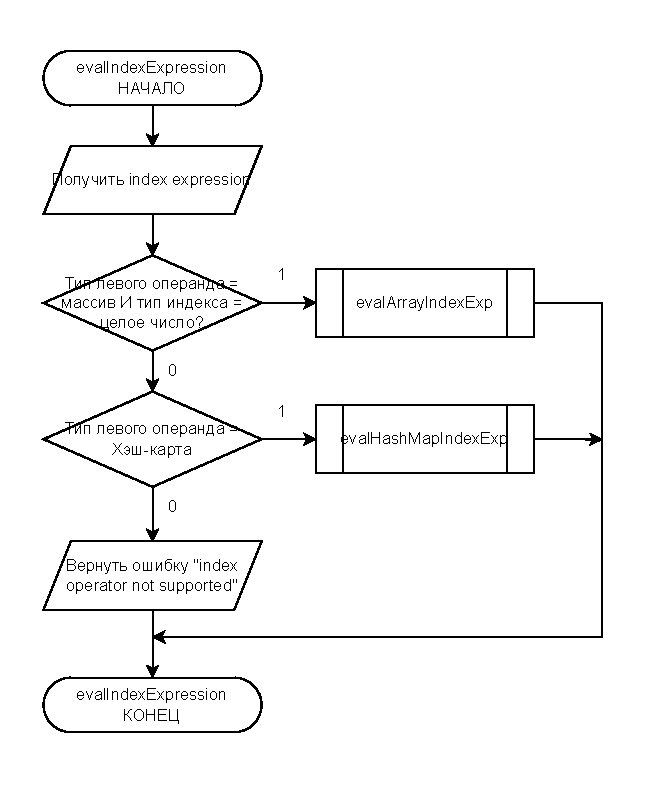
\includegraphics[width=0.75\textwidth]{structures/semantic_analyzer/semantic_index_expr.pdf}
	\caption{Схема алгоритма «evalIndexExpression»}
	\label{f:semantic_index_expr}
\end{figure}
\newpage

\section{Программная реализация}

В данном разделе представлено описание выбранных инструментов разработки для решения поставленной задачи. 
Описана программная реализация модуля интерпретации предметно-ориентированного языка.
Рассмотрены детали реализации его основных структурных частей.
Также выполнено тестирование основных функций программы.

\subsection{Выбор инструментов разработки}

В качестве языка программирования для разработки был выбран Go.

Go (Golang) -- это компилируемый многопоточный язык программирования с открытым исходным кодом, разработанный компанией Google \refref{ref:golang}.

Выбор данного языка обусловлен совместимостью между разрабатываемым модулем и основной системой,
так как для реализации серверной части конструктора Telegram ботов так же был выбран язык Go.
Использование одного языка для всей системы гарантирует,
что модули будут легко интегрироваться друг с другом без необходимости создания сложных интерфейсов или адаптеров.

Язык Go имеет и другие положительные характеристики:
\begin{itemize}
    \item высокая производительность -- Go компилируется в машинный код, что обеспечивает его высокую скорость исполнения;
    \item безопасность типов -- строгая статическая типизация предотвращает множество ошибок на этапе компиляции;
    \item встроенная поддержка параллелизма -- в Go реализованы горутины и каналы -- встроенные механизмы для эффективной работы с параллельными задачами;
    \item расширяемость -- язык имеет встроенную систему управления модулями и широкую экосистему общедоступных библиотек.
\end{itemize}

Выбор языка программирования Go для реализации модуля интерпретации предметно-ориентированного языка конструктора Telegram ботов обоснован тем,
что он позволяет поддерживать единообразие кода, использовать его технические преимущества и соответствовать основным требованиям проекта.

\subsection{Реализация лексического анализатора}

Лексический анализатор состоит из следующих основных компонентов:
\begin{itemize}
    \item токены -- определение структуры и типов токенов, представляющих основные элементы языка;
    \item конечный автомат -- принимает на вход поток символов и определяет токены переходя между состояниями в соответствии с правилами языка.
\end{itemize}

Токен представляет собой структуру, содержащую информацию о типе токена и его значение, представленное в виде строки.
Код структуры, представляющей токен приведен на рисунке~\ref{f:code_tokenStruct}.

\begin{figure}[ht]
	\centering
	\vspace{\toppaddingoffigure}
	\begin{lstlisting}[
        language=Go
    ]
type TokenType = string
type Token struct {
    Type    TokenType
    Literal string
}        
\end{lstlisting}
	\caption{Структура, представляющая токен}
	\label{f:code_tokenStruct}
\end{figure}

Список возможных токенов рассмотрен ранее, см. таблицу~\ref{t:tokens}.

Программную реализацию токенов можно выполнить с помощью списка константных значений.
Фрагмент кода реализации токенов представлен на рисунке~\ref{f:code_tokensFragemnt}.

\begin{figure}[ht]
	\centering
	\begin{lstlisting}
IDENT  = "IDENT"  // x, t, add
INT    = "INT"    // 123
STRING = "STRING" // "abcde"
ASSIGN = "="
PLUS   = "+"
STAR   = "*"
LT  = "<"
GT  = ">"
LAND = "&&"
LOR  = "||"

// keywords
IF     = "IF"
ELSE   = "ELSE"
TRUE   = "TRUE"    
\end{lstlisting}
	\caption{Фрагмент кода реализации токенов}
	\label{f:code_tokensFragemnt}
\end{figure}

Лексер представляет собой структуру, содержащую информацию о входной строке кода,
текущем считанном символе, позиции курсора и других технических значениях, необходимых для корректной работы анализатора.
Структура представляющая лексер приведена на рисунке~\ref{f:code_lexerStruct}.

\begin{figure}[ht]
	\centering
	\vspace{\toppaddingoffigure}
	\begin{lstlisting}[
        language=Go,
        xleftmargin=.08\textwidth,
        xrightmargin=.08\textwidth
    ]
type Lexer struct {
    input   string
    ch      byte // current char
    pos     int  // current position (on current char)
    readPos int  // position after current char
    nlsemi  bool // if "true" '\n' translate to ';'
    loPos   token.Pos
}    
\end{lstlisting}
	\caption{Структура, представляющая лексер}
	\label{f:code_lexerStruct}
\end{figure}

Основная функция лексического анализатора может быть реализована в формате конечного автомата.
При получении очередного символа из входной строки кода его необходимо сопоставить с одним из токенов.
Стоит заметить, что некоторые токены формируются за счет двух и более символом, например токен <<LAND>> (\&\&), идентификаторы, ключевые слова и т.д. 
В этом случае, необходимо продолжать получение символов из входной строки до тех пор, пока не будет однозначно определен токен.

Основная функция определения токена выполнена в виде конструкции switch-case.
Фрагмент кода представлен на рисунке~\ref{f:code_lexerFragment}.

\clearpage

\begin{figure}[!ht]
	\centering
    \begin{lstlisting}[
        language=Go,
        xleftmargin=.08\textwidth,
        xrightmargin=.08\textwidth
    ]
func (l *Lexer) NextToken() (token.Token, token.Pos) {
    l.skipWhitespace()
    nlsemi := false
    var tok token.Token
    switch l.ch {
    case '\n':
        tok = newToken(token.SEMICOLON, l.ch)
    case '=':
        if l.peekChar() == '=' {
            l.readChar()
            literal := "=="
            tok = token.Token{Type: token.EQ, Literal: literal}
        } else {
            tok = newToken(token.ASSIGN, l.ch)
        }
    case '+':
        tok = newToken(token.PLUS, l.ch)
    case '-':
        tok = newToken(token.MINUS, l.ch)
    case '*':
        tok = newToken(token.STAR, l.ch)
    case '/':
        tok = newToken(token.SLASH, l.ch)
    case '!':
        if l.peekChar() == '=' {
            l.readChar()
            literal := "!="
            tok = token.Token{Type: token.NEQ, Literal: literal}
        } else {
            tok = newToken(token.EXCLAMINATION, l.ch)
        }
    case '%':
		tok = newToken(token.PERCENT, l.ch)
	case '<':
		if l.peekChar() == '=' {
			l.readChar()
			literal := "<="
			tok = token.Token{Type: token.LEQ, Literal: literal}
		} else {
			tok = newToken(token.LT, l.ch)
		}
\end{lstlisting}
	\caption{Фрагмент кода лексера}
	\label{f:code_lexerFragment}
\end{figure}
\subsection{Разработка синтаксического анализатора}

% В данном разделе необходимо выполнить разработку алгоритмов функционирования синтаксического анализатора.

Синтаксический анализ – процесс сопоставления последовательности токенов с формальной грамматикой языка.
Результатом работы синтаксического анализатора является абстрактное синтаксическое дерево (AST),
которое отражает синтаксическую структуру входной последовательности и содержит всю необходимую информацию для дальнейших этапов работы транслятора.

В задачу синтаксического анализа входит поиск и выделение основных синтаксических конструкций текста входной программы,
установление типа и проверка правильности каждой синтаксической конструкции, а так же представление их в виде AST.

Существует два основных метода синтаксического анализа:

\begin{itemize}
    \item нисходящий;
    \item восходящий.
\end{itemize}

В данном проекте реализован нисходящий анализатор, работающий по методу рекурсивного спуска,
известный как парсер Пратта, который впервые описал Вон Пратт в статье «Нисходящий парсер с операторным предшествованием».

Этот метод основан на идее приоритета операторов и обработке различных уровней приоритета в выражениях.
В парсере Пратта каждый оператор имеет свой уровень приоритета.
Операторы с более высоким приоритетом связываются с операндами сильнее, чем операторы с более низким приоритетом.
Значения приоритетов для каждого оператора разрабатываемого предметно-ориентированного языка показаны в таблице~\ref{t:operator_priority}.

\clearpage

\begin{table}[h!]
    \Large
    \caption{Приоритеты операторов}
    \label{t:operator_priority}
    \centering
    \begin{tabularx}{\textwidth}{|c|X|}
        \hline
        Приоритет & Операторы             \\
        \hline
        0         & Минимальный приоритет \\
        \hline
        1         & =                     \\
        \hline
        2         & | |                   \\
        \hline
        3         & \&\&                  \\
        \hline
        4         & == !=                 \\
        \hline
        5         & < > <= >=             \\
        \hline
        6         & + -                   \\
        \hline
        7         & * / \%                \\
        \hline
        8         & -x or !x              \\
        \hline
        9         & (                     \\
        \hline
        10        & [                     \\
        \hline
    \end{tabularx}
    \vspace{\bottompaddingoftable}
\end{table}

Для примера работы приоритета операторов рассмотрим пример построения AST для арифметического выражения: $3 + 1 * 4 * 6 + 8$.
Диаграмма, показывающая рекурсивные вызовы для формирования выражений к приведенному примеру изображена на рисунке~\ref{f:priorities}.

\begin{figure}[ht]
	\centering
	\vspace{\toppaddingoffigure}
	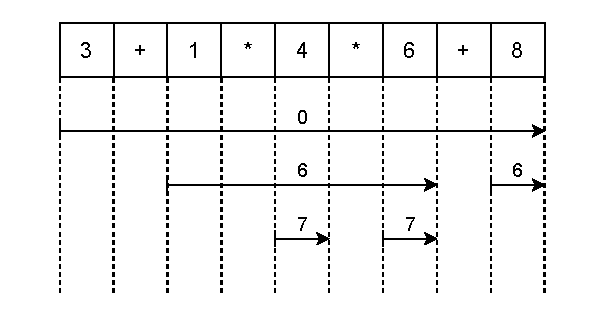
\includegraphics[width=0.7\textwidth]{structures/parser/priorities.pdf}
	\caption{Диаграмма рекурсивных вызовов}
	\label{f:priorities}
\end{figure}

Над стрелками обозначены приоритеты операторов, к которым относится эта стрелка.
В самом начале распознавания выражения значение приоритета равняется 0.
По мере обнаружения оператора, приоритет которого выше текущего алгоритм переходит на следующий уровень рекурсии.
По диаграмме видно, что справа от первого оператора «+» длинная стрелка с приоритетом 6, группирует члены умножения, так как операция умножения имеет больший приоритет, чем сложение.
Эта стрелка заканчивается перед последним «+», так как приоритет оператора, относящегося к этой стрелке не ниже приоритета последнего «+».
Другими словами, экземпляр выражения с более низким приоритетом ожидает результата формирования выражения с более высоким приоритетом.

Абстрактное синтаксическое дерево для данного примера приведено на рисунке~\ref{f:ast_example}.

\begin{figure}[ht]
	\centering
	\vspace{\toppaddingoffigure}
	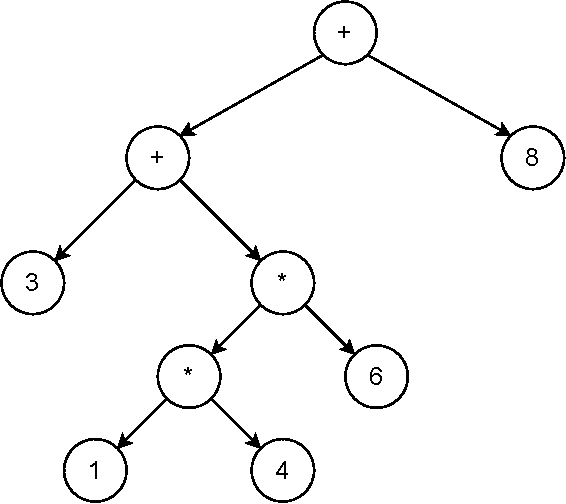
\includegraphics[width=0.7\textwidth]{structures/parser/ast_example.pdf}
	\caption{Абстрактное синтаксическое дерево}
	\label{f:ast_example}
\end{figure}

Некоторые схемы алгоритма построения абстрактного синтаксического дерева представлены на рисунках~\ref{f:parse_program}~-~\ref{f:parse_Expression}.

% В данном разделе была выполнена разработка структурных решений и алгоритмов функционирования синтаксического анализатора.

\clearpage

\begin{figure}[!htp]
	\centering
	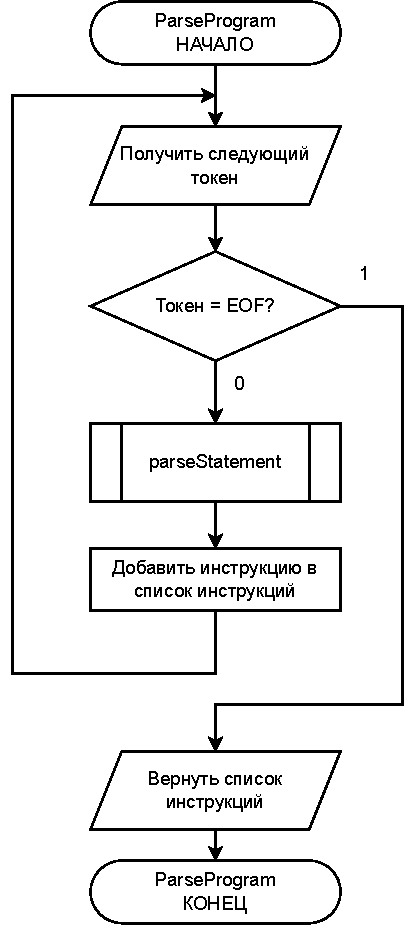
\includegraphics[width=0.5\textwidth]{structures/parser/parse_program.pdf}
	\caption{Схема алгоритма «ParseProgram»}
	\label{f:parse_program}
\end{figure}

\clearpage

\begin{figure}[!htp]
	\centering
	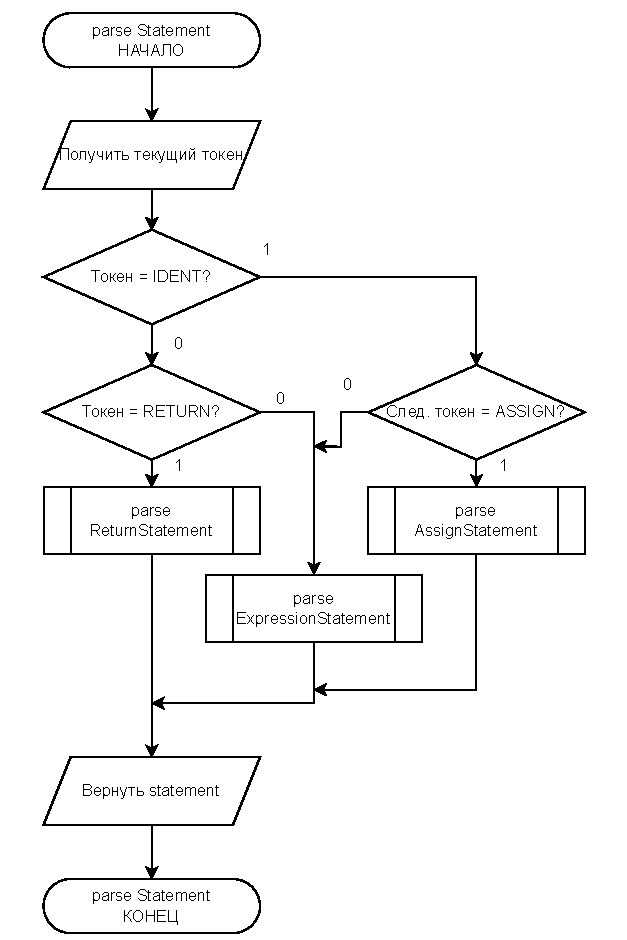
\includegraphics[width=0.7\textwidth]{structures/parser/parse_statement.pdf}
	\caption{Схема алгоритма «parseStatement»}
	\label{f:parse_statement}
\end{figure}

\clearpage

\begin{figure}[!htp]
	\centering
	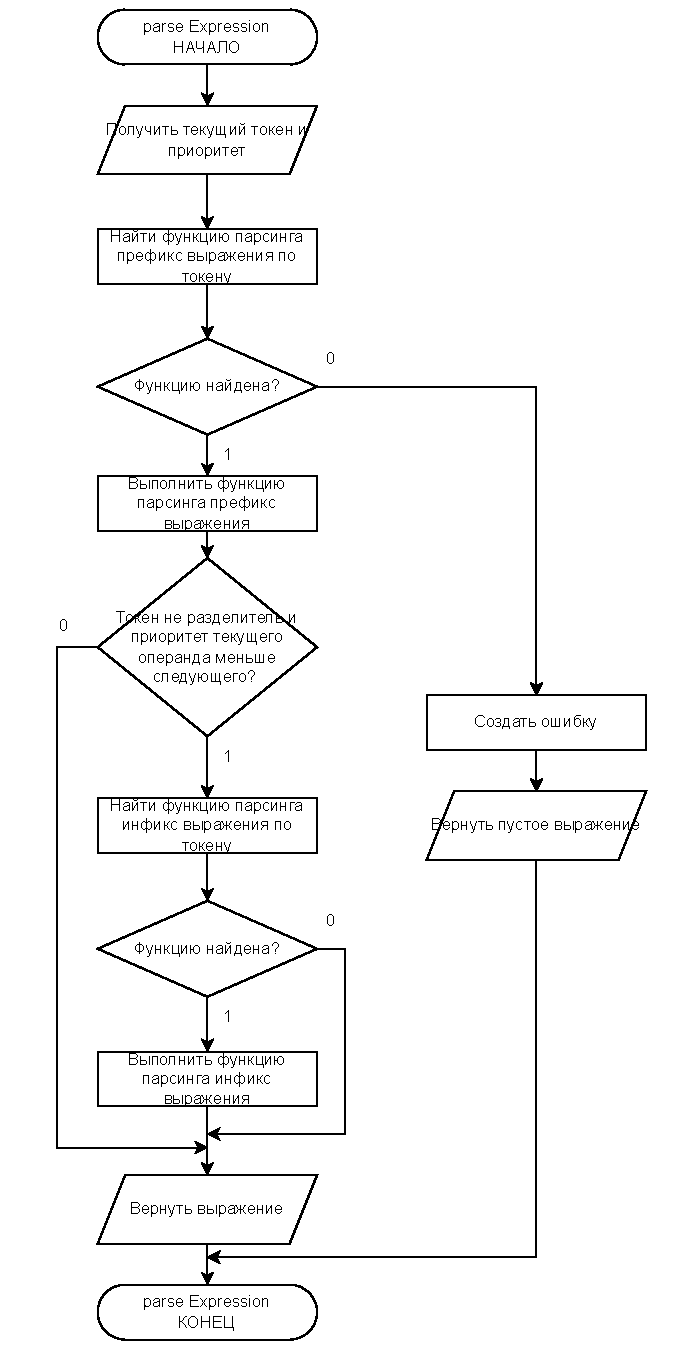
\includegraphics[width=0.60\textwidth]{structures/parser/parse_Expression.pdf}
	\caption{Схема алгоритма «parseExpression»}
	\label{f:parse_Expression}
\end{figure}

\clearpage


\subsection{Разработка семантического анализатора}

% В данном разделе необходимо выполнить разработку алгоритмов функционирования семантического анализатора.

Семантический анализ – это этап работы транслятора, вот время которого выполняется проверка текста исходной программы с точки зрения семантики языка.
В ходе семантического анализа выполняется такие операции, как проверка типов данных, правильность использования переменных, функций, выражений, а также обнаружение смысловых ошибок в коде.

Обобщенная модульная структура серверной части конструктора представлена на рисунке~\ref{f:modules_server_struct}.

Процесс семантического анализа выполняется после построения абстрактного синтаксического дерева синтаксическим анализатором.
Семантический анализ сгруппирован с этапом исполнения выражений.
Таким образом при одном проходе AST алгоритм выполняет проверку узла дерева на семантическую корректность и переход к его исполнению,
если не было обнаружено ошибок при семантическим анализе. В случае обнаружения семантической ошибки возвращается информация о ней,
а процесс интерпретации переход к следующему выражению.

На этапе проектирования семантического анализатора закладываются решения, которые лягут в основу принципов написания кода на разрабатываемом языке.
Например, на этапе построения семантического анализатора, нужно решить, как будет обрабатываться значение в условном выражении, не имеющее тип boolean.
Есть несколько вариантов обработки таких значений.
Один из них - всегда принимать данное значение за «false» и идти в соответствующую ветвь.
В ином случае, при обнаружении значения с типом, отличным от boolean необходимо вернуть ошибку и прекратить выполнение данного выражения.
В этом проекте будет использован второй вариант с возвратом ошибки.

Семантический анализатор принимает на вход элементы абстрактного синтаксического дерева.
После проверки семантической корректности выражения AST, следует его вычисление.
Результаты вычислений выражений, как промежуточные, так и окончательные необходимо каким-то образом представить в памяти.
Это необходимо в первую очередь для получения ранее вычисленных выражений и работы с ними.
В качестве примера можно рассмотреть код, представленный на рисунке~\ref{f:code_example_var}.

\begin{figure}[ht]
	\centering
	\vspace{\toppaddingoffigure}
	\begin{lstlisting}
X = 5;
X + 3
\end{lstlisting}
	\caption{Пример кода использования объявленной переменной}
	\label{f:code_example_var}
\end{figure}

В первой строке присваивается значение 5 переменной «X».
Затем выполняется выражение «X + 3».
Чтобы получить значение данного выражения нужно получить ранее вычисленное значение 5.
Для этого необходимо как-то сохранить его в памяти.

Решение данной задачи состоит в введении внутреннего представления вычисленных значений на время семантического анализа и этапа исполнения.
Примем некоторую объектную систему, состоящую из набора объектов, каждый из которых будет содержать информацию о представляемом им типе данных в предметно-ориентированном языке.

Каждый объект должен содержать информацию о значении представляемого им типа данных предметно-ориентированного языка.
Кроме этого, необходимо реализовать возможность определения того, какой тип данных предметно-ориентированного языка представляет объект, а также функционал получения строкового значения объекта.
Кроме этого, типы данных: целое число, строка и булево значение могут использоваться в виде ключей в хэш-карте.
Для этого необходимо специально для объектов, представляющих эти типы предусмотреть функцию вычисления хэш строки от их значения. 

Объектная система должна представлять все типы данных предметно-ориентированного языка, а именно:
целые числа, строки, булевы значения, массивы, хэш-карты.
Также необходимо ввести дополнительные объекты, представляющие семантические ошибки, значение «null», функции, операцию возврата значения из функции.

Объектная система может быть представлена в виде диаграммы классов.
Диаграмма классов представлена на рисунке~\ref{f:class_diagram}.

\clearpage

\begin{figure}[!htp]
	\centering
    \vspace{\toppaddingoffigure}
	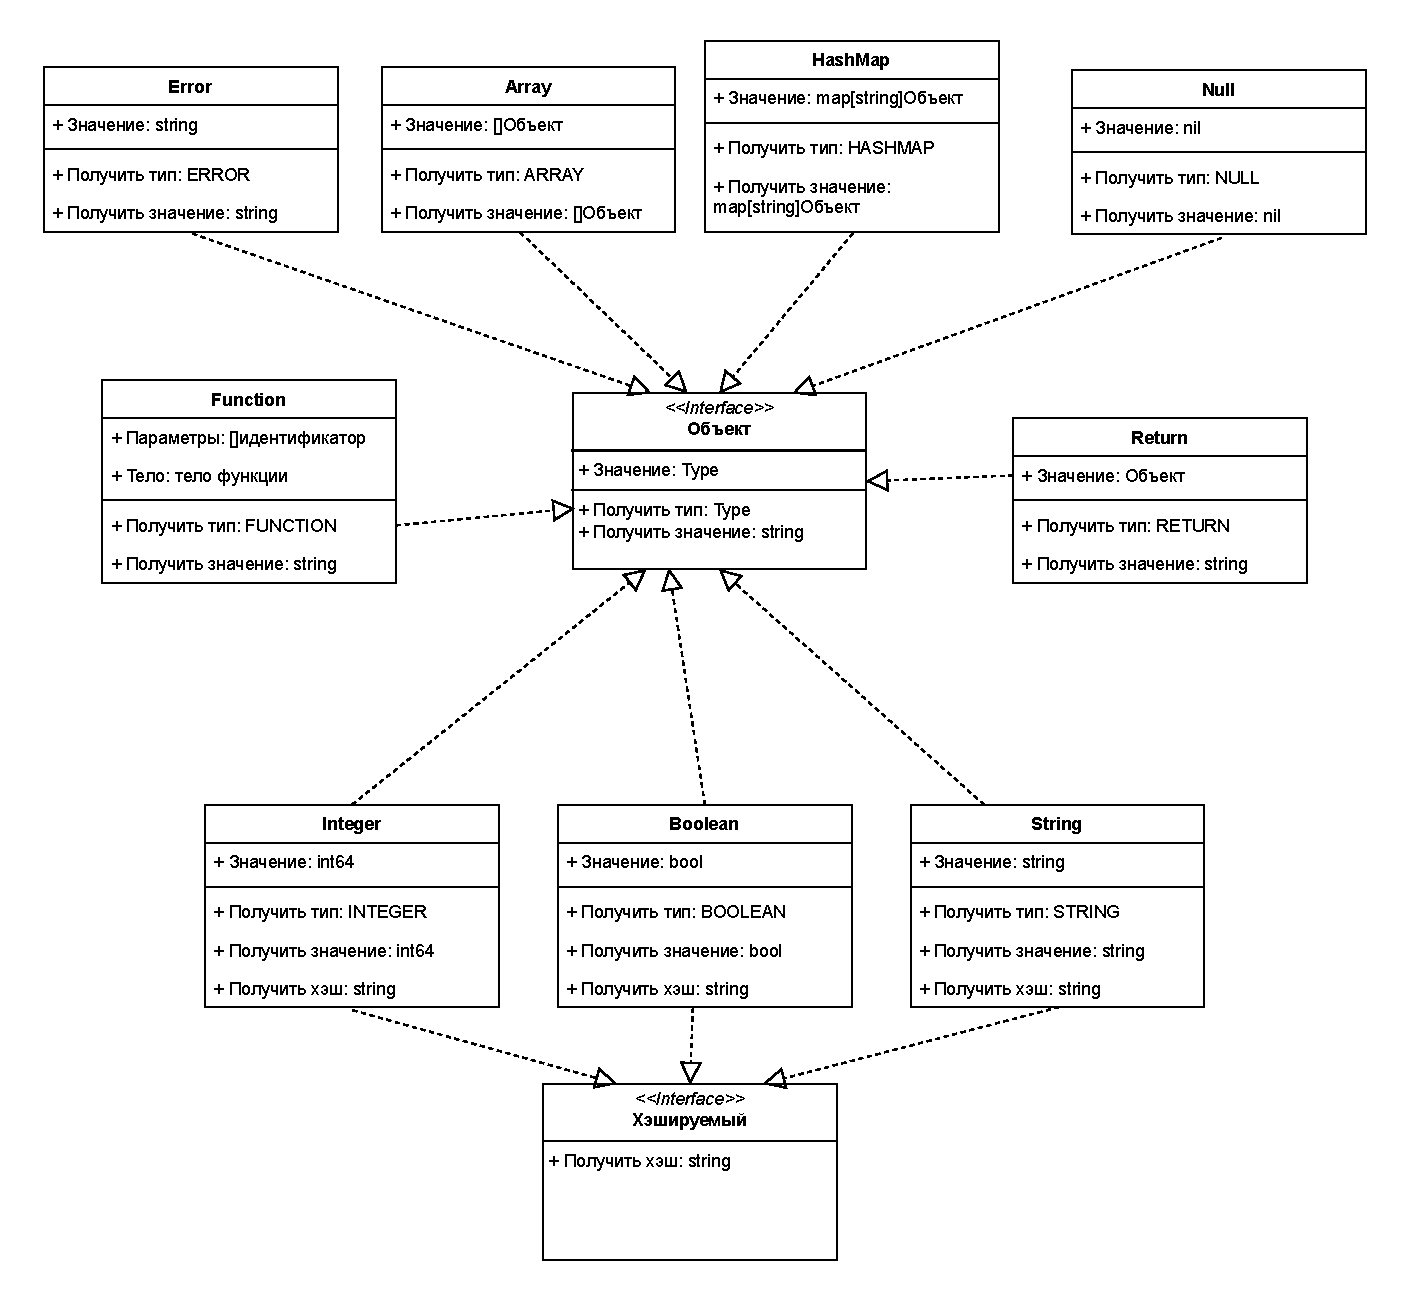
\includegraphics[width=1.0\textwidth]{structures/semantic_analyzer/class_diagram.pdf}
	\caption{Диаграмма классов}
	\label{f:class_diagram}
\end{figure}

В качестве примера работы алгоритма на рисунках~\ref{f:evalProgram}~-~\ref{f:semantic_index_expr} приведены схемы алгоритмов семантического анализа некоторых выражений.

% В данном разделе была выполнена разработка структурных решений и алгоритмов функционирования семантического анализатора.

\begin{figure}[!htp]
	\centering
	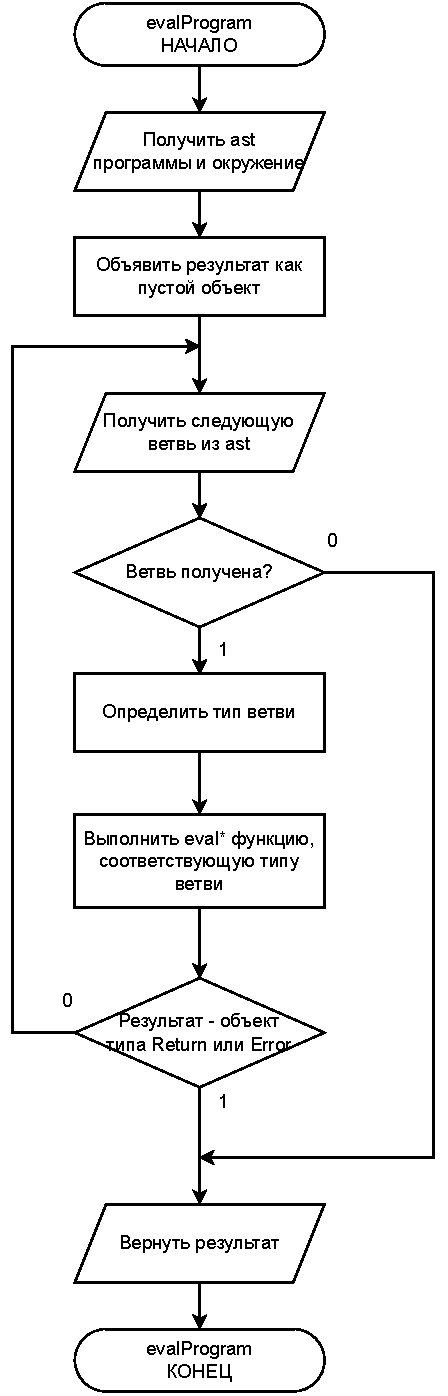
\includegraphics[width=0.4\textwidth]{structures/semantic_analyzer/semantic_Program.pdf}
	\caption{Схема алгоритма «evalProgram»}
	\label{f:evalProgram}
\end{figure}

\clearpage

\begin{figure}[!htp]
	\centering
	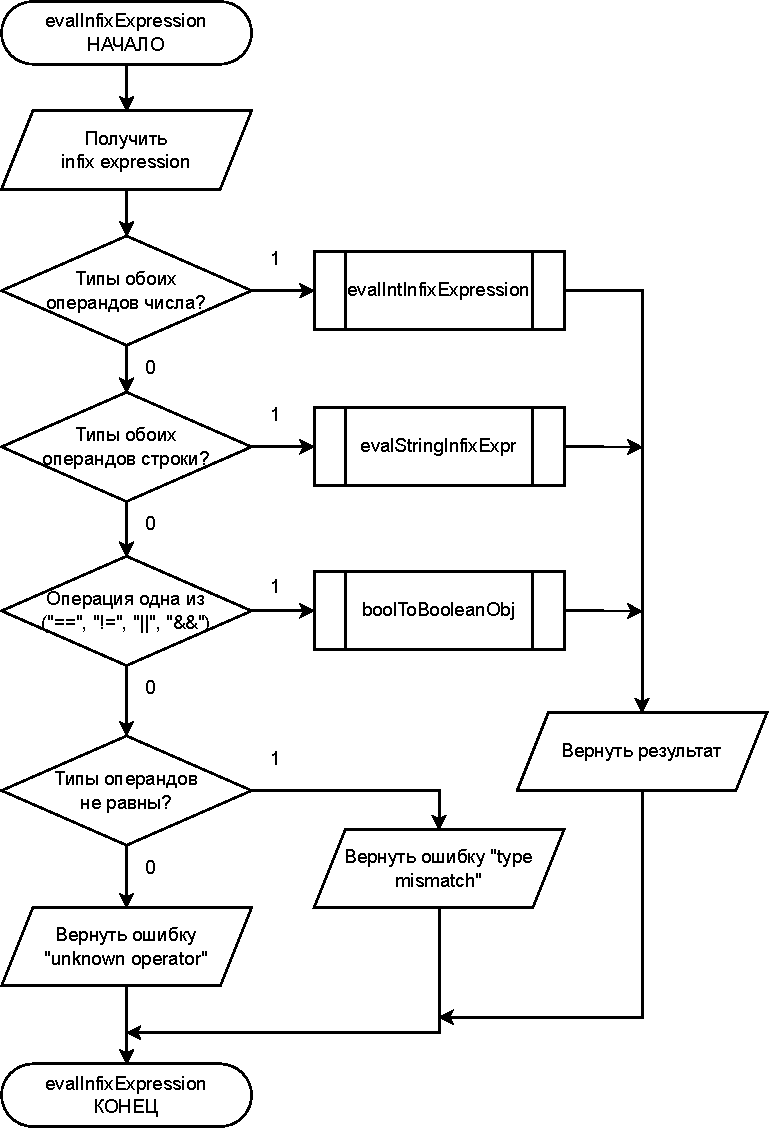
\includegraphics[width=0.9\textwidth]{structures/semantic_analyzer/semantic_infix_expr.pdf}
	\caption{Схема алгоритма «evalInfixExpression»}
	\label{f:semantic_infix_expr}
\end{figure}

\clearpage

\begin{figure}[!htp]
	\centering
	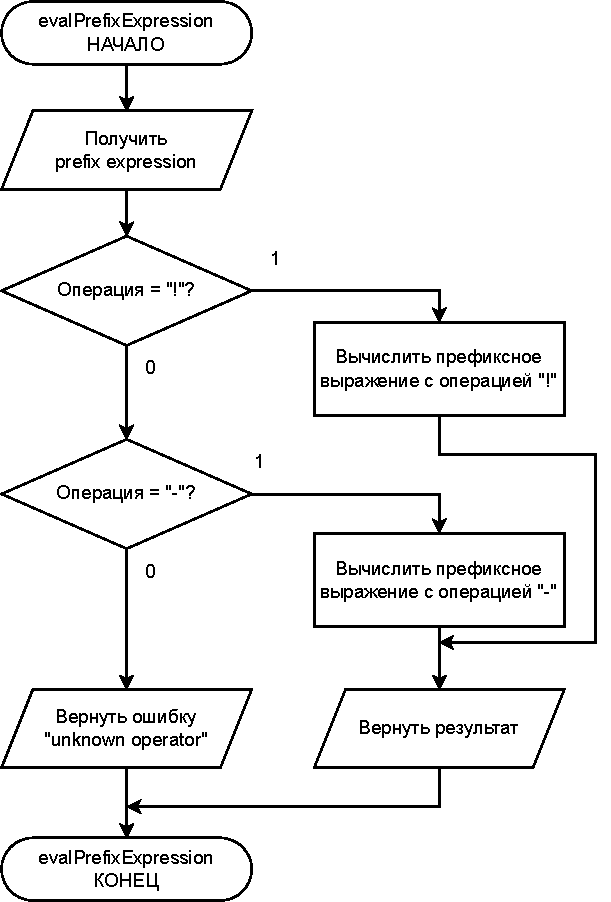
\includegraphics[width=0.9\textwidth]{structures/semantic_analyzer/semantic_prefix_expr.pdf}
	\caption{Схема алгоритма «evalPrefixExpression»}
	\label{f:semantic_prefix_expr}
\end{figure}

\clearpage

\begin{figure}[!htp]
	\centering
	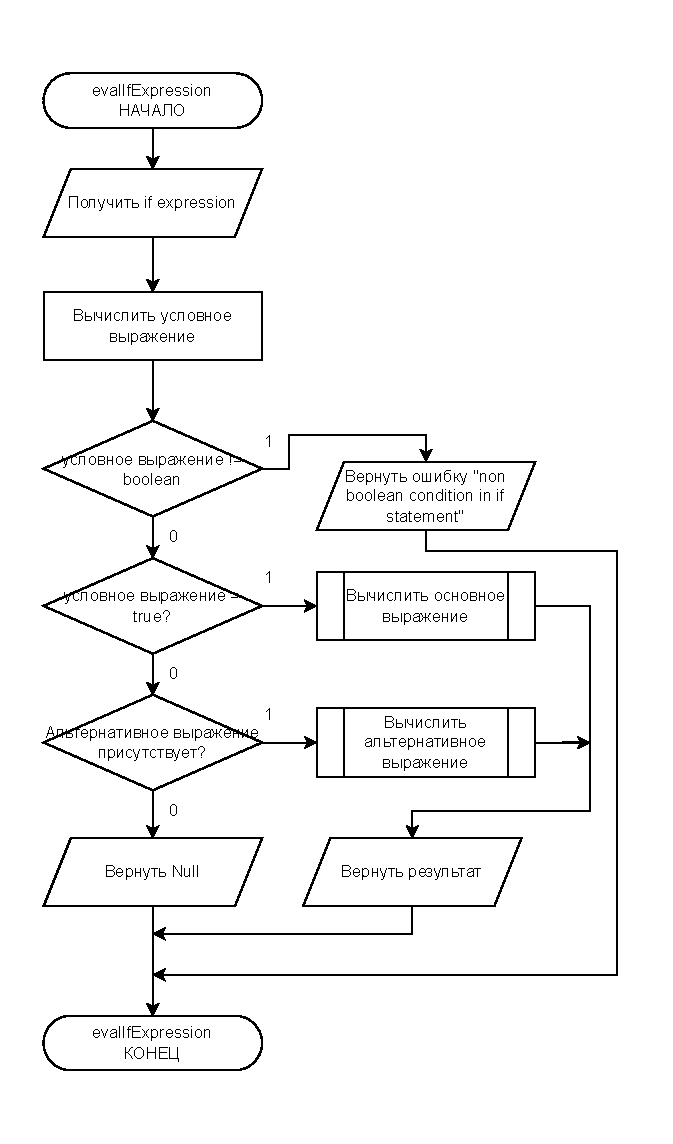
\includegraphics[width=0.7\textwidth]{structures/semantic_analyzer/semantic_if_expr.pdf}
	\caption{Схема алгоритма «evalIfExpression»}
	\label{f:semantic_if_expr}
\end{figure}

\clearpage

\begin{figure}[!htp]
	\centering
	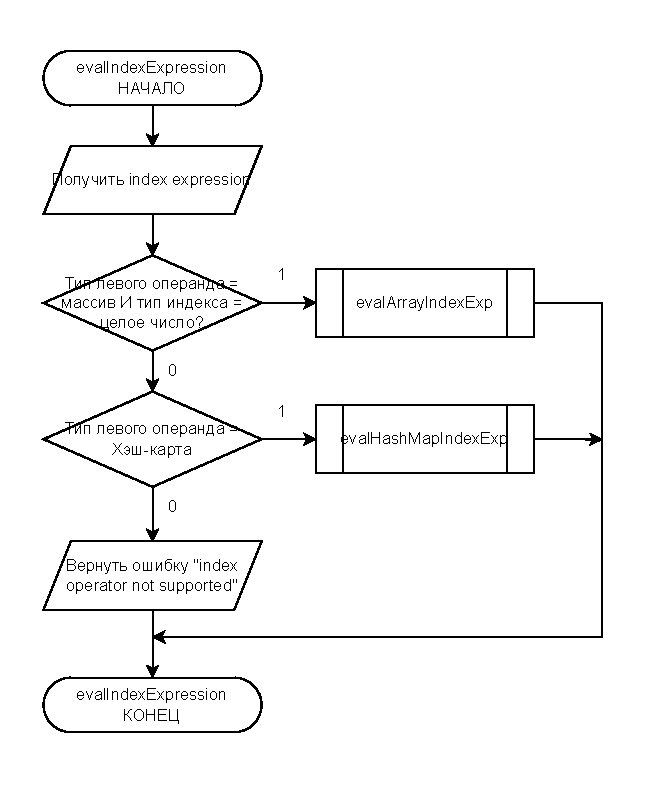
\includegraphics[width=0.75\textwidth]{structures/semantic_analyzer/semantic_index_expr.pdf}
	\caption{Схема алгоритма «evalIndexExpression»}
	\label{f:semantic_index_expr}
\end{figure}
\subsection{Разработка исполнителя}

Процесс вычисления выполняется над выражениями из узлов абстрактного синтаксического дерева.
Такой вид интерпретатора, который работает с AST называется <<tree walking interpreter>> или древовидный интерпретатор.
В таком интерпретаторе выполняется обход AST и выполнение соответствующих операций для каждого узла.

Последним этапом в процессе обработки исходного кода является его исполнение.
До этого шага все выражения языка представляют собой набор символов, токенов или ветви абстрактного синтаксического дерева без какого-либо семантического значения.
На данном этапе выражения языка приобретают смысл, то есть начинают интерпретироваться и действовать в соответствии с правилами и инструкциями языка.

Этап исполнения выполняется непосредственно после семантического анализа.
Если во время семантического анализа в обрабатываемом выражении не было обнаружено ошибок, выполняется переход к его вычислению.
Вычисление выражения выполняется в зависимости от его типа, например,
для инфиксного выражения применяется указанная в нем операция над левым и правым операндами и формируется результат в виде объекта соответствующего типа,
содержащего результат операции, а для условного выражения сначала вычисляется значение условия,
а затем в зависимости от его результата выполняется либо основная ветвь (при значении условия «true»), либо альтернативная (при значении условия «false»).

Только лишь вычислять значения выражений недостаточно.
Нужно также сохранять значения переменных для того, чтоб к ним можно было обратиться при обнаружении в выражениях.
Чтобы обеспечить эту возможность введем окружение – структуру данных, хранящую информацию о переменных и связанных с ними значениях на время выполнения программы.
Таким образом, при объявлении переменной, информация о ней будет записываться в окружение, а при необходимости получить значение этой переменой – ее значение будет считано из окружения.

В качестве примера работы алгоритма на рисунках~\ref{f:eval_int_infix_expr}~-~\ref{f:eval_string_infix_expr} приведены схемы алгоритма вычисления некоторых выражений.

\clearpage

\begin{figure}[!htp]
	\centering
	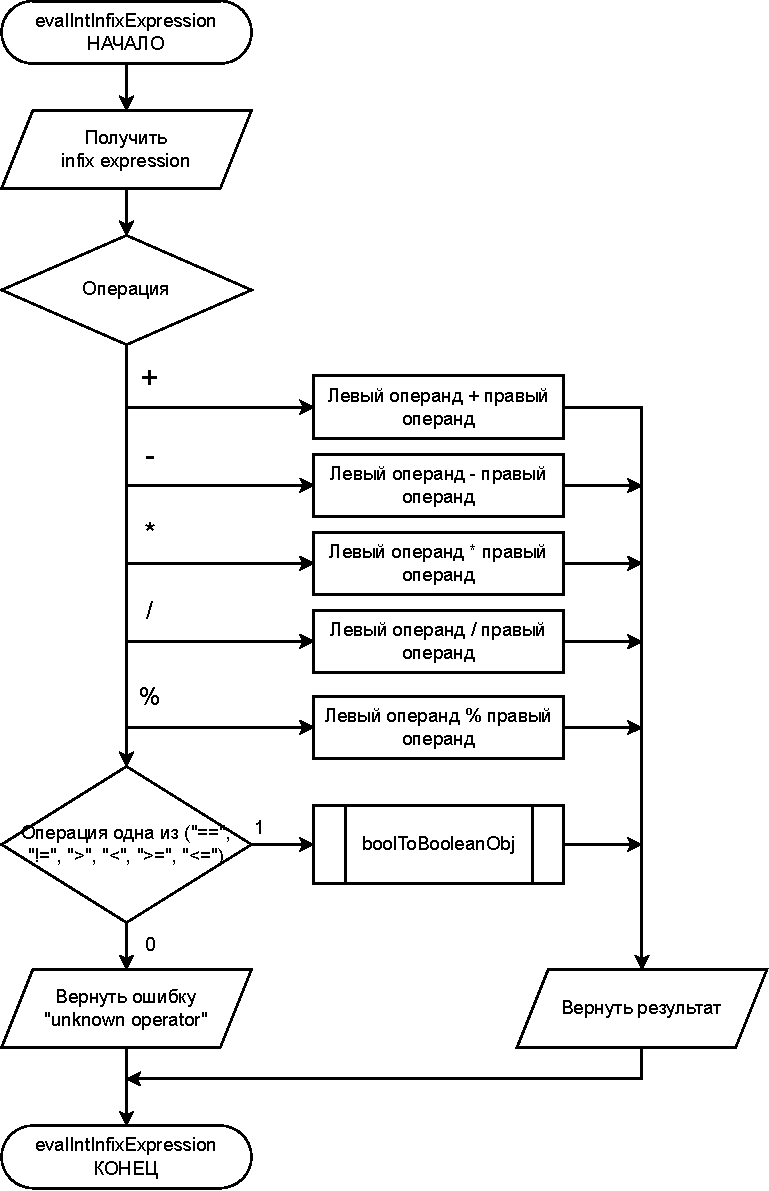
\includegraphics[width=0.8\textwidth]{structures/evaluator/eval_int_infix_expr.pdf}
	\caption{Схема алгоритма вычисления целочисленного инфиксного выражения}
	\label{f:eval_int_infix_expr}
\end{figure}

\clearpage

\begin{figure}[!htp]
	\centering
	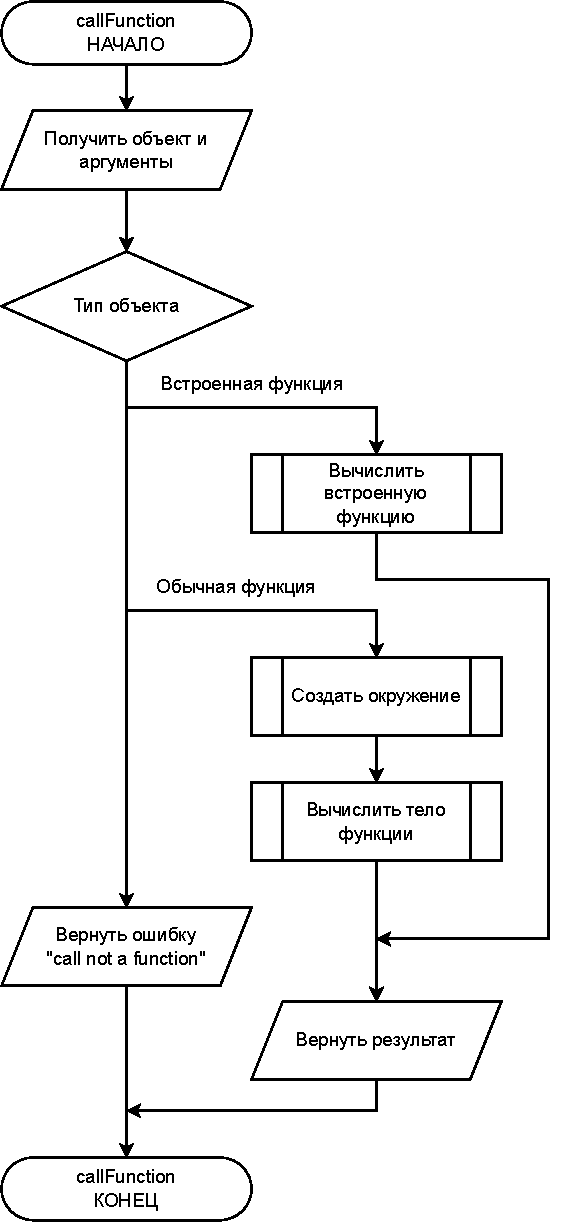
\includegraphics[width=0.6\textwidth]{structures/evaluator/eval_callFunction.pdf}
	\caption{Схема алгоритма исполнения вызова функции}
	\label{f:eval_callFunction}
\end{figure}

\clearpage

\begin{figure}[!htp]
	\centering
	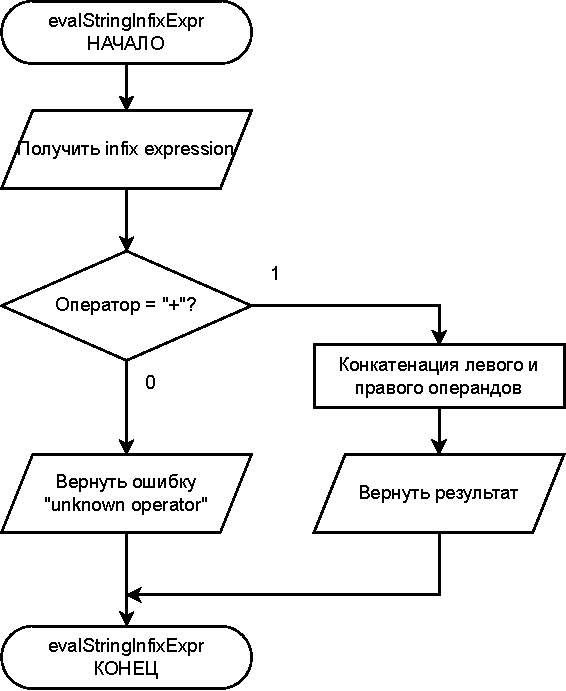
\includegraphics[width=0.5\textwidth]{structures/evaluator/eval_string_infix_expr.pdf}
	\caption{Схема алгоритма вычисления инфиксного выражения для строк}
	\label{f:eval_string_infix_expr}
\end{figure}
\subsection{Тестирование}

Тестирование является одним из ключевых этапов разработки, направленным на подтверждение корректности работы программы.

Выделяют три основных вида тестирования:
\begin{itemize}
    \item модульное тестирование;
    \item интеграционное тестирование;
    \item функциональное тестирование.
\end{itemize}

Модульное тестирование или юнит-тестирование позволяет проверить отдельные изолированные компоненты системы.
Направлено на проверку правильности функционирования каждого блока с помощью входных данных и подтверждения соответствия результата теста ожидаемым результатам.

Интеграционное тестирование направлено на проверку корректности взаимодействия нескольких модулей как единой группы.
Интеграционные тесты позволяют выявить проблемы, связанные с зависимостями и обменом информацией между компонентами системы.

Функциональное тестирование -- ип тестирования, который направлен на проверку соответствия работы программы заданной функциональности.
Основная цель -- убедиться, что разработанное программное обеспечение работает правильно и обеспечивает требуемую функциональность.

Проверка корректности работы лексера, парсера, семантического анализатора и исполнителя выполнена с помощью модульных тестов.
Написаны тесты для большинства основных функций.
Некоторые тест-кейсы приведены в таблицах~\ref{t:testCases_infixIntExpr}-13.

Для реализации и запуска тестов в разработанной программе использовалась встроенная среду выполнения Go утилита go test.
Эта утилита предоставляет удобный и мощный инструмент для создания и выполнения тестов, включая модульные и функциональные тесты.
Go test позволяет одной командой запускать все реализованные тест-кейсы в проекте и получать результат их выполнения.

% Фрагменты кода тестирования представлены в приложении Д.

В ходе запуска тестирования все тесты выполнились успешно. Результат тестирования представлен на рисунке~\ref{f:testResult}.

\begin{figure}[ht]
    \centering
    \vspace{\toppaddingoffigure}
    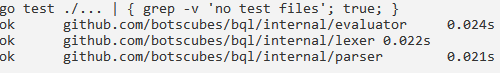
\includegraphics[width=0.9\textwidth]{evaluator/testResult.png}
    \caption{Результаты запуска тестов}
    \label{f:testResult}
\end{figure}

\clearpage

\begin{table}[!ht]
    \Large
    \centering
    \begin{threeparttable}
        \caption{Тест-кейсы исполнения целочисленного выражения}
        \label{t:testCases_infixIntExpr}
        \begin{tabularx}{\textwidth}{|X|c|}
            \hline
            Входные данные                & Ожидаемый результат \\
            \hline
            4                             & 4                   \\
            \hline
            -5                            & -5                  \\
            \hline
            2 + 2                         & 4                   \\
            \hline
            1 + 2 + 3 + 4 + 5 - 1 - 2 - 3 & 9                   \\
            \hline
            2 * 3 * 4 * 5 * 6 * 7 * 8 * 9 & 362880              \\
            \hline
            10 + 10 * 2                   & 30                  \\
            \hline
            (10 + 10) * 2                 & 40                  \\
            \hline
            100 / 2 * 2 + 5               & 105                 \\
            \hline
            100 / (2 * 2) - 200           & -175                \\
            \hline
            5 \% 2                        & 1                   \\
            \hline
            4 \% 2                        & 0                   \\
            \hline
        \end{tabularx}
    \end{threeparttable}
    \vspace{\bottompaddingoftable}
\end{table}

\begin{table}[!ht]
    \Large
    \centering
    \begin{threeparttable}
        \caption{Тест-кейсы исполнения встроенных функций}
        \label{t:testCases_builtins}
        \begin{tabularx}{\textwidth}{|X|c|}
            \hline
            Входные данные            & Ожидаемый результат                        \\
            \hline
            len("abc")                & 3                                          \\
            \hline
            len("abc" + "efg")        & 6                                          \\
            \hline
            len("")                   & 0                                          \\
            \hline
            len(1)                    & type of argument not supported: INTEGER    \\
            \hline
            len("a", "b")             & wrong number of arguments: 2 want: 1       \\
            \hline
            x = "abc"; len(x)         & 3                                          \\
            \hline
            len({[}{]})               & 0                                          \\
            \hline
            x = {[}1, 2, 3{]}; len(x) & 3                                          \\
            \hline
            push({[}{]}, 4)           & {[}4{]}                                    \\
            \hline
            push({[}1, 2, 3{]}, 4)    & {[}1, 2, 3, 4{]}                           \\
            \hline
            push("a", 4)              & first argument must be ARRAY, got: STRING" \\
            \hline
            first({[}{]})             & null                                       \\
            \hline
            first({[}1{]})            & 1                                          \\
            \hline
            first({[}3, 2, 1{]})      & 3                                          \\
            \hline
            first("a")                & argument must be ARRAY, got: STRING        \\
            \hline
            last({[}{]})              & null                                       \\
            \hline
            last({[}1{]})             & 1                                          \\
            \hline
        \end{tabularx}
    \end{threeparttable}
    \vspace{\bottompaddingoftable}
\end{table}

\clearpage

\begin{table}[!ht]
    \Large
    \centering
    \begin{threeparttable}
        \caption{Тест-кейсы семантических ошибок}
        \label{t:testCases_semanticErrors}
        \begin{tabularx}{\textwidth}{|X|c|}
            \hline
            Входные данные                   & Ожидаемый результат                   \\
            \hline
            true + false                     & unknown operator: BOOLEAN + BOOLEAN   \\
            \hline
            1; true - false; 2               & unknown operator: BOOLEAN - BOOLEAN   \\
            \hline
            1; true + false + true + true; 2 & unknown operator: BOOLEAN + BOOLEAN   \\
            \hline
            -true                            & unknown operator: -BOOLEAN            \\
            \hline
            true + 3                         & type mismatch: BOOLEAN + INTEGER      \\
            \hline
            3 * false                        & type mismatch: INTEGER * BOOLEAN      \\
            \hline
            "Hello" * 3                      & type mismatch: STRING * INTEGER       \\
            \hline
            "Hello" * "Earth"                & unknown operator: STRING * STRING     \\
            \hline
            if (3) \{ 1 \}                   & non boolean condition in if statement \\
            \hline
            x = 10; q                        & identifier not found: q               \\
            \hline
            true{[}1{]}                      & index operator not supported: BOOLEAN \\
            \hline
            123{[}123{]}                     & index operator not supported: INTEGER \\
            \hline
        \end{tabularx}
    \end{threeparttable}
    \vspace{\bottompaddingoftable}
\end{table}

\begin{table}[!ht]
    \Large
    \centering
    \begin{threeparttable}
        \caption{Тест-кейсы исполнения вызова функции}
        \label{t:testCases_fnCall}
        \begin{tabularx}{\textwidth}{|X|c|}
            \hline
            Входные данные                                              & Ожидаемый результат \\
            \hline
            x = fn(x)\{ x \}; x(10);                                    & 10                  \\
            \hline
            x = fn(x, y)\{ return x * y \}; x(10, 9);                   & 90                  \\
            \hline
            x = fn(x, y, z)\{ return x * (y - z) \}; x(10,   9, 1);     & 80                  \\
            \hline
            x = fn(x, y)\{ return x + y \}; x(10, x(x(1, 1), x(3, 5))); & 20                  \\
            \hline
            fn(x)\{ x \}(5)                                             & 5                   \\
            \hline
            c = fn(x)\{                                                 & 9                   \\
            fn(y) \{ x + y \}                                           &                     \\
            \}                                                          &                     \\
            a = c(5);                                                   &                     \\
            a(4)                                                        &                     \\
            \hline
        \end{tabularx}
    \end{threeparttable}
    \vspace{\bottompaddingoftable}
\end{table}


\begin{table}[!ht]
    \Large
    \centering
    \begin{threeparttable}
        \caption{Тест-кейсы исполнения массива}
        \label{t:testCases_arrayExprt}
        \begin{tabularx}{\textwidth}{|X|c|}
            \hline
            Входные данные          & Ожидаемый результат \\
            \hline
            {[}1, 2, -33, 5+5, 1 + 2 + 3 + 4 * 5{]}          & {[}1, 2, -33, 10, 26{]}         \\
            \hline
        \end{tabularx}
    \end{threeparttable}
    \vspace{\bottompaddingoftable}
\end{table}

\clearpage

\begin{table}[!ht]
    \Large
    \centering
    \begin{threeparttable}
        \caption{Тест-кейсы исполнения строкового выражения}
        \label{t:testCases_stringExpr}
        \begin{tabularx}{\textwidth}{|X|c|}
            \hline
            Входные данные          & Ожидаемый результат \\
            \hline
            "Hello Earth"           & Hello Earth         \\
            \hline
            "Hello" + " " + "Earth" & Hello Earth         \\
            \hline
        \end{tabularx}
    \end{threeparttable}
    \vspace{\bottompaddingoftable}
\end{table}

\begin{table}[!ht]
    \Large
    \centering
    \begin{threeparttable}
        \caption{Тест-кейсы исполнения булева выражения}
        \label{t:testCases_boolExpr}
        \begin{tabularx}{\textwidth}{|X|c|}
            \hline
            Входные данные              & Ожидаемый результат \\
            \hline
            true                        & true                \\
            \hline
            false                       & false               \\
            \hline
            1 == 1                      & true                \\
            \hline
            1 != 1                      & false               \\
            \hline
            1 \textless 2               & true                \\
            \hline
            1 \textgreater 2            & false               \\
            \hline
            1 \textless{}= 2            & true                \\
            \hline
            1 \textless{}= 1            & true                \\
            \hline
            1 \textgreater{}= 2         & false               \\
            \hline
            1 \textgreater{}= 1         & true                \\
            \hline
            true == true                & true                \\
            \hline
            false == false              & true                \\
            \hline
            true == false               & false               \\
            \hline
            true != false               & true                \\
            \hline
            (true == false) == false    & true                \\
            \hline
            (1 == 1) == true            & true                \\
            \hline
            (1 \textless{}= 1) == false & false               \\
            \hline
            true || false               & true                \\
            \hline
            true \&\& false             & false               \\
            \hline
            true \&\& true              & true                \\
            \hline
            false \&\& false            & false               \\
            \hline
            false || false              & false               \\
            \hline
            !true                       & false               \\
            \hline
            !false                      & true                \\
            \hline
            !!false                     & false               \\
            \hline
        \end{tabularx}
    \end{threeparttable}
    \vspace{\bottompaddingoftable}
\end{table}

\clearpage

\begin{table}[!ht]
    \Large
    \centering
    \begin{threeparttable}
        \caption{Тест-кейсы исполнения условного выражения}
        \label{t:testCases_conditionExpr}
        \begin{tabularx}{\textwidth}{|X|c|}
            \hline
            Входные данные                                 & Ожидаемый результат \\
            \hline
            if (true) \{ 50 \}                             & 50                  \\
            \hline
            if (false) \{ 50 \}                            & null                \\
            \hline
            if (!false) \{ 50 \}                           & 50                  \\
            \hline
            if (1 \textless 2) \{ 50 \} else \{ 100 \}     & 50                  \\
            \hline
            if (1 \textgreater 2) \{ 50 \} else \{ 100 \}  & 100                 \\
            \hline
            if (true || false) \{ 50 \} else \{ 100 \}     & 50                  \\
            \hline
            if (true   \&\& false) \{ 50 \} else \{ 100 \} & 100                 \\
            \hline
        \end{tabularx}
    \end{threeparttable}
    \vspace{\bottompaddingoftable}
\end{table}

\begin{table}[!ht]
    \Large
    \centering
    \begin{threeparttable}
        \caption{Тест-кейсы исполнения индексного выражения для массива}
        \label{t:testCases_arrayIndexExpr}
        \begin{tabularx}{\textwidth}{|X|c|}
            \hline
            Входные данные                                    & Ожидаемый результат \\
            \hline
            {[}1, 2, 5{]}{[}0{]}                              & 1                   \\
            \hline
            {[}1, 2, 5{]}{[}2{]}                              & 5                   \\
            \hline
            {[}1, 2, 5{]}{[}3{]}                              & null                \\
            \hline
            {[}1, 2, 5{]}{[}-1{]}                             & null                \\
            \hline
            {[}1, 2, 5{]}{[}1+1{]}                            & 5                   \\
            \hline
            x = 1; {[}1, 2, 5{]}{[}x{]}                       & 2                   \\
            \hline
            a = {[}1, 2, 5{]}; a{[}0{]} + a{[}1{]} * a{[}2{]} & 11                  \\
            \hline
        \end{tabularx}
    \end{threeparttable}
    \vspace{\bottompaddingoftable}
\end{table}

\begin{table}[!ht]
    \Large
    \centering
    \begin{threeparttable}
        \caption{Тест-кейсы исполнения индексного выражения для хэш-карты}
        \label{t:testCases_HashMapIndexExpr}
        \begin{tabularx}{\textwidth}{|X|c|}
            \hline
            Входные данные                                    & Ожидаемый результат \\
            \hline
            \{"x": 1\}{[}"x"{]}   & 1    \\
            \hline
            \{"x": 1\}{[}"y"{]}   & null \\
            \hline
            \{\}{[}"y"{]}         & null \\
            \hline
            \{5: 2\}{[}5{]}       & 2    \\
            \hline
            \{true: 5\}{[}true{]} & 5    \\
            \hline
        \end{tabularx}
    \end{threeparttable}
    \vspace{\bottompaddingoftable}
\end{table}

\section*{Вывод}

В данном разделе на основании разработанных архитектурно-структурных решениях и алгоритмах функционирования выполнена программная реализация модуля интерпретации предметно-ориентированного языка.
С помощью выбранных инструментов разработки выполнена программная реализация лексического анализатора, синтаксического анализатора, семантического анализатора и исполнителя.

Также на базе встроенной в среду выполнения Go утилиты <<go test>> были реализованы юнит-тесты, охватывающие большинство функций модуля интерпретации.
\newpage

\csection{Заключение}

В ходе выполнения выпускной квалификационной работы выполнена разработка предметно-ориентированного языка для конструктора Telegram ботов и интерпретатора для него.
Основной целью проекта было расширение функциональных возможностей визуального конструктора Telegram ботов.
Благодаря использованию DSL можно более гибко настроить логику работы бота и предоставить пользователю платформы возможность построения сложных, уникальных ботов,
которых было бы невозможно или затруднительно построить с использованием только базового набора компонентов визуального конструктора.

На основе анализа предметной области и определения основных функциональных возможностей предметно-ориентированного языка было сформировано расширенное технического задание,
определяющее требования к разрабатываемому продукту.

Исходя из требований технического задания первоочередной задачей было разработать и описать грамматику предметно-ориентированного языка.
Для описания формальной грамматики была выбрана расширенная форма Бэкуса-Наура.

Была выполнена разработка архитектурно-структурных решений и алгоритмов функционирования каждой составляющей части модуля интерпретации,
а именно лексического, синтаксического, семантического анализаторов и исполнителя инструкций предметно-ориентированного языка.
Также описан программный интерфейс интеграции модуля с серверной частью конструктора.

На этапе программной реализации были выполнено кодирование анализаторов и исполнителя
в соответствии с разработанными алгоритмами функционирования с помощью выбранных инструментов разработки.
Кроме этого было осуществлено модульное тестирование разработанной программы.

Разработанный предметно-ориентированный язык позволяет расширить функциональные возможности конструктора Telegram ботов.
\docappendix{Листинг кода}

\begin{lstlisting}
var a = 1;
var b = 10;
var c = 123;
var d = a + b + c;

some_function(a, b, c);
\end{lstlisting}


\docappendix{Авторская справка}
\begin{singlespace}

	\newcommand{\authorfullname}{Волков Михаил Владимировч}
	\renewcommand{\authorwithinitials}{Волков М. В.}
	\renewcommand{\headofdepartment}{М. Л. Долженкова}

	Я, \authorfullname , автор выпускной квалификационной
	работы «\topic» сообщаю, что мне известно о персональной ответственности автора
	за разглашение сведений, подлежащих защите законами РФ о защите объектов
	интеллектуальной собственности.

	Одновременно сообщаю, что:

	1. При подготовке к защите выпускной квалификационной работы не
	использованы источники (документы, отчёты, диссертации, литература и т.п.),
	имеющие гриф секретности или «Для служебного пользования» ФГБОУ ВО
	«Вятский государственный университет» или другой организации.

	2. Данная работа не связана с незавершёнными исследованиями или уже
	с завершёнными, но ещё официально не разрешёнными к опубликованию
	ФГБОУ ВО «Вятский государственный университет» или другими
	организациями.

	3. Данная работа не содержит коммерческую информацию, способную
	нанести ущерб интеллектуальной собственности ФГБОУ ВО «Вятский
	государственный университет» или другой организации.

	4. Данная работа не является результатом НИР или ОКР, выполняемой по
	договору с организацией.

	5. В предлагаемом к опубликованию тексте нет данных по
	незащищённым объектам интеллектуальной собственности других авторов.

	6. Использование моей дипломной работы в научных исследованиях
	оформляется в соответствии с законодательством РФ о защите интеллектуальной
	собственности отдельным договором.

	\newcommand{\daysize}{2em}

	\newcommand{\confirm}{
		\noindent
		Сведения по авторской справке подтверждаю:~«\uline{\hspace{\daysize}}»
	}

	\newcommand{\verticalspacesize}{2em}

	\newcommand{\rightindent}{2em}

	\newcommand{\customtheyear}{\the\year~г.}

	\newcommand{\rightindentwithyear}{\widthof{\customtheyear}+\rightindent}

	\newcommand{\signaturesize}{6.6em}

	\vspace{\verticalspacesize}


	\noindent
	Автор: \authorwithinitials~«\uline{\hspace{\daysize}}»
	\uline{\hspace{6em}}
	\customtheyear
	\hfill
	\uline{\hspace{\signaturesize}}\hspace{\rightindentwithyear}

	\vspace{-0.3em}
	\hfill
	\makebox[\signaturesize][c]{\small подпись}
	\hspace{\rightindentwithyear}

	\vspace{\verticalspacesize}

	\confirm
	\uline{\hfill}\customtheyear\hspace{\rightindent}

	\vspace{\verticalspacesize}

	\noindent
	Заведующая кафедрой ЭВМ: \headofdepartment
	\hfill
	\uline{\hspace{\signaturesize}}\hspace{\rightindentwithyear}

	\vspace{-0.3em}
	\hfill
	\makebox[\signaturesize][c]{\small подпись}
	\hspace{\rightindentwithyear}

\end{singlespace}



\docappendix[справочное]{Какое-то справочное приложение}


Содержимое приложения

% \newpage

\csection{Библиографический список}

\begin{references}
	\item\label{ref:num-methods} Бахвалов Н.С., Жидков Н.П., Кобельников Г.М.
	Численные методы [Текст] – 4-е изд. – М:. БИНОМ. Лаборатория
	знаний, 2006. – 636 с.: ил.
	\item Безрученко Б.П., Смирнов Д.А.
	Статистическое моделирование по временным рядам [Электронный ресурс]
	Cарат. отд-ние Ин-та радиотехники и электроники РАН.
	– Электрон. дан. – Саратов, 2000. – Режим доступа:
	http://www.masters.donntu.edu.ua/2012/fknt/dorosh/library/article4.pdf,
	свободный. - Загл. с экрана.
	\item\label{ref:time-series-analysis} Бокс Дж., Дженкинс Г. Анализ временных рядов.
	Прогноз и управление [Текст]. - М.: Мир, 1974.
\end{references}

}{
	% Привер файла содержимого документа
% Измените подключаемые файлы в зависимости от вашей структуры документа


\csection{Введение}

В современном мире все больше обретают популярность сервисы
визуального конструирования приложений.

Конструктор позволяет широкому кругу пользователей создавать программные продукты с помощью визуального редактора.
Пользователи могут выстраивать логику работы приложения просто перетаскивая визуальные блоки.
Это значительно упрощает разработку и делает её доступной даже для тех, кто не имеет глубоких знаний в программировании.
Однако функциональные возможности такого подхода к построению приложений ограничены и
их зачастую недостаточно для реализации сложных, специфичных программных продуктов.

Расширение возможностей платформы визуального конструктора возможно
за счёт использования предметно-ориентированного языка программирования.
С помощью написания инструкций на данном языке, пользователи  могут гибко задавать логику
работы разрабатываемого приложения.

\pagebreak


\section{Анализ предметной области}

В данном разделе проводится анализ предметной области,
который позволит обосновать актуальность разработки проекта,
приводятся ключевые требования и особенности конструкций,
которые должны быть реализованы в предметно-ориентированном языке визуального конструктора Telegram ботов.

\subsection{Актуальность разработки}

Боты в Telegram являются его популярной особенностью.
С их помощью пользователи могут в интуитивно понятной форме выполнять различные действия, не выходя из мессенджера Telegram.

Боты могут обладать различным функционалом и использоваться в различных сферах, например:
\begin{itemize}
    \item боты для общения с клиентами;
    \item техническая поддержка;
    \item продажа товаров и услуг;
    \item образовательные боты;
    \item боты для знакомств и общения;
    \item развлечения;
    \item утилиты и интрументы.
\end{itemize}

Боты имеют множетство плюсов как для пользователей, так и для их владельцев, например некоторые из них:
\begin{itemize}
    \item замена мобильного приложения;
    \item удобство использования, интерактивное взаимодействие;
    \item интеграция с другими системами;
    \item снижение затрат;
    \item круглосуточный доступ.
\end{itemize}

С ростом популярности ботов на рынке стали появляться визуальные конструкторы Telegram ботов --
решения для разработки и запуска ботов ботов с минимальным написанием программного кода или совсем без него. 

Визуальным конструктором называется NoCode/LowCode инструмент,
предназначенный для быстрого создания приложений без обязательного знания языков программирования общего назначения.
Иными словами, весь процесс разработки -- это взаимодействие с визуальными компонентами платформы,
с помощью которых выстраивается логика работы приложения.
За счет этого конструкторы значительно упрощают и удешевляют разработку и запуск программных продуктов.
Ведь не все обладают знаниями и навыками программирования с использованием языков общего назначения, достаточными для создания даже простых программ.
Кроме того, при наличии конструктора нет необходимости разрабатывать каждый раз отдельное приложение для выполнения типовых задач,
так как конструктор предоставляет необходимый набор инструментов для быстрого создания прототипа \refref{ref:nolowcode}.

Конструкторы имеют некоторые ограничения, например, при их использовании нельзя выйти за рамки возможностей самого конструктора,
а при выходе нового функционала Telegram Bot API,
владельцам платформы визуального конструирования ботов потребуется некоторые время на реализацию поддержки новых методов.

Однако использование только визуальных инструментов накладывает некоторые функциональные ограничения.
Обычно количество предоставляемых конструктором компонентов невелико и каждый из них способен выполнять только некоторую небольшую функцию, например отправить сообщение.
Это значительно ограничивает возможности пользователя в создании уникальных ботов.
Чтобы создание Telegram бота было более гибким, в систему можно интегрировать предметно-ориентированный язык программирования,
направленный на расширение функциональных возможностей визуального конструктора.
В отличие от визуальных блоков – язык позволяет пользователям сервиса гибко описывать логику работы бота.

Предметно-ориентированный язык (domain-specific language, DSL) -- это компьютерный язык, специализированный для конкретной предметной области применения \refref{ref:dsl}.
Противоположностью DSL являются языки общего назначения, такие как C++, Python, Go и т.д.

Примеры предметно-ориентированных языков:
\begin{itemize}
    \item язык запросов SQL -- применяется при работе с базами данных;
    \item shell-скрипты;
    \item HTML -- язык разметки пользовательского веб-интерфейса;
    \item CSS -- каскадные таблицы стилей, описывающие внешний вид веб-страницы.
\end{itemize}

Предметно-ориентированные языка можно разделить на две группы по способу представления конструкций \refref{ref:dsl_classification}:
\begin{enumerate}
    \item текстовые DSL -- текстовая форма, по аналогии с языками общего назначения;
    \item визуальные DSL -- формирование конструкций выполняется в графическом виде.
\end{enumerate}

Визуальные DSL получили большее распространение, поскольку графическое представление информации обладает большей наглядностью.

Также DSL делятся на два типа: внутренние и внешние.

Внутренние языки опираются на язык общего назначения, являются его часть и дополняют его.
Синтаксис такого DSL не может нарушать синтаксис базового языка.

Внешние DSL являются самостоятельными языками, имеют свой синтаксис и семантику.
Для успешного запуска они имеют свой компилятор или интерпретатор.

DSL разрабатываются с учетом особенностей предметной области,
благодаря чему являются менее избыточными по сравнению с языками общего назначения и более понятными для специалистов данной области.
Также предметно-ориентированные языки позволяют работать на более высоком уровне абстракции,
что увеличивает эффективность решения поставленных задач и снижает необходимость в изучении универсальных языков.
DSL языки легче изучать, учитывая их ограниченную область применения.

Помимо приведённых положительных аспектов предметно-ориентированных языков, они имеют некоторые недостатки.
DSL по сравнению с языками общего назначения имеют ограниченные возможности, например, малое разнообразие алгоритмов и структур данных.
Кроме того, разработка и внедрение предметно-ориентированного языка может привести к значительным тратам временных и финансовых ресурсов.

\subsection{Расширенное техническое задание}

В данном разделе представлено техническое задание на разработку предметно-ориентированного языка для конструктора Telegram ботов.

\subsubsection{Основание для разработки}

Программа разрабатывается на основе учебного плана кафедры
<<Электронные вычислительные машины>> по направлению 09.03.01.



\subsubsection{Цель и задача разработки}

Целью разработки является создание языка для расширения
функциональных возможностей визуального конструктора.

Задача разработки -- проектирование и разработки программного продукта по расширению функциональных возможностей визуального конструктора
на базе предметно-ориентированного языка. 



\subsubsection{Краткая характеристика области применения}

Программный продукт предоставляет пользователям возможность более гибкого создания приложений в среде визуального построения Telegram ботов.



\subsubsection{Назначение разработки}

Функциональным назначением является интерпретация кода предметно-ориентированного языка, написанного пользователем визуального конструктора.

Программа-интерпретатор является модулем визуального конструктора и эксплуатируется как его составная часть.
Особые требования к конечному пользователю не предъявляются.



\subsubsection{Требования к программному продукту}

Конструктор ботов делится на клиентскую и серверную части.
Серверная часть реализует основной функционал конструктора и логику его работы,
а так же предоставляет API интерфейс для клиентской части.
Клиентская часть предоставляет собой тонкий клиент в виде пользовательский веб-интерфейса.

Предметно-оринетированный язык должен быть выполнен в виде подключаемого модуля к серверной части платформы.
Модуль должен иметь программный интерфейс для запуска интерпретации кода предметно-оринетированного языка и возврата результата.
Помимо передачи кода на интерпретацию необходимо предусмотреть возможность передачи значений внешних переменных, используемых в передаваемом коде.

На клиентской части платформы должен быть реализован визуальный компонент,
позволяющий пользователю конструктора писать и редактировать код на предметно-оринтированном языке
и указывать внешние переменные, необходимые для успешного запуска кода.

Предметно-оринетированный язык конструктора должен обладать обозначенными ниже характеристиками.

Ключевые конструкции языка: переменные, ветвления, функции.

Поддерживаемые простые типы данных: строки, числа, булевы значения, <<Null>>.

Поддерживаемые составные типы данных: массив, хэш-карта.

Набор возможных операций языка:
\begin{itemize}
	\item арифметические операции: сложение, вычитание, умножение, деление, операция нахождение остатка от деления;
	\item логические операции: конъюнкция, дизъюнкция, отрицание;
	\item операции сравнения: равно, не равно, больше, меньше, больше или равно, меньше или равно;
	\item управляющие операции;
	\item вызов функций.
\end{itemize}

Интерпретатор предметно-ориентированного языка должен поддерживать все вышеперечисленные конструкции.

В задачи интерпретатора входит выполнение следующих этапов:
\begin{itemize}
	\item лексический анализ;
	\item синтаксический анализ;
	\item семантический анализ;
	\item исполнение операций;
\end{itemize}

Исходными данными является код программы на предметно-ориентированном языке.

Выходными данными является значение, полученное в результате успешного исполнения кода.

В случае возникновения ошибки на каком-либо из этапов интерпретации программа должна возвращать человекочитаемую ошибку.



\subsubsection{Требования к надежности}

Программа должна функционировать в соответствии с заданными требованиями при отсутствии сбоев технических средств.


\section*{Вывод}

В данном разделе был проведен анализ предметной области, в результате чего было определено,
что визуальные конструкторы значительно упрощают процесс создания и запуска Telegram ботов,
однако, они имеет функциональные ограничения, которые препятствуют разработке продукта со сложной логикой работы.
Предметно-ориентированный язык позволяет расширить возможности визуального конструктора и создавать уникальных ботов,
в соответствии с пользовательскими потребностями.

Также было рассмотрено расширенное техническое задание,
в котором были определены цели и задачи разработки и основные требования к разрабатываемому программному продукту.

Основываясь на этом можно приступить к разработке предметно-ориентированного языка для визуального конструктора Telegram ботов,
так как рассмотренная проблема является актуальной.
\subsection{Расширенное техническое задание}

В данном разделе представлено техническое задание на разработку предметно-ориентированного языка для конструктора Telegram ботов.

\subsubsection{Основание для разработки}

Программа разрабатывается на основе учебного плана кафедры
<<Электронные вычислительные машины>> по направлению 09.03.01.



\subsubsection{Цель и задача разработки}

Целью разработки является создание языка для расширения
функциональных возможностей визуального конструктора.

Задача разработки -- проектирование и разработки программного продукта по расширению функциональных возможностей визуального конструктора
на базе предметно-ориентированного языка. 



\subsubsection{Краткая характеристика области применения}

Программный продукт предоставляет пользователям возможность более гибкого создания приложений в среде визуального построения Telegram ботов.



\subsubsection{Назначение разработки}

Функциональным назначением является интерпретация кода предметно-ориентированного языка, написанного пользователем визуального конструктора.

Программа-интерпретатор является модулем визуального конструктора и эксплуатируется как его составная часть.
Особые требования к конечному пользователю не предъявляются.



\subsubsection{Требования к программному продукту}

Конструктор ботов делится на клиентскую и серверную части.
Серверная часть реализует основной функционал конструктора и логику его работы,
а так же предоставляет API интерфейс для клиентской части.
Клиентская часть предоставляет собой тонкий клиент в виде пользовательский веб-интерфейса.

Предметно-оринетированный язык должен быть выполнен в виде подключаемого модуля к серверной части платформы.
Модуль должен иметь программный интерфейс для запуска интерпретации кода предметно-оринетированного языка и возврата результата.
Помимо передачи кода на интерпретацию необходимо предусмотреть возможность передачи значений внешних переменных, используемых в передаваемом коде.

На клиентской части платформы должен быть реализован визуальный компонент,
позволяющий пользователю конструктора писать и редактировать код на предметно-оринтированном языке
и указывать внешние переменные, необходимые для успешного запуска кода.

Предметно-оринетированный язык конструктора должен обладать обозначенными ниже характеристиками.

Ключевые конструкции языка: переменные, ветвления, функции.

Поддерживаемые простые типы данных: строки, числа, булевы значения, <<Null>>.

Поддерживаемые составные типы данных: массив, хэш-карта.

Набор возможных операций языка:
\begin{itemize}
	\item арифметические операции: сложение, вычитание, умножение, деление, операция нахождение остатка от деления;
	\item логические операции: конъюнкция, дизъюнкция, отрицание;
	\item операции сравнения: равно, не равно, больше, меньше, больше или равно, меньше или равно;
	\item управляющие операции;
	\item вызов функций.
\end{itemize}

Интерпретатор предметно-ориентированного языка должен поддерживать все вышеперечисленные конструкции.

В задачи интерпретатора входит выполнение следующих этапов:
\begin{itemize}
	\item лексический анализ;
	\item синтаксический анализ;
	\item семантический анализ;
	\item исполнение операций;
\end{itemize}

Исходными данными является код программы на предметно-ориентированном языке.

Выходными данными является значение, полученное в результате успешного исполнения кода.

В случае возникновения ошибки на каком-либо из этапов интерпретации программа должна возвращать человекочитаемую ошибку.



\subsubsection{Требования к надежности}

Программа должна функционировать в соответствии с заданными требованиями при отсутствии сбоев технических средств.

\newpage

\section{Структура машины времени}

Структура машины времени представлена на рисунке~\ref{f:time-machine}.


\begin{figure}[ht]
	\centering
	\vspace{\toppaddingoffigure}
	
\includegraphics[width=0.7\textwidth]{time-machine}
	\caption{Структура машины времени}
	\label{f:time-machine}
\end{figure}


Разработка структуры машины времени является сложной задачей, поскольку такое устройство находится за пределами существующих научных и инженерных возможностей. Однако, если мы предположим, что машина времени возможна, то ее структура, вероятно, будет иметь следующие основные компоненты:

\begin{enumerate}
	\item часовой механизм: стандартный механизм, который управляет передвижением во времени, аналогично тому, как часовой механизм контролирует передвижение стрелок на циферблате часов;

	\item энергетический источник: мощный источник энергии, способный обеспечить работу машины времени и перемещение объектов во времени;

	\item контрольная система: комплекс алгоритмов и программного обеспечения, которые контролируют точное время и координируют перемещение во времени;

	\item защитные механизмы: системы, предотвращающие нежелательное перемещение во времени или обеспечивающие безопасность при использовании машины времени;

	\item интерфейс пользователя: устройства ввода и вывода, позволяющие пользователю программировать желаемые временные точки или координировать перемещение во времени;

	\item материалы и конструкция: специальные материалы и компоненты, обеспечивающие устойчивость и работоспособность машины времени.
\end{enumerate}

Хотя это очень упрощенное описание возможной структуры машины времени, это может помочь представить основные компоненты, которые потребуются для того, чтобы создать такое устройство. Однако необходимо помнить, что вышеописанная концепция является вымышленной и не имеет научного обоснования.

\subsection{Расчёты}

Расчёты представлены ниже

\begin{gather}
	a = \tan(\frac{\alpha}{2})*a*\pi, \\
	\bigtriangleup b = \cos(\beta)*a, \\
	c = \sin{\beta}.
\end{gather}


\examplecommand

\docappendix{Листинг кода}

\begin{lstlisting}
var a = 1;
var b = 10;
var c = 123;
var d = a + b + c;

some_function(a, b, c);
\end{lstlisting}


\docappendix{Авторская справка}
\begin{singlespace}

	\newcommand{\authorfullname}{Волков Михаил Владимировч}
	\renewcommand{\authorwithinitials}{Волков М. В.}
	\renewcommand{\headofdepartment}{М. Л. Долженкова}

	Я, \authorfullname , автор выпускной квалификационной
	работы «\topic» сообщаю, что мне известно о персональной ответственности автора
	за разглашение сведений, подлежащих защите законами РФ о защите объектов
	интеллектуальной собственности.

	Одновременно сообщаю, что:

	1. При подготовке к защите выпускной квалификационной работы не
	использованы источники (документы, отчёты, диссертации, литература и т.п.),
	имеющие гриф секретности или «Для служебного пользования» ФГБОУ ВО
	«Вятский государственный университет» или другой организации.

	2. Данная работа не связана с незавершёнными исследованиями или уже
	с завершёнными, но ещё официально не разрешёнными к опубликованию
	ФГБОУ ВО «Вятский государственный университет» или другими
	организациями.

	3. Данная работа не содержит коммерческую информацию, способную
	нанести ущерб интеллектуальной собственности ФГБОУ ВО «Вятский
	государственный университет» или другой организации.

	4. Данная работа не является результатом НИР или ОКР, выполняемой по
	договору с организацией.

	5. В предлагаемом к опубликованию тексте нет данных по
	незащищённым объектам интеллектуальной собственности других авторов.

	6. Использование моей дипломной работы в научных исследованиях
	оформляется в соответствии с законодательством РФ о защите интеллектуальной
	собственности отдельным договором.

	\newcommand{\daysize}{2em}

	\newcommand{\confirm}{
		\noindent
		Сведения по авторской справке подтверждаю:~«\uline{\hspace{\daysize}}»
	}

	\newcommand{\verticalspacesize}{2em}

	\newcommand{\rightindent}{2em}

	\newcommand{\customtheyear}{\the\year~г.}

	\newcommand{\rightindentwithyear}{\widthof{\customtheyear}+\rightindent}

	\newcommand{\signaturesize}{6.6em}

	\vspace{\verticalspacesize}


	\noindent
	Автор: \authorwithinitials~«\uline{\hspace{\daysize}}»
	\uline{\hspace{6em}}
	\customtheyear
	\hfill
	\uline{\hspace{\signaturesize}}\hspace{\rightindentwithyear}

	\vspace{-0.3em}
	\hfill
	\makebox[\signaturesize][c]{\small подпись}
	\hspace{\rightindentwithyear}

	\vspace{\verticalspacesize}

	\confirm
	\uline{\hfill}\customtheyear\hspace{\rightindent}

	\vspace{\verticalspacesize}

	\noindent
	Заведующая кафедрой ЭВМ: \headofdepartment
	\hfill
	\uline{\hspace{\signaturesize}}\hspace{\rightindentwithyear}

	\vspace{-0.3em}
	\hfill
	\makebox[\signaturesize][c]{\small подпись}
	\hspace{\rightindentwithyear}

\end{singlespace}



\docappendix[справочное]{Какое-то справочное приложение}


Содержимое приложения


}


\end{document}
